\documentclass[twoside]{book}

% Packages required by doxygen
\usepackage{fixltx2e}
\usepackage{calc}
\usepackage{doxygen}
\usepackage[export]{adjustbox} % also loads graphicx
\usepackage{graphicx}
\usepackage[utf8]{inputenc}
\usepackage{makeidx}
\usepackage{multicol}
\usepackage{multirow}
\PassOptionsToPackage{warn}{textcomp}
\usepackage{textcomp}
\usepackage[nointegrals]{wasysym}
\usepackage[table]{xcolor}

% Font selection
\usepackage[T1]{fontenc}
\usepackage[scaled=.90]{helvet}
\usepackage{courier}
\usepackage{amssymb}
\usepackage{sectsty}
\renewcommand{\familydefault}{\sfdefault}
\allsectionsfont{%
  \fontseries{bc}\selectfont%
  \color{darkgray}%
}
\renewcommand{\DoxyLabelFont}{%
  \fontseries{bc}\selectfont%
  \color{darkgray}%
}
\newcommand{\+}{\discretionary{\mbox{\scriptsize$\hookleftarrow$}}{}{}}

% Page & text layout
\usepackage{geometry}
\geometry{%
  a4paper,%
  top=2.5cm,%
  bottom=2.5cm,%
  left=2.5cm,%
  right=2.5cm%
}
\tolerance=750
\hfuzz=15pt
\hbadness=750
\setlength{\emergencystretch}{15pt}
\setlength{\parindent}{0cm}
\setlength{\parskip}{3ex plus 2ex minus 2ex}
\makeatletter
\renewcommand{\paragraph}{%
  \@startsection{paragraph}{4}{0ex}{-1.0ex}{1.0ex}{%
    \normalfont\normalsize\bfseries\SS@parafont%
  }%
}
\renewcommand{\subparagraph}{%
  \@startsection{subparagraph}{5}{0ex}{-1.0ex}{1.0ex}{%
    \normalfont\normalsize\bfseries\SS@subparafont%
  }%
}
\makeatother

% Headers & footers
\usepackage{fancyhdr}
\pagestyle{fancyplain}
\fancyhead[LE]{\fancyplain{}{\bfseries\thepage}}
\fancyhead[CE]{\fancyplain{}{}}
\fancyhead[RE]{\fancyplain{}{\bfseries\leftmark}}
\fancyhead[LO]{\fancyplain{}{\bfseries\rightmark}}
\fancyhead[CO]{\fancyplain{}{}}
\fancyhead[RO]{\fancyplain{}{\bfseries\thepage}}
\fancyfoot[LE]{\fancyplain{}{}}
\fancyfoot[CE]{\fancyplain{}{}}
\fancyfoot[RE]{\fancyplain{}{\bfseries\scriptsize Generated by Doxygen }}
\fancyfoot[LO]{\fancyplain{}{\bfseries\scriptsize Generated by Doxygen }}
\fancyfoot[CO]{\fancyplain{}{}}
\fancyfoot[RO]{\fancyplain{}{}}
\renewcommand{\footrulewidth}{0.4pt}
\renewcommand{\chaptermark}[1]{%
  \markboth{#1}{}%
}
\renewcommand{\sectionmark}[1]{%
  \markright{\thesection\ #1}%
}

% Indices & bibliography
\usepackage{natbib}
\usepackage[titles]{tocloft}
\setcounter{tocdepth}{3}
\setcounter{secnumdepth}{5}
\makeindex

% Hyperlinks (required, but should be loaded last)
\usepackage{ifpdf}
\ifpdf
  \usepackage[pdftex,pagebackref=true]{hyperref}
\else
  \usepackage[ps2pdf,pagebackref=true]{hyperref}
\fi
\hypersetup{%
  colorlinks=true,%
  linkcolor=blue,%
  citecolor=blue,%
  unicode%
}

% Custom commands
\newcommand{\clearemptydoublepage}{%
  \newpage{\pagestyle{empty}\cleardoublepage}%
}

\usepackage{caption}
\captionsetup{labelsep=space,justification=centering,font={bf},singlelinecheck=off,skip=4pt,position=top}

%===== C O N T E N T S =====

\begin{document}

% Titlepage & ToC
\hypersetup{pageanchor=false,
             bookmarksnumbered=true,
             pdfencoding=unicode
            }
\pagenumbering{alph}
\begin{titlepage}
\vspace*{7cm}
\begin{center}%
{\Large \#F\+MF \\[1ex]\large v3.\+0 }\\
\vspace*{1cm}
{\large Generated by Doxygen 1.8.13}\\
\end{center}
\end{titlepage}
\clearemptydoublepage
\pagenumbering{roman}
\tableofcontents
\clearemptydoublepage
\pagenumbering{arabic}
\hypersetup{pageanchor=true}

%--- Begin generated contents ---
\chapter{Hierarchical Index}
\section{Class Hierarchy}
This inheritance list is sorted roughly, but not completely, alphabetically\+:\begin{DoxyCompactList}
\item \contentsline{section}{Boundary}{\pageref{class_boundary}}{}
\item \contentsline{section}{Character}{\pageref{class_character}}{}
\item \contentsline{section}{Collision\+Detection}{\pageref{class_collision_detection}}{}
\item \contentsline{section}{Delay\+Component}{\pageref{class_delay_component}}{}
\item \contentsline{section}{Destroyed\+Object\+Outside\+Scene}{\pageref{class_destroyed_object_outside_scene}}{}
\item \contentsline{section}{Display\+Manager}{\pageref{class_display_manager}}{}
\item \contentsline{section}{Draw\+Game\+Object}{\pageref{class_draw_game_object}}{}
\item enable\+\_\+shared\+\_\+from\+\_\+this\begin{DoxyCompactList}
\item \contentsline{section}{Game\+Object}{\pageref{class_game_object}}{}
\begin{DoxyCompactList}
\item \contentsline{section}{Enemy\+Controller}{\pageref{class_enemy_controller}}{}
\item \contentsline{section}{Physics\+Object}{\pageref{class_physics_object}}{}
\begin{DoxyCompactList}
\item \contentsline{section}{Enemy}{\pageref{class_enemy}}{}
\item \contentsline{section}{Player}{\pageref{class_player}}{}
\item \contentsline{section}{Projectile}{\pageref{class_projectile}}{}
\end{DoxyCompactList}
\item \contentsline{section}{Splash\+Screen}{\pageref{class_splash_screen}}{}
\end{DoxyCompactList}
\item \contentsline{section}{Scene}{\pageref{class_scene}}{}
\end{DoxyCompactList}
\item \contentsline{section}{Event\+Manager}{\pageref{class_event_manager}}{}
\item \contentsline{section}{Failed\+To\+Load\+Texture}{\pageref{class_failed_to_load_texture}}{}
\item \contentsline{section}{Game\+Manager}{\pageref{class_game_manager}}{}
\item \contentsline{section}{Game\+Time}{\pageref{class_game_time}}{}
\item \contentsline{section}{Graphic\+Name\+Reservedfoo\+Null\+Graphic}{\pageref{class_graphic_name_reservedfoo_null_graphic}}{}
\item \contentsline{section}{Graphic\+Name\+Reservedfor\+Null\+Graphic}{\pageref{class_graphic_name_reservedfor_null_graphic}}{}
\item \contentsline{section}{Graphic\+Object}{\pageref{class_graphic_object}}{}
\item \contentsline{section}{Input}{\pageref{class_input}}{}
\item \contentsline{section}{Movable\+Object}{\pageref{class_movable_object}}{}
\item \contentsline{section}{My\+Singleton}{\pageref{class_my_singleton}}{}
\item \contentsline{section}{Scene\+Doesnt\+Exist}{\pageref{class_scene_doesnt_exist}}{}
\item \contentsline{section}{Shoot\+Component}{\pageref{class_shoot_component}}{}
\item \contentsline{section}{Singleton\+Exists}{\pageref{class_singleton_exists}}{}
\item \contentsline{section}{Sprite\+Info}{\pageref{struct_sprite_info}}{}
\item \contentsline{section}{Update\+Game\+Object\+Display}{\pageref{class_update_game_object_display}}{}
\item \contentsline{section}{Vector2D$<$ T $>$}{\pageref{class_vector2_d}}{}
\item \contentsline{section}{Vector2D$<$ double $>$}{\pageref{class_vector2_d}}{}
\item \contentsline{section}{Vector2\+D\+Convert}{\pageref{class_vector2_d_convert}}{}
\item \contentsline{section}{Vector\+Size\+Error}{\pageref{class_vector_size_error}}{}
\item \contentsline{section}{Window\+Settings}{\pageref{struct_window_settings}}{}
\item \contentsline{section}{xy\+Vector}{\pageref{structxy_vector}}{}
\end{DoxyCompactList}

\chapter{Class Index}
\section{Class List}
Here are the classes, structs, unions and interfaces with brief descriptions\+:\begin{DoxyCompactList}
\item\contentsline{section}{\hyperlink{class_boundary}{Boundary} }{\pageref{class_boundary}}{}
\item\contentsline{section}{\hyperlink{class_character}{Character} \\*Entire class needs to change }{\pageref{class_character}}{}
\item\contentsline{section}{\hyperlink{class_collision_detection}{Collision\+Detection} }{\pageref{class_collision_detection}}{}
\item\contentsline{section}{\hyperlink{class_delay_component}{Delay\+Component} }{\pageref{class_delay_component}}{}
\item\contentsline{section}{\hyperlink{class_destroyed_object_outside_scene}{Destroyed\+Object\+Outside\+Scene} }{\pageref{class_destroyed_object_outside_scene}}{}
\item\contentsline{section}{\hyperlink{class_display_manager}{Display\+Manager} \\*Display manager is in charge of running and managing the presentation layer }{\pageref{class_display_manager}}{}
\item\contentsline{section}{\hyperlink{class_enemy}{Enemy} }{\pageref{class_enemy}}{}
\item\contentsline{section}{\hyperlink{class_enemy_controller}{Enemy\+Controller} \\*Needs copy constructor and assignment opperator }{\pageref{class_enemy_controller}}{}
\item\contentsline{section}{\hyperlink{class_event_manager}{Event\+Manager} \\*Can be converted into a singleton }{\pageref{class_event_manager}}{}
\item\contentsline{section}{\hyperlink{class_failed_to_load_texture}{Failed\+To\+Load\+Texture} }{\pageref{class_failed_to_load_texture}}{}
\item\contentsline{section}{\hyperlink{class_game_manager}{Game\+Manager} \\*Needs to be converted into a singleton }{\pageref{class_game_manager}}{}
\item\contentsline{section}{\hyperlink{class_game_object}{Game\+Object} }{\pageref{class_game_object}}{}
\item\contentsline{section}{\hyperlink{class_game_time}{Game\+Time} }{\pageref{class_game_time}}{}
\item\contentsline{section}{\hyperlink{class_graphic_object}{Graphic\+Object} }{\pageref{class_graphic_object}}{}
\item\contentsline{section}{\hyperlink{class_input}{Input} }{\pageref{class_input}}{}
\item\contentsline{section}{\hyperlink{class_movable_object}{Movable\+Object} }{\pageref{class_movable_object}}{}
\item\contentsline{section}{\hyperlink{class_my_singleton}{My\+Singleton} }{\pageref{class_my_singleton}}{}
\item\contentsline{section}{\hyperlink{class_physics_object}{Physics\+Object} \\*May not need to inherit from \hyperlink{class_game_object}{Game\+Object} }{\pageref{class_physics_object}}{}
\item\contentsline{section}{\hyperlink{class_player}{Player} \\*\hyperlink{class_character}{Character} rework required here as well }{\pageref{class_player}}{}
\item\contentsline{section}{\hyperlink{class_projectile}{Projectile} }{\pageref{class_projectile}}{}
\item\contentsline{section}{\hyperlink{class_scene}{Scene} }{\pageref{class_scene}}{}
\item\contentsline{section}{\hyperlink{class_scene_doesnt_exist}{Scene\+Doesnt\+Exist} }{\pageref{class_scene_doesnt_exist}}{}
\item\contentsline{section}{\hyperlink{class_shoot_component}{Shoot\+Component} }{\pageref{class_shoot_component}}{}
\item\contentsline{section}{\hyperlink{class_singleton_exists}{Singleton\+Exists} }{\pageref{class_singleton_exists}}{}
\item\contentsline{section}{\hyperlink{class_splash_screen}{Splash\+Screen} \\*Requires Seperation of Concerns }{\pageref{class_splash_screen}}{}
\item\contentsline{section}{\hyperlink{struct_sprite_info}{Sprite\+Info} }{\pageref{struct_sprite_info}}{}
\item\contentsline{section}{\hyperlink{class_vector2_d}{Vector2\+D$<$ T $>$} }{\pageref{class_vector2_d}}{}
\item\contentsline{section}{\hyperlink{class_vector2_d_convert}{Vector2\+D\+Convert} }{\pageref{class_vector2_d_convert}}{}
\item\contentsline{section}{\hyperlink{class_vector_size_error}{Vector\+Size\+Error} }{\pageref{class_vector_size_error}}{}
\item\contentsline{section}{\hyperlink{struct_window_settings}{Window\+Settings} \\*Must be moved into a database class }{\pageref{struct_window_settings}}{}
\item\contentsline{section}{\hyperlink{structxy_vector}{xy\+Vector} }{\pageref{structxy_vector}}{}
\end{DoxyCompactList}

\chapter{Class Documentation}
\hypertarget{class_boundary}{}\section{Boundary Class Reference}
\label{class_boundary}\index{Boundary@{Boundary}}


\hyperlink{class_boundary}{Boundary} class used to represent a region of space centred around the origin, is able to determine if a specific point exists inside or outside of the bounds.  




{\ttfamily \#include $<$Boundary.\+h$>$}

\subsection*{Public Member Functions}
\begin{DoxyCompactItemize}
\item 
\hyperlink{class_boundary_a7c4c8db45b13dab630e4c6ed7a958e71}{Boundary} ()
\begin{DoxyCompactList}\small\item\em Default Constructor. \end{DoxyCompactList}\item 
\hyperlink{class_boundary_a1ebdbcf1f4bfc6c98ec89e0f15754a59}{Boundary} (double xbound, double ybound)
\begin{DoxyCompactList}\small\item\em Creates a boundary with the specified x and y bound. \end{DoxyCompactList}\item 
bool \hyperlink{class_boundary_a92d424b11ae1362dcb0b352c9c6aaed3}{Out\+Of\+Bounds} (const \hyperlink{class_vector2_d}{Vector2D} \&object\+Position) const
\begin{DoxyCompactList}\small\item\em Determines if a specific \hyperlink{class_vector2_d}{Vector2D} position is outside of the defined bounds. \end{DoxyCompactList}\item 
bool \hyperlink{class_boundary_ae307f83cb40ccaa89e37f58d007c4e6b}{inside\+Of\+Bounds} (const \hyperlink{class_vector2_d}{Vector2D} \&object\+Position) const
\begin{DoxyCompactList}\small\item\em Determines if a specific \hyperlink{class_vector2_d}{Vector2D} position is inside of the defined bounds. \end{DoxyCompactList}\end{DoxyCompactItemize}
\subsection*{Private Member Functions}
\begin{DoxyCompactItemize}
\item 
bool \hyperlink{class_boundary_a5063de08946b8303ddeff4c2b72e202e}{Checky\+Outof\+Bounds} (double y\+Pos) const
\begin{DoxyCompactList}\small\item\em Checks if the y position specified is within the y bounds. \end{DoxyCompactList}\item 
bool \hyperlink{class_boundary_a10d2d43b80364ce04cb22b90c9b54493}{Checkx\+Outof\+Bounds} (double x\+Pos) const
\begin{DoxyCompactList}\small\item\em Checks if the x position specified is within the x bounds. \end{DoxyCompactList}\end{DoxyCompactItemize}
\subsection*{Private Attributes}
\begin{DoxyCompactItemize}
\item 
double \hyperlink{class_boundary_a55685a68cc9b709898bdbe632d2dfeec}{\+\_\+x\+Bound}
\item 
double \hyperlink{class_boundary_a709e9e1f24faec6d4a35b50e6faffb8e}{\+\_\+y\+Bound}
\end{DoxyCompactItemize}


\subsection{Detailed Description}
\hyperlink{class_boundary}{Boundary} class used to represent a region of space centred around the origin, is able to determine if a specific point exists inside or outside of the bounds. 

\subsection{Constructor \& Destructor Documentation}
\mbox{\Hypertarget{class_boundary_a7c4c8db45b13dab630e4c6ed7a958e71}\label{class_boundary_a7c4c8db45b13dab630e4c6ed7a958e71}} 
\index{Boundary@{Boundary}!Boundary@{Boundary}}
\index{Boundary@{Boundary}!Boundary@{Boundary}}
\subsubsection{\texorpdfstring{Boundary()}{Boundary()}\hspace{0.1cm}{\footnotesize\ttfamily [1/2]}}
{\footnotesize\ttfamily Boundary\+::\+Boundary (\begin{DoxyParamCaption}{ }\end{DoxyParamCaption})}



Default Constructor. 

Creates the a boundary object with the current screen position as the default bounds \mbox{\Hypertarget{class_boundary_a1ebdbcf1f4bfc6c98ec89e0f15754a59}\label{class_boundary_a1ebdbcf1f4bfc6c98ec89e0f15754a59}} 
\index{Boundary@{Boundary}!Boundary@{Boundary}}
\index{Boundary@{Boundary}!Boundary@{Boundary}}
\subsubsection{\texorpdfstring{Boundary()}{Boundary()}\hspace{0.1cm}{\footnotesize\ttfamily [2/2]}}
{\footnotesize\ttfamily Boundary\+::\+Boundary (\begin{DoxyParamCaption}\item[{double}]{xbound,  }\item[{double}]{ybound }\end{DoxyParamCaption})}



Creates a boundary with the specified x and y bound. 


\begin{DoxyParams}{Parameters}
{\em xbound} & the distance of the boundary from the origin on the x axis \\
\hline
{\em ybound} & the distance of the boundary from the origin on the y axis \\
\hline
\end{DoxyParams}
\begin{DoxyReturn}{Returns}

\end{DoxyReturn}


\subsection{Member Function Documentation}
\mbox{\Hypertarget{class_boundary_a10d2d43b80364ce04cb22b90c9b54493}\label{class_boundary_a10d2d43b80364ce04cb22b90c9b54493}} 
\index{Boundary@{Boundary}!Checkx\+Outof\+Bounds@{Checkx\+Outof\+Bounds}}
\index{Checkx\+Outof\+Bounds@{Checkx\+Outof\+Bounds}!Boundary@{Boundary}}
\subsubsection{\texorpdfstring{Checkx\+Outof\+Bounds()}{CheckxOutofBounds()}}
{\footnotesize\ttfamily bool Boundary\+::\+Checkx\+Outof\+Bounds (\begin{DoxyParamCaption}\item[{double}]{x\+Pos }\end{DoxyParamCaption}) const\hspace{0.3cm}{\ttfamily [private]}}



Checks if the x position specified is within the x bounds. 


\begin{DoxyParams}{Parameters}
{\em x\+Pos} & The x position that is tested \\
\hline
\end{DoxyParams}
\begin{DoxyReturn}{Returns}
Returns a bool whether the x position specified is greater than or less than the x coordinate of the boundary 
\end{DoxyReturn}
\mbox{\Hypertarget{class_boundary_a5063de08946b8303ddeff4c2b72e202e}\label{class_boundary_a5063de08946b8303ddeff4c2b72e202e}} 
\index{Boundary@{Boundary}!Checky\+Outof\+Bounds@{Checky\+Outof\+Bounds}}
\index{Checky\+Outof\+Bounds@{Checky\+Outof\+Bounds}!Boundary@{Boundary}}
\subsubsection{\texorpdfstring{Checky\+Outof\+Bounds()}{CheckyOutofBounds()}}
{\footnotesize\ttfamily bool Boundary\+::\+Checky\+Outof\+Bounds (\begin{DoxyParamCaption}\item[{double}]{y\+Pos }\end{DoxyParamCaption}) const\hspace{0.3cm}{\ttfamily [private]}}



Checks if the y position specified is within the y bounds. 


\begin{DoxyParams}{Parameters}
{\em y\+Pos} & The y position that is tested \\
\hline
\end{DoxyParams}
\begin{DoxyReturn}{Returns}
Returns a bool whether the y position specified is greater than or less than the y coordinate of the boundary 
\end{DoxyReturn}
\mbox{\Hypertarget{class_boundary_ae307f83cb40ccaa89e37f58d007c4e6b}\label{class_boundary_ae307f83cb40ccaa89e37f58d007c4e6b}} 
\index{Boundary@{Boundary}!inside\+Of\+Bounds@{inside\+Of\+Bounds}}
\index{inside\+Of\+Bounds@{inside\+Of\+Bounds}!Boundary@{Boundary}}
\subsubsection{\texorpdfstring{inside\+Of\+Bounds()}{insideOfBounds()}}
{\footnotesize\ttfamily bool Boundary\+::inside\+Of\+Bounds (\begin{DoxyParamCaption}\item[{const \hyperlink{class_vector2_d}{Vector2D} \&}]{object\+Position }\end{DoxyParamCaption}) const}



Determines if a specific \hyperlink{class_vector2_d}{Vector2D} position is inside of the defined bounds. 


\begin{DoxyParams}{Parameters}
{\em object\+Position} & The specific position that is tested with the bounds \\
\hline
\end{DoxyParams}
\begin{DoxyReturn}{Returns}
Returns a bool whether the specified position is inside of the boundary 
\end{DoxyReturn}
\mbox{\Hypertarget{class_boundary_a92d424b11ae1362dcb0b352c9c6aaed3}\label{class_boundary_a92d424b11ae1362dcb0b352c9c6aaed3}} 
\index{Boundary@{Boundary}!Out\+Of\+Bounds@{Out\+Of\+Bounds}}
\index{Out\+Of\+Bounds@{Out\+Of\+Bounds}!Boundary@{Boundary}}
\subsubsection{\texorpdfstring{Out\+Of\+Bounds()}{OutOfBounds()}}
{\footnotesize\ttfamily bool Boundary\+::\+Out\+Of\+Bounds (\begin{DoxyParamCaption}\item[{const \hyperlink{class_vector2_d}{Vector2D} \&}]{object\+Position }\end{DoxyParamCaption}) const}



Determines if a specific \hyperlink{class_vector2_d}{Vector2D} position is outside of the defined bounds. 


\begin{DoxyParams}{Parameters}
{\em object\+Position} & The specific position that is tested with the bounds \\
\hline
\end{DoxyParams}
\begin{DoxyReturn}{Returns}
Returns a bool whether the specified position is outside of the boundary 
\end{DoxyReturn}


\subsection{Member Data Documentation}
\mbox{\Hypertarget{class_boundary_a55685a68cc9b709898bdbe632d2dfeec}\label{class_boundary_a55685a68cc9b709898bdbe632d2dfeec}} 
\index{Boundary@{Boundary}!\+\_\+x\+Bound@{\+\_\+x\+Bound}}
\index{\+\_\+x\+Bound@{\+\_\+x\+Bound}!Boundary@{Boundary}}
\subsubsection{\texorpdfstring{\+\_\+x\+Bound}{\_xBound}}
{\footnotesize\ttfamily double Boundary\+::\+\_\+x\+Bound\hspace{0.3cm}{\ttfamily [private]}}

The x value of the boundary specified \mbox{\Hypertarget{class_boundary_a709e9e1f24faec6d4a35b50e6faffb8e}\label{class_boundary_a709e9e1f24faec6d4a35b50e6faffb8e}} 
\index{Boundary@{Boundary}!\+\_\+y\+Bound@{\+\_\+y\+Bound}}
\index{\+\_\+y\+Bound@{\+\_\+y\+Bound}!Boundary@{Boundary}}
\subsubsection{\texorpdfstring{\+\_\+y\+Bound}{\_yBound}}
{\footnotesize\ttfamily double Boundary\+::\+\_\+y\+Bound\hspace{0.3cm}{\ttfamily [private]}}

The y value of the boundary specified 

The documentation for this class was generated from the following files\+:\begin{DoxyCompactItemize}
\item 
C\+:/\+Users/\+Tim/\+Documents/\+Software\+Dev/\+Software\+Project/\+Project\+Files/game-\/source-\/code/\+Front\+End\+Systems/Boundary.\+h\item 
C\+:/\+Users/\+Tim/\+Documents/\+Software\+Dev/\+Software\+Project/\+Project\+Files/game-\/source-\/code/\+Front\+End\+Systems/Boundary.\+cpp\end{DoxyCompactItemize}

\hypertarget{class_character}{}\section{Character Class Reference}
\label{class_character}\index{Character@{Character}}


entire class needs to change  




{\ttfamily \#include $<$Character.\+h$>$}

\subsection*{Public Member Functions}
\begin{DoxyCompactItemize}
\item 
\mbox{\Hypertarget{class_character_a888669b1ef81595716c493140b4fd631}\label{class_character_a888669b1ef81595716c493140b4fd631}} 
{\bfseries Character} (int health, double move\+Speed)
\item 
\mbox{\Hypertarget{class_character_ae24a44b8a22d0727dd4e2c46a1df66f5}\label{class_character_ae24a44b8a22d0727dd4e2c46a1df66f5}} 
int {\bfseries get\+Health} ()
\item 
\mbox{\Hypertarget{class_character_afd06ab5d08a0edc75539f3586ccac66d}\label{class_character_afd06ab5d08a0edc75539f3586ccac66d}} 
void {\bfseries set\+Health} (int health)
\item 
\mbox{\Hypertarget{class_character_a93daa12dd217ac297c29821e3a0c7907}\label{class_character_a93daa12dd217ac297c29821e3a0c7907}} 
double {\bfseries get\+Move\+Speed} ()
\item 
\mbox{\Hypertarget{class_character_a4c25224267e2c0d6ae391223b2313d49}\label{class_character_a4c25224267e2c0d6ae391223b2313d49}} 
void {\bfseries set\+Move\+Speed} (double move\+Speed)
\end{DoxyCompactItemize}


\subsection{Detailed Description}
entire class needs to change 

Data Class Must fix, incorporate movement into character, and make it an interface so that different movement types can be defined. Needs behavior rather than setters and getters What is a \hyperlink{class_character}{Character}, player and enemies \hyperlink{class_character}{Character} can shoot move and lose health \hyperlink{class_character}{Character} composed of a shoot\+Component, a move\+Component, health\+Component? \hyperlink{class_character}{Character} is told when to move, is responsible for setting position of the game object 

The documentation for this class was generated from the following file\+:\begin{DoxyCompactItemize}
\item 
D\+:/\+Users/\+Tim-\/\+P\+C/\+Documents/\+Software\+\_\+\+I\+I/\+Project/\+Project\+Files/game-\/source-\/code/\+Front\+End\+Systems/Character.\+h\end{DoxyCompactItemize}

\hypertarget{class_collision_detection}{}\section{Collision\+Detection Class Reference}
\label{class_collision_detection}\index{Collision\+Detection@{Collision\+Detection}}


Determines when Physics\+Objects have collided with each other.  




{\ttfamily \#include $<$Collision\+Detection.\+h$>$}

\subsection*{Public Member Functions}
\begin{DoxyCompactItemize}
\item 
\hyperlink{class_collision_detection_a2f88d35b750b96c0da3b09460d8f02bd}{Collision\+Detection} (sf\+::\+Render\+Window $\ast$disp\+Window)
\begin{DoxyCompactList}\small\item\em Constructs the \hyperlink{class_collision_detection}{Collision\+Detection} object with the specific Render\+Window that is required to create a \hyperlink{class_collision_detection}{Collision\+Detection} loop. \end{DoxyCompactList}\item 
\mbox{\Hypertarget{class_collision_detection_a6fcb59ac9cafa41ba26912f72c1bf990}\label{class_collision_detection_a6fcb59ac9cafa41ba26912f72c1bf990}} 
void \hyperlink{class_collision_detection_a6fcb59ac9cafa41ba26912f72c1bf990}{Initialize\+Collision\+Thread} ()
\begin{DoxyCompactList}\small\item\em Initialises the \hyperlink{class_collision_detection}{Collision\+Detection} thread. \end{DoxyCompactList}\end{DoxyCompactItemize}
\subsection*{Private Member Functions}
\begin{DoxyCompactItemize}
\item 
\mbox{\Hypertarget{class_collision_detection_a1eda3727a959c4aa24fad3ef46a7b530}\label{class_collision_detection_a1eda3727a959c4aa24fad3ef46a7b530}} 
void \hyperlink{class_collision_detection_a1eda3727a959c4aa24fad3ef46a7b530}{run\+Collision\+Thread} ()
\begin{DoxyCompactList}\small\item\em Contains the Collision Detection loop, checks for collisions on each iteration of the loop. \end{DoxyCompactList}\item 
void \hyperlink{class_collision_detection_a9b39c9264288db71452ce2f66a79c4f1}{check\+Collisions} ()
\begin{DoxyCompactList}\small\item\em Loops through each \hyperlink{class_game_object}{Game\+Object} and determines if it has collided with a different one. \end{DoxyCompactList}\item 
void \hyperlink{class_collision_detection_a5c7daf7f877c7f9418d36944c4728b75}{check\+Objects} (std\+::shared\+\_\+ptr$<$ \hyperlink{class_game_object}{Game\+Object} $>$ game\+Obj1, std\+::shared\+\_\+ptr$<$ \hyperlink{class_game_object}{Game\+Object} $>$ game\+Obj2)
\begin{DoxyCompactList}\small\item\em Checks if the two Physics\+Objects have collided with each other by dynamically casting the provided Game\+Objects. \end{DoxyCompactList}\end{DoxyCompactItemize}
\subsection*{Private Attributes}
\begin{DoxyCompactItemize}
\item 
sf\+::\+Render\+Window $\ast$ \hyperlink{class_collision_detection_a7a894b4bc38b6987d4cf8135df01d83b}{\+\_\+dispwindow\+\_\+ptr}
\end{DoxyCompactItemize}


\subsection{Detailed Description}
Determines when Physics\+Objects have collided with each other. 

Runs in a seperate thread and copies the list of Game\+Objects stored within the \hyperlink{class_scene}{Scene} 

\subsection{Constructor \& Destructor Documentation}
\mbox{\Hypertarget{class_collision_detection_a2f88d35b750b96c0da3b09460d8f02bd}\label{class_collision_detection_a2f88d35b750b96c0da3b09460d8f02bd}} 
\index{Collision\+Detection@{Collision\+Detection}!Collision\+Detection@{Collision\+Detection}}
\index{Collision\+Detection@{Collision\+Detection}!Collision\+Detection@{Collision\+Detection}}
\subsubsection{\texorpdfstring{Collision\+Detection()}{CollisionDetection()}}
{\footnotesize\ttfamily Collision\+Detection\+::\+Collision\+Detection (\begin{DoxyParamCaption}\item[{sf\+::\+Render\+Window $\ast$}]{disp\+Window }\end{DoxyParamCaption})}



Constructs the \hyperlink{class_collision_detection}{Collision\+Detection} object with the specific Render\+Window that is required to create a \hyperlink{class_collision_detection}{Collision\+Detection} loop. 


\begin{DoxyParams}{Parameters}
{\em disp\+Window} & The Render\+Window that is used for the game loop \\
\hline
\end{DoxyParams}


\subsection{Member Function Documentation}
\mbox{\Hypertarget{class_collision_detection_a9b39c9264288db71452ce2f66a79c4f1}\label{class_collision_detection_a9b39c9264288db71452ce2f66a79c4f1}} 
\index{Collision\+Detection@{Collision\+Detection}!check\+Collisions@{check\+Collisions}}
\index{check\+Collisions@{check\+Collisions}!Collision\+Detection@{Collision\+Detection}}
\subsubsection{\texorpdfstring{check\+Collisions()}{checkCollisions()}}
{\footnotesize\ttfamily void Collision\+Detection\+::check\+Collisions (\begin{DoxyParamCaption}{ }\end{DoxyParamCaption})\hspace{0.3cm}{\ttfamily [private]}}



Loops through each \hyperlink{class_game_object}{Game\+Object} and determines if it has collided with a different one. 

It is necesary to iterate through each element and compare it with every other element, each coparison only needs to be done once. This is achieved by starting from the first element (assuming it is the most left element) it compares itself to all elements of the container not including itself. \mbox{\Hypertarget{class_collision_detection_a5c7daf7f877c7f9418d36944c4728b75}\label{class_collision_detection_a5c7daf7f877c7f9418d36944c4728b75}} 
\index{Collision\+Detection@{Collision\+Detection}!check\+Objects@{check\+Objects}}
\index{check\+Objects@{check\+Objects}!Collision\+Detection@{Collision\+Detection}}
\subsubsection{\texorpdfstring{check\+Objects()}{checkObjects()}}
{\footnotesize\ttfamily void Collision\+Detection\+::check\+Objects (\begin{DoxyParamCaption}\item[{std\+::shared\+\_\+ptr$<$ \hyperlink{class_game_object}{Game\+Object} $>$}]{game\+Obj1,  }\item[{std\+::shared\+\_\+ptr$<$ \hyperlink{class_game_object}{Game\+Object} $>$}]{game\+Obj2 }\end{DoxyParamCaption})\hspace{0.3cm}{\ttfamily [private]}}



Checks if the two Physics\+Objects have collided with each other by dynamically casting the provided Game\+Objects. 


\begin{DoxyParams}{Parameters}
{\em game\+Obj1} & primary \hyperlink{class_game_object}{Game\+Object}, if a collision has occured collision\+Occured is called \\
\hline
{\em game\+Obj2} & secondary \hyperlink{class_game_object}{Game\+Object}, used to check if collision has occure with primary \hyperlink{class_game_object}{Game\+Object} \\
\hline
\end{DoxyParams}


\subsection{Member Data Documentation}
\mbox{\Hypertarget{class_collision_detection_a7a894b4bc38b6987d4cf8135df01d83b}\label{class_collision_detection_a7a894b4bc38b6987d4cf8135df01d83b}} 
\index{Collision\+Detection@{Collision\+Detection}!\+\_\+dispwindow\+\_\+ptr@{\+\_\+dispwindow\+\_\+ptr}}
\index{\+\_\+dispwindow\+\_\+ptr@{\+\_\+dispwindow\+\_\+ptr}!Collision\+Detection@{Collision\+Detection}}
\subsubsection{\texorpdfstring{\+\_\+dispwindow\+\_\+ptr}{\_dispwindow\_ptr}}
{\footnotesize\ttfamily sf\+::\+Render\+Window$\ast$ Collision\+Detection\+::\+\_\+dispwindow\+\_\+ptr\hspace{0.3cm}{\ttfamily [private]}}

pointer to the Render\+Window used for the game 

The documentation for this class was generated from the following files\+:\begin{DoxyCompactItemize}
\item 
D\+:/\+Users/\+Tim-\/\+P\+C/\+Documents/\+Software\+\_\+\+I\+I/\+Project/\+Project\+Files/game-\/source-\/code/\+Back\+End\+Systems/Collision\+Detection.\+h\item 
D\+:/\+Users/\+Tim-\/\+P\+C/\+Documents/\+Software\+\_\+\+I\+I/\+Project/\+Project\+Files/game-\/source-\/code/\+Back\+End\+Systems/Collision\+Detection.\+cpp\end{DoxyCompactItemize}

\hypertarget{class_delay_component}{}\section{Delay\+Component Class Reference}
\label{class_delay_component}\index{Delay\+Component@{Delay\+Component}}


\hyperlink{class_delay_component}{Delay\+Component} is used to create and manage all delays for the game logic, it uses the delta time value stored within the \hyperlink{class_game_time}{Game\+Time} class.  




{\ttfamily \#include $<$Delay\+Component.\+h$>$}

\subsection*{Public Member Functions}
\begin{DoxyCompactItemize}
\item 
\hyperlink{class_delay_component_a14ff75c76f9e0292f52aadd9e58bec81}{Delay\+Component} (double value, bool Initial\+Use\+Before\+Delay=false)
\begin{DoxyCompactList}\small\item\em Constructor\+: Creates a delay component that uses the specific time value provided. \end{DoxyCompactList}\item 
bool \hyperlink{class_delay_component_a8942e663b1a92471ea79f0e7203d30bc}{Delay\+Finished} ()
\begin{DoxyCompactList}\small\item\em reduces the delay value and then checks if it is finished \end{DoxyCompactList}\item 
\mbox{\Hypertarget{class_delay_component_a539b563338fb30932c96f087dd7a0f5b}\label{class_delay_component_a539b563338fb30932c96f087dd7a0f5b}} 
void \hyperlink{class_delay_component_a539b563338fb30932c96f087dd7a0f5b}{reset\+Delay} ()
\begin{DoxyCompactList}\small\item\em Resets the delay to original value. \end{DoxyCompactList}\end{DoxyCompactItemize}
\subsection*{Private Member Functions}
\begin{DoxyCompactItemize}
\item 
void \hyperlink{class_delay_component_ac2c7023f723523ba2e42ae047d9b6092}{reduce\+Time} ()
\end{DoxyCompactItemize}
\subsection*{Private Attributes}
\begin{DoxyCompactItemize}
\item 
double \hyperlink{class_delay_component_a33d6e279ece1ab6197688c5916dad96d}{\+\_\+current\+Value}
\item 
double \hyperlink{class_delay_component_a36f26c01438d1c0347d06888d3b841ac}{\+\_\+delay\+Value}
\item 
bool \hyperlink{class_delay_component_a821cd453973fced990ae204967e011ff}{\+\_\+delay\+Finished}
\end{DoxyCompactItemize}


\subsection{Detailed Description}
\hyperlink{class_delay_component}{Delay\+Component} is used to create and manage all delays for the game logic, it uses the delta time value stored within the \hyperlink{class_game_time}{Game\+Time} class. 

\subsection{Constructor \& Destructor Documentation}
\mbox{\Hypertarget{class_delay_component_a14ff75c76f9e0292f52aadd9e58bec81}\label{class_delay_component_a14ff75c76f9e0292f52aadd9e58bec81}} 
\index{Delay\+Component@{Delay\+Component}!Delay\+Component@{Delay\+Component}}
\index{Delay\+Component@{Delay\+Component}!Delay\+Component@{Delay\+Component}}
\subsubsection{\texorpdfstring{Delay\+Component()}{DelayComponent()}}
{\footnotesize\ttfamily Delay\+Component\+::\+Delay\+Component (\begin{DoxyParamCaption}\item[{double}]{value,  }\item[{bool}]{Initial\+Use\+Before\+Delay = {\ttfamily false} }\end{DoxyParamCaption})}



Constructor\+: Creates a delay component that uses the specific time value provided. 


\begin{DoxyParams}{Parameters}
{\em value} & The specific time value that represent the length of the delay until it is finished \\
\hline
{\em Initial\+Use\+Before\+Delay} & Allows the client to set whether the delay is initially true until use \\
\hline
\end{DoxyParams}
\begin{DoxyReturn}{Returns}

\end{DoxyReturn}


\subsection{Member Function Documentation}
\mbox{\Hypertarget{class_delay_component_a8942e663b1a92471ea79f0e7203d30bc}\label{class_delay_component_a8942e663b1a92471ea79f0e7203d30bc}} 
\index{Delay\+Component@{Delay\+Component}!Delay\+Finished@{Delay\+Finished}}
\index{Delay\+Finished@{Delay\+Finished}!Delay\+Component@{Delay\+Component}}
\subsubsection{\texorpdfstring{Delay\+Finished()}{DelayFinished()}}
{\footnotesize\ttfamily bool Delay\+Component\+::\+Delay\+Finished (\begin{DoxyParamCaption}{ }\end{DoxyParamCaption})}



reduces the delay value and then checks if it is finished 

\begin{DoxyReturn}{Returns}
Returns true if the delay is finished 
\end{DoxyReturn}
\mbox{\Hypertarget{class_delay_component_ac2c7023f723523ba2e42ae047d9b6092}\label{class_delay_component_ac2c7023f723523ba2e42ae047d9b6092}} 
\index{Delay\+Component@{Delay\+Component}!reduce\+Time@{reduce\+Time}}
\index{reduce\+Time@{reduce\+Time}!Delay\+Component@{Delay\+Component}}
\subsubsection{\texorpdfstring{reduce\+Time()}{reduceTime()}}
{\footnotesize\ttfamily void Delay\+Component\+::reduce\+Time (\begin{DoxyParamCaption}{ }\end{DoxyParamCaption})\hspace{0.3cm}{\ttfamily [private]}}

Reduces the delay time by \hyperlink{class_game_time}{Game\+Time} delta\+Time, is called by Delay\+Finished 

\subsection{Member Data Documentation}
\mbox{\Hypertarget{class_delay_component_a33d6e279ece1ab6197688c5916dad96d}\label{class_delay_component_a33d6e279ece1ab6197688c5916dad96d}} 
\index{Delay\+Component@{Delay\+Component}!\+\_\+current\+Value@{\+\_\+current\+Value}}
\index{\+\_\+current\+Value@{\+\_\+current\+Value}!Delay\+Component@{Delay\+Component}}
\subsubsection{\texorpdfstring{\+\_\+current\+Value}{\_currentValue}}
{\footnotesize\ttfamily double Delay\+Component\+::\+\_\+current\+Value\hspace{0.3cm}{\ttfamily [private]}}

The current value of time until the delay is finished \mbox{\Hypertarget{class_delay_component_a821cd453973fced990ae204967e011ff}\label{class_delay_component_a821cd453973fced990ae204967e011ff}} 
\index{Delay\+Component@{Delay\+Component}!\+\_\+delay\+Finished@{\+\_\+delay\+Finished}}
\index{\+\_\+delay\+Finished@{\+\_\+delay\+Finished}!Delay\+Component@{Delay\+Component}}
\subsubsection{\texorpdfstring{\+\_\+delay\+Finished}{\_delayFinished}}
{\footnotesize\ttfamily bool Delay\+Component\+::\+\_\+delay\+Finished\hspace{0.3cm}{\ttfamily [private]}}

The boolean stored for whether the delay has finished \mbox{\Hypertarget{class_delay_component_a36f26c01438d1c0347d06888d3b841ac}\label{class_delay_component_a36f26c01438d1c0347d06888d3b841ac}} 
\index{Delay\+Component@{Delay\+Component}!\+\_\+delay\+Value@{\+\_\+delay\+Value}}
\index{\+\_\+delay\+Value@{\+\_\+delay\+Value}!Delay\+Component@{Delay\+Component}}
\subsubsection{\texorpdfstring{\+\_\+delay\+Value}{\_delayValue}}
{\footnotesize\ttfamily double Delay\+Component\+::\+\_\+delay\+Value\hspace{0.3cm}{\ttfamily [private]}}

The original value of the delay 

The documentation for this class was generated from the following files\+:\begin{DoxyCompactItemize}
\item 
D\+:/\+Users/\+Tim-\/\+P\+C/\+Documents/\+Software\+\_\+\+I\+I/\+Project/\+Project\+Files/game-\/source-\/code/\+Front\+End\+Systems/Delay\+Component.\+h\item 
D\+:/\+Users/\+Tim-\/\+P\+C/\+Documents/\+Software\+\_\+\+I\+I/\+Project/\+Project\+Files/game-\/source-\/code/\+Front\+End\+Systems/Delay\+Component.\+cpp\end{DoxyCompactItemize}

\hypertarget{class_destroyed_object_outside_scene}{}\section{Destroyed\+Object\+Outside\+Scene Class Reference}
\label{class_destroyed_object_outside_scene}\index{Destroyed\+Object\+Outside\+Scene@{Destroyed\+Object\+Outside\+Scene}}


Exception that is thrown when an object is destroyed and it does not exist inside of a \hyperlink{class_scene}{Scene}.  




{\ttfamily \#include $<$Game\+Object.\+h$>$}



\subsection{Detailed Description}
Exception that is thrown when an object is destroyed and it does not exist inside of a \hyperlink{class_scene}{Scene}. 

The documentation for this class was generated from the following file\+:\begin{DoxyCompactItemize}
\item 
C\+:/\+Users/\+Tim/\+Documents/\+Software\+Dev/\+Software\+Project/\+Project\+Files/game-\/source-\/code/\+Front\+End\+Systems/Game\+Object.\+h\end{DoxyCompactItemize}

\hypertarget{class_display_manager}{}\section{Display\+Manager Class Reference}
\label{class_display_manager}\index{Display\+Manager@{Display\+Manager}}


Display manager is in charge of running and managing the presentation layer.  




{\ttfamily \#include $<$Display\+Manager.\+h$>$}

\subsection*{Public Member Functions}
\begin{DoxyCompactItemize}
\item 
\hyperlink{class_display_manager_a5cae0a0f81cbd2457eca8d35733a0516}{Display\+Manager} (Render\+Window \&render\+Window)
\begin{DoxyCompactList}\small\item\em Constructs the \hyperlink{class_display_manager}{Display\+Manager} Object with the corresponding Render\+Window, initialises the display thread on construction. \end{DoxyCompactList}\item 
\mbox{\Hypertarget{class_display_manager_ab1c3eaf2694410423b6b1eca6a58436f}\label{class_display_manager_ab1c3eaf2694410423b6b1eca6a58436f}} 
void \hyperlink{class_display_manager_ab1c3eaf2694410423b6b1eca6a58436f}{Initialise\+Thread} ()
\begin{DoxyCompactList}\small\item\em used to intialises the display loop for the game inside of a seperate thread \end{DoxyCompactList}\item 
\mbox{\Hypertarget{class_display_manager_ae4c9d79e08490e64602cf562a16d8834}\label{class_display_manager_ae4c9d79e08490e64602cf562a16d8834}} 
\hyperlink{class_display_manager_ae4c9d79e08490e64602cf562a16d8834}{$\sim$\+Display\+Manager} ()
\begin{DoxyCompactList}\small\item\em Destructor sets the \+\_\+displaywindow\+\_\+ptr to null\+\_\+ptr Doesnt delete the window as other objects may still be using it. \end{DoxyCompactList}\end{DoxyCompactItemize}
\subsection*{Private Member Functions}
\begin{DoxyCompactItemize}
\item 
\mbox{\Hypertarget{class_display_manager_a79b7a390f3a2a09e7209d271e589e705}\label{class_display_manager_a79b7a390f3a2a09e7209d271e589e705}} 
void \hyperlink{class_display_manager_a79b7a390f3a2a09e7209d271e589e705}{render\+Thread} ()
\begin{DoxyCompactList}\small\item\em Runs the display loop and is created in a seperate thread. \end{DoxyCompactList}\item 
\mbox{\Hypertarget{class_display_manager_a59cef8980a225ca13757e362a92891d1}\label{class_display_manager_a59cef8980a225ca13757e362a92891d1}} 
void \hyperlink{class_display_manager_a59cef8980a225ca13757e362a92891d1}{Draw} ()
\begin{DoxyCompactList}\small\item\em Draws each sfml sprite object to the game window. \end{DoxyCompactList}\end{DoxyCompactItemize}
\subsection*{Private Attributes}
\begin{DoxyCompactItemize}
\item 
Render\+Window $\ast$ \hyperlink{class_display_manager_abe0369d0fa6b544c77d9d50d50f949cf}{\+\_\+dispwindow\+\_\+ptr}
\item 
\hyperlink{class_update_game_object_display}{Update\+Game\+Object\+Display} \hyperlink{class_display_manager_aee260bf088ffc55e21bd1ef282a139db}{\+\_\+update\+Game\+Object\+Display}
\end{DoxyCompactItemize}


\subsection{Detailed Description}
Display manager is in charge of running and managing the presentation layer. 

It creates a seperate thread which is used to run the display loop. The draw\+Game\+Object class is used to draw each of the \hyperlink{class_game_object}{Game\+Object}\textquotesingle{}s currently being used by the window. 

\subsection{Constructor \& Destructor Documentation}
\mbox{\Hypertarget{class_display_manager_a5cae0a0f81cbd2457eca8d35733a0516}\label{class_display_manager_a5cae0a0f81cbd2457eca8d35733a0516}} 
\index{Display\+Manager@{Display\+Manager}!Display\+Manager@{Display\+Manager}}
\index{Display\+Manager@{Display\+Manager}!Display\+Manager@{Display\+Manager}}
\subsubsection{\texorpdfstring{Display\+Manager()}{DisplayManager()}}
{\footnotesize\ttfamily Display\+Manager\+::\+Display\+Manager (\begin{DoxyParamCaption}\item[{Render\+Window \&}]{render\+Window }\end{DoxyParamCaption})}



Constructs the \hyperlink{class_display_manager}{Display\+Manager} Object with the corresponding Render\+Window, initialises the display thread on construction. 


\begin{DoxyParams}{Parameters}
{\em render\+Window} & \\
\hline
\end{DoxyParams}


\subsection{Member Data Documentation}
\mbox{\Hypertarget{class_display_manager_abe0369d0fa6b544c77d9d50d50f949cf}\label{class_display_manager_abe0369d0fa6b544c77d9d50d50f949cf}} 
\index{Display\+Manager@{Display\+Manager}!\+\_\+dispwindow\+\_\+ptr@{\+\_\+dispwindow\+\_\+ptr}}
\index{\+\_\+dispwindow\+\_\+ptr@{\+\_\+dispwindow\+\_\+ptr}!Display\+Manager@{Display\+Manager}}
\subsubsection{\texorpdfstring{\+\_\+dispwindow\+\_\+ptr}{\_dispwindow\_ptr}}
{\footnotesize\ttfamily Render\+Window$\ast$ Display\+Manager\+::\+\_\+dispwindow\+\_\+ptr\hspace{0.3cm}{\ttfamily [private]}}

A pointer to the corresponding Render\+Window that needs images displayed to it$>$ \mbox{\Hypertarget{class_display_manager_aee260bf088ffc55e21bd1ef282a139db}\label{class_display_manager_aee260bf088ffc55e21bd1ef282a139db}} 
\index{Display\+Manager@{Display\+Manager}!\+\_\+update\+Game\+Object\+Display@{\+\_\+update\+Game\+Object\+Display}}
\index{\+\_\+update\+Game\+Object\+Display@{\+\_\+update\+Game\+Object\+Display}!Display\+Manager@{Display\+Manager}}
\subsubsection{\texorpdfstring{\+\_\+update\+Game\+Object\+Display}{\_updateGameObjectDisplay}}
{\footnotesize\ttfamily \hyperlink{class_update_game_object_display}{Update\+Game\+Object\+Display} Display\+Manager\+::\+\_\+update\+Game\+Object\+Display\hspace{0.3cm}{\ttfamily [private]}}

Composition object responsible for displaying each \hyperlink{class_game_object}{Game\+Object} and the its corresponding Sprite$>$ 

The documentation for this class was generated from the following files\+:\begin{DoxyCompactItemize}
\item 
C\+:/\+Users/\+Tim/\+Documents/\+Software\+Dev/\+Software\+Project/\+Project\+Files/game-\/source-\/code/\+Back\+End\+Systems/Display\+Manager.\+h\item 
C\+:/\+Users/\+Tim/\+Documents/\+Software\+Dev/\+Software\+Project/\+Project\+Files/game-\/source-\/code/\+Back\+End\+Systems/Display\+Manger.\+cpp\end{DoxyCompactItemize}

\hypertarget{class_draw_game_object}{}\section{Draw\+Game\+Object Class Reference}
\label{class_draw_game_object}\index{Draw\+Game\+Object@{Draw\+Game\+Object}}


Updates the Sprite position and scale for each Game\+Oject.  




{\ttfamily \#include $<$Update\+Game\+Object\+Display.\+h$>$}



\subsection{Detailed Description}
Updates the Sprite position and scale for each Game\+Oject. 

contains a hash table that stores the individual sprites and corresponding textures for the specific key provided within the \hyperlink{class_graphic_object}{Graphic\+Object} composition of the \hyperlink{class_game_object}{Game\+Object}. Updates the screen position and scale of the sprite for each game object provided. If the sprite and texture do not exist inside of the hash table it is created and added into it. 

The documentation for this class was generated from the following file\+:\begin{DoxyCompactItemize}
\item 
D\+:/\+Users/\+Tim-\/\+P\+C/\+Documents/\+Software\+\_\+\+I\+I/\+Project/\+Project\+Files/game-\/source-\/code/\+Back\+End\+Systems/Update\+Game\+Object\+Display.\+h\end{DoxyCompactItemize}

\hypertarget{class_enemy}{}\section{Enemy Class Reference}
\label{class_enemy}\index{Enemy@{Enemy}}


The basic \hyperlink{class_enemy}{Enemy} Object representation.  




{\ttfamily \#include $<$Enemy.\+h$>$}

Inheritance diagram for Enemy\+:\begin{figure}[H]
\begin{center}
\leavevmode
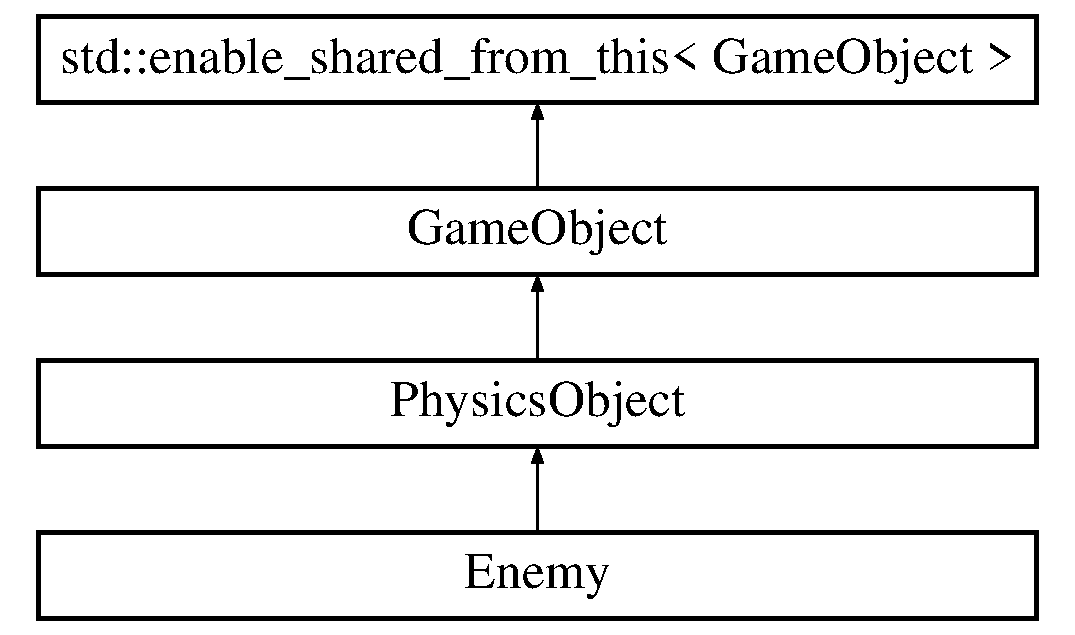
\includegraphics[height=4.000000cm]{dd/d7a/class_enemy}
\end{center}
\end{figure}
\subsection*{Public Member Functions}
\begin{DoxyCompactItemize}
\item 
\hyperlink{class_enemy_a0e382a7495bdbb9b802d1ed3931b4fc1}{Enemy} (const \hyperlink{class_physics_object}{Physics\+Object} \&physics\+Object, const double \&shoot\+Delay, const std\+::shared\+\_\+ptr$<$ \hyperlink{class_movable_interface}{Movable\+Interface} $>$ \&move\+Comp, const std\+::shared\+\_\+ptr$<$ \hyperlink{class_shoot_interface}{Shoot\+Interface} $>$ \&shoot\+Comp)
\begin{DoxyCompactList}\small\item\em Constructs the main enemy object used within the game. \end{DoxyCompactList}\item 
virtual void \hyperlink{class_enemy_a64ee0cc6fb8a3424d486537efb8205d8}{Start} () override
\begin{DoxyCompactList}\small\item\em Used to initialise the \hyperlink{class_enemy}{Enemy}. \end{DoxyCompactList}\item 
\mbox{\Hypertarget{class_enemy_a614ad271f07ecf63cb3e665155b7e258}\label{class_enemy_a614ad271f07ecf63cb3e665155b7e258}} 
virtual void \hyperlink{class_enemy_a614ad271f07ecf63cb3e665155b7e258}{Update} () override
\begin{DoxyCompactList}\small\item\em Runs once a frame and updates the various methods and members of the enemy. \end{DoxyCompactList}\item 
virtual void \hyperlink{class_enemy_ac59660a58fac8d0ffdcb97c0717fa089}{collision\+Action} (const Game\+Object\+Type \&object\+Type) override
\begin{DoxyCompactList}\small\item\em Checks if the enemy has collided with a player or player projectile and responds accordingly. \end{DoxyCompactList}\item 
void \hyperlink{class_enemy_a7fc3561fe6b79712b51bd06fa8ce24d0}{Assign\+Enemy\+Controller} (const std\+::shared\+\_\+ptr$<$ \hyperlink{class_game_object}{Game\+Object} $>$ \&enemy\+Controller)
\begin{DoxyCompactList}\small\item\em Assigns an enemy controller to the specific enemy, used to communicate with the enemy controller so that it knows whenever an enemy is destroyed. \end{DoxyCompactList}\item 
\mbox{\Hypertarget{class_enemy_aafb628c66008e33afdd750e2f492bd98}\label{class_enemy_aafb628c66008e33afdd750e2f492bd98}} 
virtual \hyperlink{class_enemy_aafb628c66008e33afdd750e2f492bd98}{$\sim$\+Enemy} ()=default
\begin{DoxyCompactList}\small\item\em Default Destructor. \end{DoxyCompactList}\end{DoxyCompactItemize}
\subsection*{Private Member Functions}
\begin{DoxyCompactItemize}
\item 
\mbox{\Hypertarget{class_enemy_ab526cfaf13910e15ca1e5e84ef230dd1}\label{class_enemy_ab526cfaf13910e15ca1e5e84ef230dd1}} 
void \hyperlink{class_enemy_ab526cfaf13910e15ca1e5e84ef230dd1}{Shoot} ()
\begin{DoxyCompactList}\small\item\em Determines if the shoot\+Delay is finished, if it is an \hyperlink{class_enemy_projectile}{Enemy\+Projectile} is created using the shoot\+Comp. \end{DoxyCompactList}\item 
\mbox{\Hypertarget{class_enemy_a06fafdc67bd76334adb9d47f73f15aff}\label{class_enemy_a06fafdc67bd76334adb9d47f73f15aff}} 
void \hyperlink{class_enemy_a06fafdc67bd76334adb9d47f73f15aff}{Check\+Outside\+Screen} ()
\begin{DoxyCompactList}\small\item\em Checks if the enemy is out of screen bounds. \end{DoxyCompactList}\item 
\hyperlink{class_vector2_d}{Vector2D} \hyperlink{class_enemy_aa40cb40a3a2d83e82e02ee5cfbb9ee96}{Generate\+Random\+Move\+Direction} ()
\begin{DoxyCompactList}\small\item\em Generates the random direction for the object to move in. \end{DoxyCompactList}\item 
\mbox{\Hypertarget{class_enemy_a9c4e7e1c9f79650d1f0dd3c72ae9c82d}\label{class_enemy_a9c4e7e1c9f79650d1f0dd3c72ae9c82d}} 
void \hyperlink{class_enemy_a9c4e7e1c9f79650d1f0dd3c72ae9c82d}{Player\+Projectile\+Collision} ()
\begin{DoxyCompactList}\small\item\em The Response of an Enemy\+Obejct to colliding with the player or the player bullet. \end{DoxyCompactList}\end{DoxyCompactItemize}
\subsection*{Private Attributes}
\begin{DoxyCompactItemize}
\item 
\hyperlink{class_delay_component}{Delay\+Component} \hyperlink{class_enemy_a3c5bc99471cfa718af8e11b3b735d15c}{\+\_\+shoot\+Delay}
\item 
std\+::shared\+\_\+ptr$<$ \hyperlink{class_shoot_interface}{Shoot\+Interface} $>$ \hyperlink{class_enemy_aab1e06a64c7fc2d07d40522a7a7cf8be}{\+\_\+enemy\+Shoot}
\item 
\hyperlink{class_boundary}{Boundary} \hyperlink{class_enemy_afb32f85ca2f3dce003e62a91572bdb70}{\+\_\+screen\+Bounds}
\item 
\hyperlink{class_size_reduction}{Size\+Reduction} \hyperlink{class_enemy_af8b4d39339f59407b7fd9cd1d6246860}{\+\_\+size\+Reduction}
\item 
std\+::shared\+\_\+ptr$<$ \hyperlink{class_movable_interface}{Movable\+Interface} $>$ \hyperlink{class_enemy_a1776f87f0a6993e9e3255c8a41c73809}{\+\_\+move\+Comp}
\item 
std\+::shared\+\_\+ptr$<$ \hyperlink{class_enemy_controller}{Enemy\+Controller} $>$ \hyperlink{class_enemy_acc360bdd3b46cea29891f534af2153c8}{\+\_\+enemy\+Controller}
\end{DoxyCompactItemize}
\subsection*{Additional Inherited Members}


\subsection{Detailed Description}
The basic \hyperlink{class_enemy}{Enemy} Object representation. 

Uses various interface composition objects to vary the behaviour of the \hyperlink{class_enemy}{Enemy} Object 

\subsection{Constructor \& Destructor Documentation}
\mbox{\Hypertarget{class_enemy_a0e382a7495bdbb9b802d1ed3931b4fc1}\label{class_enemy_a0e382a7495bdbb9b802d1ed3931b4fc1}} 
\index{Enemy@{Enemy}!Enemy@{Enemy}}
\index{Enemy@{Enemy}!Enemy@{Enemy}}
\subsubsection{\texorpdfstring{Enemy()}{Enemy()}}
{\footnotesize\ttfamily Enemy\+::\+Enemy (\begin{DoxyParamCaption}\item[{const \hyperlink{class_physics_object}{Physics\+Object} \&}]{physics\+Object,  }\item[{const double \&}]{shoot\+Delay,  }\item[{const std\+::shared\+\_\+ptr$<$ \hyperlink{class_movable_interface}{Movable\+Interface} $>$ \&}]{move\+Comp,  }\item[{const std\+::shared\+\_\+ptr$<$ \hyperlink{class_shoot_interface}{Shoot\+Interface} $>$ \&}]{shoot\+Comp }\end{DoxyParamCaption})}



Constructs the main enemy object used within the game. 


\begin{DoxyParams}{Parameters}
{\em physics\+Object} & The physics object information used to construct the enemy \\
\hline
{\em shoot\+Delay} & The \hyperlink{class_delay_component}{Delay\+Component} specified between enemy shots \\
\hline
{\em move\+Comp} & the \hyperlink{class_movable_interface}{Movable\+Interface} that the enemy uses \\
\hline
{\em shoot\+Comp} & The \hyperlink{class_shoot_interface}{Shoot\+Interface} used by the enemy\\
\hline
{\em physics\+Object} & \\
\hline
{\em shoot\+Delay} & \\
\hline
{\em move\+Comp} & \\
\hline
{\em shoot\+Comp} & \\
\hline
\end{DoxyParams}


\subsection{Member Function Documentation}
\mbox{\Hypertarget{class_enemy_a7fc3561fe6b79712b51bd06fa8ce24d0}\label{class_enemy_a7fc3561fe6b79712b51bd06fa8ce24d0}} 
\index{Enemy@{Enemy}!Assign\+Enemy\+Controller@{Assign\+Enemy\+Controller}}
\index{Assign\+Enemy\+Controller@{Assign\+Enemy\+Controller}!Enemy@{Enemy}}
\subsubsection{\texorpdfstring{Assign\+Enemy\+Controller()}{AssignEnemyController()}}
{\footnotesize\ttfamily void Enemy\+::\+Assign\+Enemy\+Controller (\begin{DoxyParamCaption}\item[{const std\+::shared\+\_\+ptr$<$ \hyperlink{class_game_object}{Game\+Object} $>$ \&}]{enemy\+Controller }\end{DoxyParamCaption})}



Assigns an enemy controller to the specific enemy, used to communicate with the enemy controller so that it knows whenever an enemy is destroyed. 


\begin{DoxyParams}{Parameters}
{\em enemy\+Controller} & shared pointer to the \hyperlink{class_enemy_controller}{Enemy\+Controller} that created the enemy \\
\hline
\end{DoxyParams}
\mbox{\Hypertarget{class_enemy_ac59660a58fac8d0ffdcb97c0717fa089}\label{class_enemy_ac59660a58fac8d0ffdcb97c0717fa089}} 
\index{Enemy@{Enemy}!collision\+Action@{collision\+Action}}
\index{collision\+Action@{collision\+Action}!Enemy@{Enemy}}
\subsubsection{\texorpdfstring{collision\+Action()}{collisionAction()}}
{\footnotesize\ttfamily void Enemy\+::collision\+Action (\begin{DoxyParamCaption}\item[{const Game\+Object\+Type \&}]{object\+Type }\end{DoxyParamCaption})\hspace{0.3cm}{\ttfamily [override]}, {\ttfamily [virtual]}}



Checks if the enemy has collided with a player or player projectile and responds accordingly. 


\begin{DoxyParams}{Parameters}
{\em object\+Type} & The type of object that has collided with the enemy \\
\hline
\end{DoxyParams}


Reimplemented from \hyperlink{class_physics_object_a16163f4e5bf781b3814d024c9f44a276}{Physics\+Object}.

\mbox{\Hypertarget{class_enemy_aa40cb40a3a2d83e82e02ee5cfbb9ee96}\label{class_enemy_aa40cb40a3a2d83e82e02ee5cfbb9ee96}} 
\index{Enemy@{Enemy}!Generate\+Random\+Move\+Direction@{Generate\+Random\+Move\+Direction}}
\index{Generate\+Random\+Move\+Direction@{Generate\+Random\+Move\+Direction}!Enemy@{Enemy}}
\subsubsection{\texorpdfstring{Generate\+Random\+Move\+Direction()}{GenerateRandomMoveDirection()}}
{\footnotesize\ttfamily \hyperlink{class_vector2_d}{Vector2D} Enemy\+::\+Generate\+Random\+Move\+Direction (\begin{DoxyParamCaption}{ }\end{DoxyParamCaption})\hspace{0.3cm}{\ttfamily [private]}}



Generates the random direction for the object to move in. 

\begin{DoxyReturn}{Returns}
Returns the generated random direction 
\end{DoxyReturn}
\mbox{\Hypertarget{class_enemy_a64ee0cc6fb8a3424d486537efb8205d8}\label{class_enemy_a64ee0cc6fb8a3424d486537efb8205d8}} 
\index{Enemy@{Enemy}!Start@{Start}}
\index{Start@{Start}!Enemy@{Enemy}}
\subsubsection{\texorpdfstring{Start()}{Start()}}
{\footnotesize\ttfamily void Enemy\+::\+Start (\begin{DoxyParamCaption}{ }\end{DoxyParamCaption})\hspace{0.3cm}{\ttfamily [override]}, {\ttfamily [virtual]}}



Used to initialise the \hyperlink{class_enemy}{Enemy}. 

ensures that the enemy is scaled correctly before it is displayed, and generates a random direction for its movement 

Reimplemented from \hyperlink{class_game_object_aeeb2162f2779e5591a372a1568bc5c68}{Game\+Object}.



\subsection{Member Data Documentation}
\mbox{\Hypertarget{class_enemy_acc360bdd3b46cea29891f534af2153c8}\label{class_enemy_acc360bdd3b46cea29891f534af2153c8}} 
\index{Enemy@{Enemy}!\+\_\+enemy\+Controller@{\+\_\+enemy\+Controller}}
\index{\+\_\+enemy\+Controller@{\+\_\+enemy\+Controller}!Enemy@{Enemy}}
\subsubsection{\texorpdfstring{\+\_\+enemy\+Controller}{\_enemyController}}
{\footnotesize\ttfamily std\+::shared\+\_\+ptr$<$\hyperlink{class_enemy_controller}{Enemy\+Controller}$>$ Enemy\+::\+\_\+enemy\+Controller\hspace{0.3cm}{\ttfamily [private]}}

\hyperlink{class_enemy_controller}{Enemy\+Controller} used to create the enemy object, is notified when the \hyperlink{class_enemy}{Enemy} object is destroyed \mbox{\Hypertarget{class_enemy_aab1e06a64c7fc2d07d40522a7a7cf8be}\label{class_enemy_aab1e06a64c7fc2d07d40522a7a7cf8be}} 
\index{Enemy@{Enemy}!\+\_\+enemy\+Shoot@{\+\_\+enemy\+Shoot}}
\index{\+\_\+enemy\+Shoot@{\+\_\+enemy\+Shoot}!Enemy@{Enemy}}
\subsubsection{\texorpdfstring{\+\_\+enemy\+Shoot}{\_enemyShoot}}
{\footnotesize\ttfamily std\+::shared\+\_\+ptr$<$\hyperlink{class_shoot_interface}{Shoot\+Interface}$>$ Enemy\+::\+\_\+enemy\+Shoot\hspace{0.3cm}{\ttfamily [private]}}

\hyperlink{class_shoot_interface}{Shoot\+Interface} used to specify the specific type of shooting \mbox{\Hypertarget{class_enemy_a1776f87f0a6993e9e3255c8a41c73809}\label{class_enemy_a1776f87f0a6993e9e3255c8a41c73809}} 
\index{Enemy@{Enemy}!\+\_\+move\+Comp@{\+\_\+move\+Comp}}
\index{\+\_\+move\+Comp@{\+\_\+move\+Comp}!Enemy@{Enemy}}
\subsubsection{\texorpdfstring{\+\_\+move\+Comp}{\_moveComp}}
{\footnotesize\ttfamily std\+::shared\+\_\+ptr$<$\hyperlink{class_movable_interface}{Movable\+Interface}$>$ Enemy\+::\+\_\+move\+Comp\hspace{0.3cm}{\ttfamily [private]}}

Moveable\+Interface used to move the enemy in a specific way \mbox{\Hypertarget{class_enemy_afb32f85ca2f3dce003e62a91572bdb70}\label{class_enemy_afb32f85ca2f3dce003e62a91572bdb70}} 
\index{Enemy@{Enemy}!\+\_\+screen\+Bounds@{\+\_\+screen\+Bounds}}
\index{\+\_\+screen\+Bounds@{\+\_\+screen\+Bounds}!Enemy@{Enemy}}
\subsubsection{\texorpdfstring{\+\_\+screen\+Bounds}{\_screenBounds}}
{\footnotesize\ttfamily \hyperlink{class_boundary}{Boundary} Enemy\+::\+\_\+screen\+Bounds\hspace{0.3cm}{\ttfamily [private]}}

Default boundary used to test if the enemy is outside of the screen \mbox{\Hypertarget{class_enemy_a3c5bc99471cfa718af8e11b3b735d15c}\label{class_enemy_a3c5bc99471cfa718af8e11b3b735d15c}} 
\index{Enemy@{Enemy}!\+\_\+shoot\+Delay@{\+\_\+shoot\+Delay}}
\index{\+\_\+shoot\+Delay@{\+\_\+shoot\+Delay}!Enemy@{Enemy}}
\subsubsection{\texorpdfstring{\+\_\+shoot\+Delay}{\_shootDelay}}
{\footnotesize\ttfamily \hyperlink{class_delay_component}{Delay\+Component} Enemy\+::\+\_\+shoot\+Delay\hspace{0.3cm}{\ttfamily [private]}}

delay used between each shot per object \mbox{\Hypertarget{class_enemy_af8b4d39339f59407b7fd9cd1d6246860}\label{class_enemy_af8b4d39339f59407b7fd9cd1d6246860}} 
\index{Enemy@{Enemy}!\+\_\+size\+Reduction@{\+\_\+size\+Reduction}}
\index{\+\_\+size\+Reduction@{\+\_\+size\+Reduction}!Enemy@{Enemy}}
\subsubsection{\texorpdfstring{\+\_\+size\+Reduction}{\_sizeReduction}}
{\footnotesize\ttfamily \hyperlink{class_size_reduction}{Size\+Reduction} Enemy\+::\+\_\+size\+Reduction\hspace{0.3cm}{\ttfamily [private]}}

\hyperlink{class_size_reduction}{Size\+Reduction} component used to scale the enemy as it moves towards or away from the centre of the screen 

The documentation for this class was generated from the following files\+:\begin{DoxyCompactItemize}
\item 
D\+:/\+Users/\+Tim-\/\+P\+C/\+Documents/\+Software\+\_\+\+I\+I/\+Project/\+Project\+Files/game-\/source-\/code/\+Front\+End\+Systems/Enemy.\+h\item 
D\+:/\+Users/\+Tim-\/\+P\+C/\+Documents/\+Software\+\_\+\+I\+I/\+Project/\+Project\+Files/game-\/source-\/code/\+Front\+End\+Systems/Enemy.\+cpp\end{DoxyCompactItemize}

\hypertarget{class_enemy_controller}{}\section{Enemy\+Controller Class Reference}
\label{class_enemy_controller}\index{Enemy\+Controller@{Enemy\+Controller}}


\hyperlink{class_enemy}{Enemy} controller is responsible for spawning and monitoring new enemy objects.  




{\ttfamily \#include $<$Enemy\+Controller.\+h$>$}

Inheritance diagram for Enemy\+Controller\+:\begin{figure}[H]
\begin{center}
\leavevmode
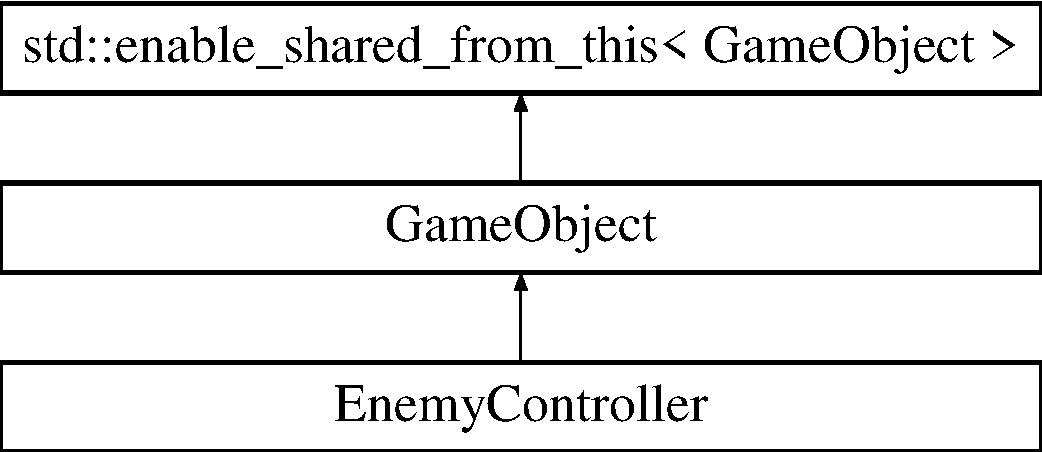
\includegraphics[height=3.000000cm]{dc/d01/class_enemy_controller}
\end{center}
\end{figure}
\subsection*{Public Member Functions}
\begin{DoxyCompactItemize}
\item 
\hyperlink{class_enemy_controller_a07159de6348f511017c5415371459d50}{Enemy\+Controller} (const \hyperlink{class_game_object}{Game\+Object} \&game\+Object, unsigned int max\+\_\+enemies, double enemy\+Spawn\+Delay)
\begin{DoxyCompactList}\small\item\em Constructs an \hyperlink{class_enemy_controller}{Enemy\+Controller} Object. \end{DoxyCompactList}\item 
\mbox{\Hypertarget{class_enemy_controller_af36ec67442d30c7519581b83ad6c00db}\label{class_enemy_controller_af36ec67442d30c7519581b83ad6c00db}} 
virtual void \hyperlink{class_enemy_controller_af36ec67442d30c7519581b83ad6c00db}{Update} () override
\begin{DoxyCompactList}\small\item\em Creates enemies based on the spawn delay. \end{DoxyCompactList}\item 
\mbox{\Hypertarget{class_enemy_controller_a011030dd51b78317ecb16356bf6591dc}\label{class_enemy_controller_a011030dd51b78317ecb16356bf6591dc}} 
void \hyperlink{class_enemy_controller_a011030dd51b78317ecb16356bf6591dc}{Enemy\+Killed} ()
\begin{DoxyCompactList}\small\item\em Called by the Enemy\+Object to inform the \hyperlink{class_enemy_controller}{Enemy\+Controller} that it has been destroyed by the \hyperlink{class_player}{Player} object. \end{DoxyCompactList}\item 
void \hyperlink{class_enemy_controller_a182dba707716f8079bb6e67e8c5ed4ad}{Enemy\+Outof\+Bounds} ()
\begin{DoxyCompactList}\small\item\em Called by the Enemy\+Object to inform the \hyperlink{class_enemy_controller}{Enemy\+Controller} that it has been destroyed by the moving out of bounds. \end{DoxyCompactList}\end{DoxyCompactItemize}
\subsection*{Private Member Functions}
\begin{DoxyCompactItemize}
\item 
\mbox{\Hypertarget{class_enemy_controller_a84eabc12a38617b5ff05c6e896e97531}\label{class_enemy_controller_a84eabc12a38617b5ff05c6e896e97531}} 
void \hyperlink{class_enemy_controller_a84eabc12a38617b5ff05c6e896e97531}{Spawn\+Enemy\+Count\+Down} ()
\begin{DoxyCompactList}\small\item\em Checks if an \hyperlink{class_enemy}{Enemy} can be spawned due to the spawn delay, calls Spawn\+Enemy if it can be. \end{DoxyCompactList}\item 
\mbox{\Hypertarget{class_enemy_controller_ab5298e79a0bf598ed8684efb8a6a3927}\label{class_enemy_controller_ab5298e79a0bf598ed8684efb8a6a3927}} 
void \hyperlink{class_enemy_controller_ab5298e79a0bf598ed8684efb8a6a3927}{Spawn\+Enemy} ()
\begin{DoxyCompactList}\small\item\em Creates an enemy and adds it to the same \hyperlink{class_scene}{Scene} as the \hyperlink{class_enemy_controller}{Enemy\+Controller}. \end{DoxyCompactList}\end{DoxyCompactItemize}
\subsection*{Private Attributes}
\begin{DoxyCompactItemize}
\item 
unsigned int \hyperlink{class_enemy_controller_a2b2fdb5b40b75f719838da0386861da5}{number\+Of\+Enemies\+Killed}
\item 
const unsigned int \hyperlink{class_enemy_controller_aca04264b909526dadc67a41f8c826aee}{M\+A\+X\+\_\+\+N\+U\+M\+B\+E\+R\+\_\+\+O\+F\+\_\+\+E\+N\+E\+M\+I\+ES}
\item 
\hyperlink{class_delay_component}{Delay\+Component} \hyperlink{class_enemy_controller_af6136b2e8750227e8adf729c9de5232b}{\+\_\+enemy\+Spawn\+Delay}
\item 
unsigned int \hyperlink{class_enemy_controller_a673e9320e737999189b943216f6d379b}{enemy\+Count}
\end{DoxyCompactItemize}
\subsection*{Additional Inherited Members}


\subsection{Detailed Description}
\hyperlink{class_enemy}{Enemy} controller is responsible for spawning and monitoring new enemy objects. 

The number of enemies spawned and destroyed is moitored. When an enemy goes out of bounds it is destroyed and created a new. The enemy objects have access to the \hyperlink{class_enemy_controller}{Enemy\+Controller} to communicate with it when they are destroyed by the player and when they leave the bounds of the screen. If all the enemies have been destroyed the \hyperlink{class_enemy_controller}{Enemy\+Controller} changes scenes to the Win\+Screen 

\subsection{Constructor \& Destructor Documentation}
\mbox{\Hypertarget{class_enemy_controller_a07159de6348f511017c5415371459d50}\label{class_enemy_controller_a07159de6348f511017c5415371459d50}} 
\index{Enemy\+Controller@{Enemy\+Controller}!Enemy\+Controller@{Enemy\+Controller}}
\index{Enemy\+Controller@{Enemy\+Controller}!Enemy\+Controller@{Enemy\+Controller}}
\subsubsection{\texorpdfstring{Enemy\+Controller()}{EnemyController()}}
{\footnotesize\ttfamily Enemy\+Controller\+::\+Enemy\+Controller (\begin{DoxyParamCaption}\item[{const \hyperlink{class_game_object}{Game\+Object} \&}]{game\+Object,  }\item[{unsigned int}]{max\+\_\+enemies,  }\item[{double}]{enemy\+Spawn\+Delay }\end{DoxyParamCaption})}



Constructs an \hyperlink{class_enemy_controller}{Enemy\+Controller} Object. 


\begin{DoxyParams}{Parameters}
{\em max\+\_\+enemies} & The maximum number of enemies that the \hyperlink{class_enemy_controller}{Enemy\+Controller} will create \\
\hline
{\em enemy\+Spawn\+Delay} & The time delay between spawning an enemy object \\
\hline
\end{DoxyParams}


\subsection{Member Function Documentation}
\mbox{\Hypertarget{class_enemy_controller_a182dba707716f8079bb6e67e8c5ed4ad}\label{class_enemy_controller_a182dba707716f8079bb6e67e8c5ed4ad}} 
\index{Enemy\+Controller@{Enemy\+Controller}!Enemy\+Outof\+Bounds@{Enemy\+Outof\+Bounds}}
\index{Enemy\+Outof\+Bounds@{Enemy\+Outof\+Bounds}!Enemy\+Controller@{Enemy\+Controller}}
\subsubsection{\texorpdfstring{Enemy\+Outof\+Bounds()}{EnemyOutofBounds()}}
{\footnotesize\ttfamily void Enemy\+Controller\+::\+Enemy\+Outof\+Bounds (\begin{DoxyParamCaption}{ }\end{DoxyParamCaption})}



Called by the Enemy\+Object to inform the \hyperlink{class_enemy_controller}{Enemy\+Controller} that it has been destroyed by the moving out of bounds. 

spawns a new enemy without checking the delay as the enemy has already been spawned 

\subsection{Member Data Documentation}
\mbox{\Hypertarget{class_enemy_controller_af6136b2e8750227e8adf729c9de5232b}\label{class_enemy_controller_af6136b2e8750227e8adf729c9de5232b}} 
\index{Enemy\+Controller@{Enemy\+Controller}!\+\_\+enemy\+Spawn\+Delay@{\+\_\+enemy\+Spawn\+Delay}}
\index{\+\_\+enemy\+Spawn\+Delay@{\+\_\+enemy\+Spawn\+Delay}!Enemy\+Controller@{Enemy\+Controller}}
\subsubsection{\texorpdfstring{\+\_\+enemy\+Spawn\+Delay}{\_enemySpawnDelay}}
{\footnotesize\ttfamily \hyperlink{class_delay_component}{Delay\+Component} Enemy\+Controller\+::\+\_\+enemy\+Spawn\+Delay\hspace{0.3cm}{\ttfamily [private]}}

The delay component used to track the delay between enemy spawns \mbox{\Hypertarget{class_enemy_controller_a673e9320e737999189b943216f6d379b}\label{class_enemy_controller_a673e9320e737999189b943216f6d379b}} 
\index{Enemy\+Controller@{Enemy\+Controller}!enemy\+Count@{enemy\+Count}}
\index{enemy\+Count@{enemy\+Count}!Enemy\+Controller@{Enemy\+Controller}}
\subsubsection{\texorpdfstring{enemy\+Count}{enemyCount}}
{\footnotesize\ttfamily unsigned int Enemy\+Controller\+::enemy\+Count\hspace{0.3cm}{\ttfamily [private]}}

The current number of enemies that have been spawned \mbox{\Hypertarget{class_enemy_controller_aca04264b909526dadc67a41f8c826aee}\label{class_enemy_controller_aca04264b909526dadc67a41f8c826aee}} 
\index{Enemy\+Controller@{Enemy\+Controller}!M\+A\+X\+\_\+\+N\+U\+M\+B\+E\+R\+\_\+\+O\+F\+\_\+\+E\+N\+E\+M\+I\+ES@{M\+A\+X\+\_\+\+N\+U\+M\+B\+E\+R\+\_\+\+O\+F\+\_\+\+E\+N\+E\+M\+I\+ES}}
\index{M\+A\+X\+\_\+\+N\+U\+M\+B\+E\+R\+\_\+\+O\+F\+\_\+\+E\+N\+E\+M\+I\+ES@{M\+A\+X\+\_\+\+N\+U\+M\+B\+E\+R\+\_\+\+O\+F\+\_\+\+E\+N\+E\+M\+I\+ES}!Enemy\+Controller@{Enemy\+Controller}}
\subsubsection{\texorpdfstring{M\+A\+X\+\_\+\+N\+U\+M\+B\+E\+R\+\_\+\+O\+F\+\_\+\+E\+N\+E\+M\+I\+ES}{MAX\_NUMBER\_OF\_ENEMIES}}
{\footnotesize\ttfamily const unsigned int Enemy\+Controller\+::\+M\+A\+X\+\_\+\+N\+U\+M\+B\+E\+R\+\_\+\+O\+F\+\_\+\+E\+N\+E\+M\+I\+ES\hspace{0.3cm}{\ttfamily [private]}}

The maximum number of enemies that the \hyperlink{class_enemy_controller}{Enemy\+Controller} can create \mbox{\Hypertarget{class_enemy_controller_a2b2fdb5b40b75f719838da0386861da5}\label{class_enemy_controller_a2b2fdb5b40b75f719838da0386861da5}} 
\index{Enemy\+Controller@{Enemy\+Controller}!number\+Of\+Enemies\+Killed@{number\+Of\+Enemies\+Killed}}
\index{number\+Of\+Enemies\+Killed@{number\+Of\+Enemies\+Killed}!Enemy\+Controller@{Enemy\+Controller}}
\subsubsection{\texorpdfstring{number\+Of\+Enemies\+Killed}{numberOfEnemiesKilled}}
{\footnotesize\ttfamily unsigned int Enemy\+Controller\+::number\+Of\+Enemies\+Killed\hspace{0.3cm}{\ttfamily [private]}}

Tracks the number of enemies that the player has destroyed 

The documentation for this class was generated from the following files\+:\begin{DoxyCompactItemize}
\item 
C\+:/\+Users/\+Tim/\+Documents/\+Software\+Dev/\+Software\+Project/\+Project\+Files/game-\/source-\/code/\+Front\+End\+Systems/Enemy\+Controller.\+h\item 
C\+:/\+Users/\+Tim/\+Documents/\+Software\+Dev/\+Software\+Project/\+Project\+Files/game-\/source-\/code/\+Front\+End\+Systems/Enemy\+Controller.\+cpp\end{DoxyCompactItemize}

\hypertarget{class_event_manager}{}\section{Event\+Manager Class Reference}
\label{class_event_manager}\index{Event\+Manager@{Event\+Manager}}


can be converted into a singleton  




{\ttfamily \#include $<$Event\+Manager.\+h$>$}

\subsection*{Public Member Functions}
\begin{DoxyCompactItemize}
\item 
\mbox{\Hypertarget{class_event_manager_a89099b22114f158b5c530edfea52371d}\label{class_event_manager_a89099b22114f158b5c530edfea52371d}} 
\hyperlink{class_event_manager_a89099b22114f158b5c530edfea52371d}{Event\+Manager} ()
\begin{DoxyCompactList}\small\item\em redundant constructors should be removed, only a default is necessary with the event loop function \end{DoxyCompactList}\item 
\mbox{\Hypertarget{class_event_manager_a8951d1cf3aabe678cd37c64317497519}\label{class_event_manager_a8951d1cf3aabe678cd37c64317497519}} 
{\bfseries Event\+Manager} (Render\+Window $\ast$event\+Window)
\item 
\mbox{\Hypertarget{class_event_manager_a3e90c3658f1fc88b45ba1b8fda4f2c10}\label{class_event_manager_a3e90c3658f1fc88b45ba1b8fda4f2c10}} 
void {\bfseries Event\+Loop} (Render\+Window \&event\+Window)
\end{DoxyCompactItemize}
\subsection*{Private Member Functions}
\begin{DoxyCompactItemize}
\item 
\mbox{\Hypertarget{class_event_manager_a279b1d4e14cd98c1b3789a5276be2b3a}\label{class_event_manager_a279b1d4e14cd98c1b3789a5276be2b3a}} 
void {\bfseries Key\+Input} (const Event \&event, bool state)
\end{DoxyCompactItemize}
\subsection*{Private Attributes}
\begin{DoxyCompactItemize}
\item 
\mbox{\Hypertarget{class_event_manager_a1909a88890831dfd326b4a9032c48ac2}\label{class_event_manager_a1909a88890831dfd326b4a9032c48ac2}} 
std\+::shared\+\_\+ptr$<$ Render\+Window $>$ \hyperlink{class_event_manager_a1909a88890831dfd326b4a9032c48ac2}{\+\_\+event\+Window}
\begin{DoxyCompactList}\small\item\em redundant shared pointer \end{DoxyCompactList}\end{DoxyCompactItemize}


\subsection{Detailed Description}
can be converted into a singleton 

The documentation for this class was generated from the following files\+:\begin{DoxyCompactItemize}
\item 
D\+:/\+Users/\+Tim-\/\+P\+C/\+Documents/\+Software\+\_\+\+I\+I/\+Project/\+Project\+Files/game-\/source-\/code/\+Back\+End\+Systems/Event\+Manager.\+h\item 
D\+:/\+Users/\+Tim-\/\+P\+C/\+Documents/\+Software\+\_\+\+I\+I/\+Project/\+Project\+Files/game-\/source-\/code/\+Back\+End\+Systems/Event\+Manager.\+cpp\end{DoxyCompactItemize}

\hypertarget{class_failed_to_load_texture}{}\section{Failed\+To\+Load\+Texture Class Reference}
\label{class_failed_to_load_texture}\index{Failed\+To\+Load\+Texture@{Failed\+To\+Load\+Texture}}


The documentation for this class was generated from the following file\+:\begin{DoxyCompactItemize}
\item 
D\+:/\+Users/\+Tim-\/\+P\+C/\+Documents/\+Software\+\_\+\+I\+I/\+Project/\+Project\+Files/game-\/source-\/code/\+Back\+End\+Systems/Display\+Manger.\+cpp\end{DoxyCompactItemize}

\hypertarget{class_game_manager}{}\section{Game\+Manager Class Reference}
\label{class_game_manager}\index{Game\+Manager@{Game\+Manager}}


\hyperlink{class_game_manager}{Game\+Manager} is responsible for intialising and maintaining the game state, and updating the game loop through the composition of different \hyperlink{class_scene}{Scene} objects that exist within the game, it communicates with the \hyperlink{class_event_manager}{Event\+Manager}, \hyperlink{class_display_manager}{Display\+Manager} and \hyperlink{class_collision_detection}{Collision\+Detection} classes regarding the state of the game.  




{\ttfamily \#include $<$Game\+Manager.\+h$>$}

\subsection*{Public Member Functions}
\begin{DoxyCompactItemize}
\item 
\hyperlink{class_game_manager_a05f6a37de95fcea1313fe4476b95941d}{Game\+Manager} (std\+::shared\+\_\+ptr$<$ \hyperlink{class_repositiory_interface}{Repositiory\+Interface} $>$ repository)
\begin{DoxyCompactList}\small\item\em Constructs the \hyperlink{class_game_manager}{Game\+Manager} object neccesary for the Game loop. \end{DoxyCompactList}\item 
\mbox{\Hypertarget{class_game_manager_a5baa570812ae717f809fe0dc48bde22e}\label{class_game_manager_a5baa570812ae717f809fe0dc48bde22e}} 
void \hyperlink{class_game_manager_a5baa570812ae717f809fe0dc48bde22e}{Game\+Loop} ()
\begin{DoxyCompactList}\small\item\em Runs the main game loop of the game, and updates the various Game\+Objects Stored inside of the active\+Scene. \end{DoxyCompactList}\item 
void \hyperlink{class_game_manager_a09b8801bcfdd8d5cbc52e27895b84e3b}{Load\+Scene} (unsigned int index)
\begin{DoxyCompactList}\small\item\em Changes the active \hyperlink{class_scene}{Scene} to the \hyperlink{class_scene}{Scene} at the desired Scene\+Index. \end{DoxyCompactList}\end{DoxyCompactItemize}
\subsection*{Static Public Member Functions}
\begin{DoxyCompactItemize}
\item 
static void \hyperlink{class_game_manager_acbd9fb84f9e18c8cb585738d5c89a2b9}{Exit} ()
\begin{DoxyCompactList}\small\item\em Closes the game window. \end{DoxyCompactList}\item 
static int \hyperlink{class_game_manager_aa4835b5fc96bfdbf6170a8673baf5552}{get\+Scene\+Index} ()
\begin{DoxyCompactList}\small\item\em Returns the current scene index. \end{DoxyCompactList}\item 
static const bool \hyperlink{class_game_manager_a4eb94c6171bf3292eb57b291e2174289}{game\+Closed} ()
\begin{DoxyCompactList}\small\item\em Identifies whether the game has been closed. \end{DoxyCompactList}\end{DoxyCompactItemize}
\subsection*{Static Public Attributes}
\begin{DoxyCompactItemize}
\item 
static std\+::shared\+\_\+ptr$<$ \hyperlink{class_scene}{Scene} $>$ \hyperlink{class_game_manager_a969dd909c6b70310843d34e2490736b4}{active\+Scene} = N\+U\+LL
\end{DoxyCompactItemize}
\subsection*{Private Member Functions}
\begin{DoxyCompactItemize}
\item 
void \hyperlink{class_game_manager_a0a4c03ef0451371a98204c18c1faf9fd}{initialise\+Window} (sf\+::\+Render\+Window \&\+\_\+game\+Window)
\begin{DoxyCompactList}\small\item\em Initialises the sfml Render\+Window to the properties defined by the default window settings. \end{DoxyCompactList}\end{DoxyCompactItemize}
\subsection*{Private Attributes}
\begin{DoxyCompactItemize}
\item 
std\+::shared\+\_\+ptr$<$ \hyperlink{class_repositiory_interface}{Repositiory\+Interface} $>$ \hyperlink{class_game_manager_adf8ffad3969c2bee2332eb3ea58a3c9c}{\+\_\+repository}
\item 
sf\+::\+Render\+Window \hyperlink{class_game_manager_a0c91609e7557e4e97a0e4be541254a38}{\+\_\+window}
\item 
std\+::unique\+\_\+ptr$<$ \hyperlink{class_game_time}{Game\+Time} $>$ \hyperlink{class_game_manager_ae08fe7df616e789e4858645b56d9b73b}{\+\_\+game\+Time}
\item 
\hyperlink{struct_window_settings}{Window\+Settings} \hyperlink{class_game_manager_a06843f28cb1609e41da7eee19be9aa87}{\+\_\+default\+Setup}
\item 
std\+::vector$<$ std\+::shared\+\_\+ptr$<$ \hyperlink{class_scene}{Scene} $>$ $>$ \hyperlink{class_game_manager_a6be6c6b38c1b95d7fd84819eba50e618}{\+\_\+game\+\_\+scenes}
\end{DoxyCompactItemize}
\subsection*{Static Private Attributes}
\begin{DoxyCompactItemize}
\item 
static int \hyperlink{class_game_manager_aedb575ca538853f3d7053b33bef238e0}{\+\_\+scene\+\_\+index} = 0
\item 
static bool \hyperlink{class_game_manager_a07c75a9507a0d82f88a0b62d808fcf3c}{close\+Window} = false
\end{DoxyCompactItemize}


\subsection{Detailed Description}
\hyperlink{class_game_manager}{Game\+Manager} is responsible for intialising and maintaining the game state, and updating the game loop through the composition of different \hyperlink{class_scene}{Scene} objects that exist within the game, it communicates with the \hyperlink{class_event_manager}{Event\+Manager}, \hyperlink{class_display_manager}{Display\+Manager} and \hyperlink{class_collision_detection}{Collision\+Detection} classes regarding the state of the game. 

\subsection{Constructor \& Destructor Documentation}
\mbox{\Hypertarget{class_game_manager_a05f6a37de95fcea1313fe4476b95941d}\label{class_game_manager_a05f6a37de95fcea1313fe4476b95941d}} 
\index{Game\+Manager@{Game\+Manager}!Game\+Manager@{Game\+Manager}}
\index{Game\+Manager@{Game\+Manager}!Game\+Manager@{Game\+Manager}}
\subsubsection{\texorpdfstring{Game\+Manager()}{GameManager()}}
{\footnotesize\ttfamily Game\+Manager\+::\+Game\+Manager (\begin{DoxyParamCaption}\item[{std\+::shared\+\_\+ptr$<$ \hyperlink{class_repositiory_interface}{Repositiory\+Interface} $>$}]{repository }\end{DoxyParamCaption})}



Constructs the \hyperlink{class_game_manager}{Game\+Manager} object neccesary for the Game loop. 


\begin{DoxyParams}{Parameters}
{\em repository} & The instance of the \hyperlink{class_repository}{Repository} used to generate the Scenes for the game \\
\hline
\end{DoxyParams}


\subsection{Member Function Documentation}
\mbox{\Hypertarget{class_game_manager_acbd9fb84f9e18c8cb585738d5c89a2b9}\label{class_game_manager_acbd9fb84f9e18c8cb585738d5c89a2b9}} 
\index{Game\+Manager@{Game\+Manager}!Exit@{Exit}}
\index{Exit@{Exit}!Game\+Manager@{Game\+Manager}}
\subsubsection{\texorpdfstring{Exit()}{Exit()}}
{\footnotesize\ttfamily void Game\+Manager\+::\+Exit (\begin{DoxyParamCaption}{ }\end{DoxyParamCaption})\hspace{0.3cm}{\ttfamily [static]}}



Closes the game window. 

Exit function needs to be moved into \hyperlink{class_scene}{Scene} or a seperate \hyperlink{class_application}{Application} class. \mbox{\Hypertarget{class_game_manager_a4eb94c6171bf3292eb57b291e2174289}\label{class_game_manager_a4eb94c6171bf3292eb57b291e2174289}} 
\index{Game\+Manager@{Game\+Manager}!game\+Closed@{game\+Closed}}
\index{game\+Closed@{game\+Closed}!Game\+Manager@{Game\+Manager}}
\subsubsection{\texorpdfstring{game\+Closed()}{gameClosed()}}
{\footnotesize\ttfamily static const bool Game\+Manager\+::game\+Closed (\begin{DoxyParamCaption}{ }\end{DoxyParamCaption})\hspace{0.3cm}{\ttfamily [inline]}, {\ttfamily [static]}}



Identifies whether the game has been closed. 

\begin{DoxyReturn}{Returns}
Returns a constant bool whether the game is closed 
\end{DoxyReturn}
\mbox{\Hypertarget{class_game_manager_aa4835b5fc96bfdbf6170a8673baf5552}\label{class_game_manager_aa4835b5fc96bfdbf6170a8673baf5552}} 
\index{Game\+Manager@{Game\+Manager}!get\+Scene\+Index@{get\+Scene\+Index}}
\index{get\+Scene\+Index@{get\+Scene\+Index}!Game\+Manager@{Game\+Manager}}
\subsubsection{\texorpdfstring{get\+Scene\+Index()}{getSceneIndex()}}
{\footnotesize\ttfamily static int Game\+Manager\+::get\+Scene\+Index (\begin{DoxyParamCaption}{ }\end{DoxyParamCaption})\hspace{0.3cm}{\ttfamily [inline]}, {\ttfamily [static]}}



Returns the current scene index. 

\begin{DoxyReturn}{Returns}
The Current \hyperlink{class_scene}{Scene} Index 
\end{DoxyReturn}
\mbox{\Hypertarget{class_game_manager_a0a4c03ef0451371a98204c18c1faf9fd}\label{class_game_manager_a0a4c03ef0451371a98204c18c1faf9fd}} 
\index{Game\+Manager@{Game\+Manager}!initialise\+Window@{initialise\+Window}}
\index{initialise\+Window@{initialise\+Window}!Game\+Manager@{Game\+Manager}}
\subsubsection{\texorpdfstring{initialise\+Window()}{initialiseWindow()}}
{\footnotesize\ttfamily void Game\+Manager\+::initialise\+Window (\begin{DoxyParamCaption}\item[{sf\+::\+Render\+Window \&}]{\+\_\+game\+Window }\end{DoxyParamCaption})\hspace{0.3cm}{\ttfamily [private]}}



Initialises the sfml Render\+Window to the properties defined by the default window settings. 


\begin{DoxyParams}{Parameters}
{\em \+\_\+game\+Window} & \\
\hline
\end{DoxyParams}
\mbox{\Hypertarget{class_game_manager_a09b8801bcfdd8d5cbc52e27895b84e3b}\label{class_game_manager_a09b8801bcfdd8d5cbc52e27895b84e3b}} 
\index{Game\+Manager@{Game\+Manager}!Load\+Scene@{Load\+Scene}}
\index{Load\+Scene@{Load\+Scene}!Game\+Manager@{Game\+Manager}}
\subsubsection{\texorpdfstring{Load\+Scene()}{LoadScene()}}
{\footnotesize\ttfamily void Game\+Manager\+::\+Load\+Scene (\begin{DoxyParamCaption}\item[{unsigned int}]{index }\end{DoxyParamCaption})}



Changes the active \hyperlink{class_scene}{Scene} to the \hyperlink{class_scene}{Scene} at the desired Scene\+Index. 

Should be called from an application class but remains inside of game\+Manager.


\begin{DoxyParams}{Parameters}
{\em index} & The index for which the desired scene is located \\
\hline
\end{DoxyParams}


\subsection{Member Data Documentation}
\mbox{\Hypertarget{class_game_manager_a06843f28cb1609e41da7eee19be9aa87}\label{class_game_manager_a06843f28cb1609e41da7eee19be9aa87}} 
\index{Game\+Manager@{Game\+Manager}!\+\_\+default\+Setup@{\+\_\+default\+Setup}}
\index{\+\_\+default\+Setup@{\+\_\+default\+Setup}!Game\+Manager@{Game\+Manager}}
\subsubsection{\texorpdfstring{\+\_\+default\+Setup}{\_defaultSetup}}
{\footnotesize\ttfamily \hyperlink{struct_window_settings}{Window\+Settings} Game\+Manager\+::\+\_\+default\+Setup\hspace{0.3cm}{\ttfamily [private]}}

the default Setup information for the game \mbox{\Hypertarget{class_game_manager_a6be6c6b38c1b95d7fd84819eba50e618}\label{class_game_manager_a6be6c6b38c1b95d7fd84819eba50e618}} 
\index{Game\+Manager@{Game\+Manager}!\+\_\+game\+\_\+scenes@{\+\_\+game\+\_\+scenes}}
\index{\+\_\+game\+\_\+scenes@{\+\_\+game\+\_\+scenes}!Game\+Manager@{Game\+Manager}}
\subsubsection{\texorpdfstring{\+\_\+game\+\_\+scenes}{\_game\_scenes}}
{\footnotesize\ttfamily std\+::vector$<$std\+::shared\+\_\+ptr$<$\hyperlink{class_scene}{Scene}$>$ $>$ Game\+Manager\+::\+\_\+game\+\_\+scenes\hspace{0.3cm}{\ttfamily [private]}}

A vector of \hyperlink{class_scene}{Scene} Objects used to represent the different Scenes of the game \mbox{\Hypertarget{class_game_manager_ae08fe7df616e789e4858645b56d9b73b}\label{class_game_manager_ae08fe7df616e789e4858645b56d9b73b}} 
\index{Game\+Manager@{Game\+Manager}!\+\_\+game\+Time@{\+\_\+game\+Time}}
\index{\+\_\+game\+Time@{\+\_\+game\+Time}!Game\+Manager@{Game\+Manager}}
\subsubsection{\texorpdfstring{\+\_\+game\+Time}{\_gameTime}}
{\footnotesize\ttfamily std\+::unique\+\_\+ptr$<$\hyperlink{class_game_time}{Game\+Time}$>$ Game\+Manager\+::\+\_\+game\+Time\hspace{0.3cm}{\ttfamily [private]}}

A unique pointer to a \hyperlink{class_game_time}{Game\+Time} object, used to update the time between frames \mbox{\Hypertarget{class_game_manager_adf8ffad3969c2bee2332eb3ea58a3c9c}\label{class_game_manager_adf8ffad3969c2bee2332eb3ea58a3c9c}} 
\index{Game\+Manager@{Game\+Manager}!\+\_\+repository@{\+\_\+repository}}
\index{\+\_\+repository@{\+\_\+repository}!Game\+Manager@{Game\+Manager}}
\subsubsection{\texorpdfstring{\+\_\+repository}{\_repository}}
{\footnotesize\ttfamily std\+::shared\+\_\+ptr$<$\hyperlink{class_repositiory_interface}{Repositiory\+Interface}$>$ Game\+Manager\+::\+\_\+repository\hspace{0.3cm}{\ttfamily [private]}}

The Repository\+Interface used to generate the Scenes for the game \mbox{\Hypertarget{class_game_manager_aedb575ca538853f3d7053b33bef238e0}\label{class_game_manager_aedb575ca538853f3d7053b33bef238e0}} 
\index{Game\+Manager@{Game\+Manager}!\+\_\+scene\+\_\+index@{\+\_\+scene\+\_\+index}}
\index{\+\_\+scene\+\_\+index@{\+\_\+scene\+\_\+index}!Game\+Manager@{Game\+Manager}}
\subsubsection{\texorpdfstring{\+\_\+scene\+\_\+index}{\_scene\_index}}
{\footnotesize\ttfamily int Game\+Manager\+::\+\_\+scene\+\_\+index = 0\hspace{0.3cm}{\ttfamily [static]}, {\ttfamily [private]}}

The current \hyperlink{class_scene}{Scene} Index for the game \mbox{\Hypertarget{class_game_manager_a0c91609e7557e4e97a0e4be541254a38}\label{class_game_manager_a0c91609e7557e4e97a0e4be541254a38}} 
\index{Game\+Manager@{Game\+Manager}!\+\_\+window@{\+\_\+window}}
\index{\+\_\+window@{\+\_\+window}!Game\+Manager@{Game\+Manager}}
\subsubsection{\texorpdfstring{\+\_\+window}{\_window}}
{\footnotesize\ttfamily sf\+::\+Render\+Window Game\+Manager\+::\+\_\+window\hspace{0.3cm}{\ttfamily [private]}}

The sfml Render\+Window used for the game \mbox{\Hypertarget{class_game_manager_a969dd909c6b70310843d34e2490736b4}\label{class_game_manager_a969dd909c6b70310843d34e2490736b4}} 
\index{Game\+Manager@{Game\+Manager}!active\+Scene@{active\+Scene}}
\index{active\+Scene@{active\+Scene}!Game\+Manager@{Game\+Manager}}
\subsubsection{\texorpdfstring{active\+Scene}{activeScene}}
{\footnotesize\ttfamily std\+::shared\+\_\+ptr$<$ \hyperlink{class_scene}{Scene} $>$ Game\+Manager\+::active\+Scene = N\+U\+LL\hspace{0.3cm}{\ttfamily [static]}}

public static variable that represents the active \hyperlink{class_scene}{Scene} -\/ Bad design reveals too much information \mbox{\Hypertarget{class_game_manager_a07c75a9507a0d82f88a0b62d808fcf3c}\label{class_game_manager_a07c75a9507a0d82f88a0b62d808fcf3c}} 
\index{Game\+Manager@{Game\+Manager}!close\+Window@{close\+Window}}
\index{close\+Window@{close\+Window}!Game\+Manager@{Game\+Manager}}
\subsubsection{\texorpdfstring{close\+Window}{closeWindow}}
{\footnotesize\ttfamily bool Game\+Manager\+::close\+Window = false\hspace{0.3cm}{\ttfamily [static]}, {\ttfamily [private]}}

bool used to identify when the game should be closed 

The documentation for this class was generated from the following files\+:\begin{DoxyCompactItemize}
\item 
D\+:/\+Users/\+Tim-\/\+P\+C/\+Documents/\+Software\+\_\+\+I\+I/\+Project/\+Project\+Files/game-\/source-\/code/\+Back\+End\+Systems/Game\+Manager.\+h\item 
D\+:/\+Users/\+Tim-\/\+P\+C/\+Documents/\+Software\+\_\+\+I\+I/\+Project/\+Project\+Files/game-\/source-\/code/\+Back\+End\+Systems/Game\+Manager.\+cpp\end{DoxyCompactItemize}

\hypertarget{class_game_object}{}\section{Game\+Object Class Reference}
\label{class_game_object}\index{Game\+Object@{Game\+Object}}


The base class that is used for all game logic systems.  




{\ttfamily \#include $<$Game\+Object.\+h$>$}

Inheritance diagram for Game\+Object\+:\begin{figure}[H]
\begin{center}
\leavevmode
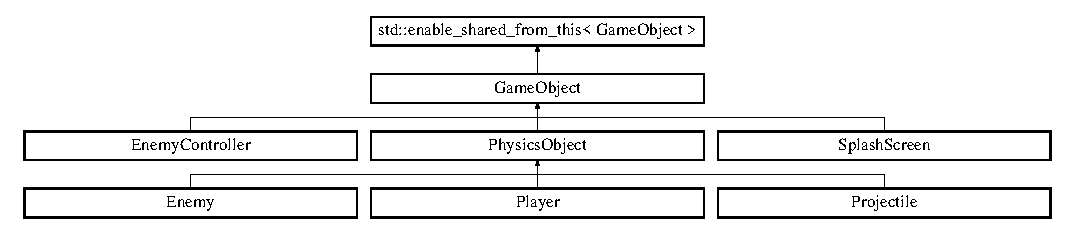
\includegraphics[height=2.021661cm]{d0/dd1/class_game_object}
\end{center}
\end{figure}
\subsection*{Public Member Functions}
\begin{DoxyCompactItemize}
\item 
\mbox{\Hypertarget{class_game_object_a0348e3ee2e83d56eafca7a3547f432c4}\label{class_game_object_a0348e3ee2e83d56eafca7a3547f432c4}} 
\hyperlink{class_game_object_a0348e3ee2e83d56eafca7a3547f432c4}{Game\+Object} ()
\begin{DoxyCompactList}\small\item\em Default Constructor -\/ Creates the object using default values. \end{DoxyCompactList}\item 
\hyperlink{class_game_object_a780db39d3dc5b54c4dffe2f429f9b656}{Game\+Object} (const \hyperlink{class_graphic_object}{Graphic\+Object} \&graphic)
\begin{DoxyCompactList}\small\item\em Constructs an object with a specific \hyperlink{class_graphic_object}{Graphic\+Object}. \end{DoxyCompactList}\item 
\hyperlink{class_game_object_a93186927c126a290592e3d7c13906f18}{Game\+Object} (const \hyperlink{structxy_vector}{xy\+Vector} \&scale)
\begin{DoxyCompactList}\small\item\em Constructs an object with a specific scale. \end{DoxyCompactList}\item 
\hyperlink{class_game_object_a8a9022df605afb6be63d0dcca07667d6}{Game\+Object} (const \hyperlink{class_vector2_d}{Vector2D} \&starting\+Position)
\begin{DoxyCompactList}\small\item\em Constructs an object with a specific starting position. \end{DoxyCompactList}\item 
\mbox{\Hypertarget{class_game_object_adc9ac2a346e947a0dd6f7bd94ecea8af}\label{class_game_object_adc9ac2a346e947a0dd6f7bd94ecea8af}} 
\hyperlink{class_game_object_adc9ac2a346e947a0dd6f7bd94ecea8af}{Game\+Object} (const \hyperlink{class_vector2_d}{Vector2D} \&starting\+Position, const \hyperlink{structxy_vector}{xy\+Vector} \&scale, const \hyperlink{class_graphic_object}{Graphic\+Object} \&graphic\+Object)
\begin{DoxyCompactList}\small\item\em Constructor used to specify the main members of the gameobject. \end{DoxyCompactList}\item 
virtual void \hyperlink{class_game_object_aeeb2162f2779e5591a372a1568bc5c68}{Start} ()
\begin{DoxyCompactList}\small\item\em Used for initialisation of the objects parameters when it is instantiated. \end{DoxyCompactList}\item 
virtual void \hyperlink{class_game_object_ac7ecc123dacaba955077420caabf5e64}{Update} ()
\begin{DoxyCompactList}\small\item\em Update is a virtual method that is used to interface with the Back End System of the Game operations. \end{DoxyCompactList}\item 
bool \hyperlink{class_game_object_a7cc83eeefc6e3d112e2a7fc1fb037a9c}{is\+Active} ()
\begin{DoxyCompactList}\small\item\em get function that allows a client to determine if the \hyperlink{class_game_object}{Game\+Object} is active \end{DoxyCompactList}\item 
\hyperlink{class_vector2_d}{Vector2D} \hyperlink{class_game_object_ae3b21cc28e2c1bce6707699d0312eee8}{get\+Position} () const
\begin{DoxyCompactList}\small\item\em get function used to return the Position of the object, used in the collision\+Detection calculations and the presentation layer \end{DoxyCompactList}\item 
Game\+Object\+Type \hyperlink{class_game_object_af12345846c74b72bc50c779c00b55851}{get\+Type} () const
\begin{DoxyCompactList}\small\item\em get function used to return the Game\+Object\+Type of the object, used in the collision\+Detection calculations \end{DoxyCompactList}\item 
const \hyperlink{structxy_vector}{xy\+Vector} \& \hyperlink{class_game_object_a0e0c63e1c3deedae400d62d3ecab8ef3}{get\+Scale} () const
\begin{DoxyCompactList}\small\item\em get function used to return the scale of the object, used in the presentation layer \end{DoxyCompactList}\item 
virtual const \hyperlink{class_graphic_object}{Graphic\+Object} \& \hyperlink{class_game_object_af44533690a46d5f41aeaa2c16bf867b9}{get\+Graphic\+Object} () const
\begin{DoxyCompactList}\small\item\em Returns the \hyperlink{class_graphic_object}{Graphic\+Object} of the current \hyperlink{class_game_object}{Game\+Object} to interface with the presentation layer. \end{DoxyCompactList}\item 
void \hyperlink{class_game_object_a200218792aa0076011d69be696e3d3d4}{set\+Active} (bool active\+\_\+state)
\begin{DoxyCompactList}\small\item\em Sets the active state of the \hyperlink{class_game_object}{Game\+Object}, if it is unactive it does not update, get displayed by the game or cause collisions. \end{DoxyCompactList}\item 
void \hyperlink{class_game_object_a9e1420c027ce937f9958a41ad280080b}{set\+Scene} (std\+::shared\+\_\+ptr$<$ \hyperlink{class_scene}{Scene} $>$ scene)
\begin{DoxyCompactList}\small\item\em sets the \hyperlink{class_scene}{Scene} pointer of the Gameobject, used to know which \hyperlink{class_scene}{Scene} the \hyperlink{class_game_object}{Game\+Object} exists in \end{DoxyCompactList}\end{DoxyCompactItemize}
\subsection*{Protected Member Functions}
\begin{DoxyCompactItemize}
\item 
std\+::shared\+\_\+ptr$<$ \hyperlink{class_game_object}{Game\+Object} $>$ \hyperlink{class_game_object_ac52291835ad2f3f36363589af0d3ae84}{Find\+Game\+Object\+By\+Type} (Game\+Object\+Type search\+Type)
\begin{DoxyCompactList}\small\item\em Searches the list of available Game\+Objects from the \hyperlink{class_scene}{Scene} object and returns the first object that matches the specifc Game\+Object\+Type. \end{DoxyCompactList}\item 
\mbox{\Hypertarget{class_game_object_abf1959fad10ea04673a182029f1f81b9}\label{class_game_object_abf1959fad10ea04673a182029f1f81b9}} 
void \hyperlink{class_game_object_abf1959fad10ea04673a182029f1f81b9}{Destroy} ()
\begin{DoxyCompactList}\small\item\em Removes the current \hyperlink{class_game_object}{Game\+Object} from the \hyperlink{class_game_object}{Game\+Object} list stored within the current scene. Ensures that the object does not get updated or displayed by the Presentation layer, will be removed from memory once the remaining pointers go out of scope. \end{DoxyCompactList}\end{DoxyCompactItemize}
\subsection*{Protected Attributes}
\begin{DoxyCompactItemize}
\item 
\hyperlink{structxy_vector}{xy\+Vector} \hyperlink{class_game_object_a9b76f90eef67b329538d15b4eeed67a1}{\+\_\+scale}
\item 
std\+::shared\+\_\+ptr$<$ \hyperlink{class_scene}{Scene} $>$ \hyperlink{class_game_object_ab8cae1a41ad1443d085c397b5e6d5609}{\+\_\+scene}
\item 
Game\+Object\+Type \hyperlink{class_game_object_aebfec45400aff20c8eab3fbf00be0aea}{\+\_\+type}
\item 
\hyperlink{class_vector2_d}{Vector2D} \hyperlink{class_game_object_af86156ef21da475d68de98761cf75512}{\+\_\+position}
\item 
\hyperlink{class_graphic_object}{Graphic\+Object} \hyperlink{class_game_object_a07c043ba60b622f256ed18dfb46c0410}{\+\_\+graphic\+Object}
\item 
bool \hyperlink{class_game_object_aef11019578aad93f96240b79a1141a07}{\+\_\+active} = true
\end{DoxyCompactItemize}


\subsection{Detailed Description}
The base class that is used for all game logic systems. 

Gameobject is used as a base class from which the various types of game logic elements are derived from. Every game object exist inside of the game space this invariance means that every game object must have a vector position. The position is used by the Presentation Layer (\hyperlink{class_display_manager}{Display\+Manager}) and the \hyperlink{class_collision_detection}{Collision\+Detection}. \hyperlink{class_game_manager}{Game\+Manager} and \hyperlink{class_scene}{Scene} work together to call the update function for each \hyperlink{class_game_object}{Game\+Object} which acts as the Domain Layer. The virtual functions are overriden by the derived classes to define specific game behaviour. 

\subsection{Constructor \& Destructor Documentation}
\mbox{\Hypertarget{class_game_object_a780db39d3dc5b54c4dffe2f429f9b656}\label{class_game_object_a780db39d3dc5b54c4dffe2f429f9b656}} 
\index{Game\+Object@{Game\+Object}!Game\+Object@{Game\+Object}}
\index{Game\+Object@{Game\+Object}!Game\+Object@{Game\+Object}}
\subsubsection{\texorpdfstring{Game\+Object()}{GameObject()}\hspace{0.1cm}{\footnotesize\ttfamily [1/3]}}
{\footnotesize\ttfamily Game\+Object\+::\+Game\+Object (\begin{DoxyParamCaption}\item[{const \hyperlink{class_graphic_object}{Graphic\+Object} \&}]{graphic }\end{DoxyParamCaption})}



Constructs an object with a specific \hyperlink{class_graphic_object}{Graphic\+Object}. 


\begin{DoxyParams}{Parameters}
{\em graphic} & defines the Game\+Objects \hyperlink{class_graphic_object}{Graphic\+Object} composition \\
\hline
\end{DoxyParams}
\mbox{\Hypertarget{class_game_object_a93186927c126a290592e3d7c13906f18}\label{class_game_object_a93186927c126a290592e3d7c13906f18}} 
\index{Game\+Object@{Game\+Object}!Game\+Object@{Game\+Object}}
\index{Game\+Object@{Game\+Object}!Game\+Object@{Game\+Object}}
\subsubsection{\texorpdfstring{Game\+Object()}{GameObject()}\hspace{0.1cm}{\footnotesize\ttfamily [2/3]}}
{\footnotesize\ttfamily Game\+Object\+::\+Game\+Object (\begin{DoxyParamCaption}\item[{const \hyperlink{structxy_vector}{xy\+Vector} \&}]{scale }\end{DoxyParamCaption})}



Constructs an object with a specific scale. 


\begin{DoxyParams}{Parameters}
{\em scale} & The desired scale for the \hyperlink{class_game_object}{Game\+Object} \\
\hline
\end{DoxyParams}
\mbox{\Hypertarget{class_game_object_a8a9022df605afb6be63d0dcca07667d6}\label{class_game_object_a8a9022df605afb6be63d0dcca07667d6}} 
\index{Game\+Object@{Game\+Object}!Game\+Object@{Game\+Object}}
\index{Game\+Object@{Game\+Object}!Game\+Object@{Game\+Object}}
\subsubsection{\texorpdfstring{Game\+Object()}{GameObject()}\hspace{0.1cm}{\footnotesize\ttfamily [3/3]}}
{\footnotesize\ttfamily Game\+Object\+::\+Game\+Object (\begin{DoxyParamCaption}\item[{const \hyperlink{class_vector2_d}{Vector2D} \&}]{starting\+Position }\end{DoxyParamCaption})}



Constructs an object with a specific starting position. 


\begin{DoxyParams}{Parameters}
{\em starting\+Position} & The desired starting position for the \hyperlink{class_game_object}{Game\+Object} \\
\hline
\end{DoxyParams}


\subsection{Member Function Documentation}
\mbox{\Hypertarget{class_game_object_ac52291835ad2f3f36363589af0d3ae84}\label{class_game_object_ac52291835ad2f3f36363589af0d3ae84}} 
\index{Game\+Object@{Game\+Object}!Find\+Game\+Object\+By\+Type@{Find\+Game\+Object\+By\+Type}}
\index{Find\+Game\+Object\+By\+Type@{Find\+Game\+Object\+By\+Type}!Game\+Object@{Game\+Object}}
\subsubsection{\texorpdfstring{Find\+Game\+Object\+By\+Type()}{FindGameObjectByType()}}
{\footnotesize\ttfamily std\+::shared\+\_\+ptr$<$ \hyperlink{class_game_object}{Game\+Object} $>$ Game\+Object\+::\+Find\+Game\+Object\+By\+Type (\begin{DoxyParamCaption}\item[{Game\+Object\+Type}]{search\+Type }\end{DoxyParamCaption})\hspace{0.3cm}{\ttfamily [protected]}}



Searches the list of available Game\+Objects from the \hyperlink{class_scene}{Scene} object and returns the first object that matches the specifc Game\+Object\+Type. 


\begin{DoxyParams}{Parameters}
{\em search\+Type} & The Game\+Object\+Type that is being searched for, used to find a specific object of a specific type. \\
\hline
\end{DoxyParams}
\begin{DoxyReturn}{Returns}
Returns a pointer to the object of the desired type. 
\end{DoxyReturn}
\mbox{\Hypertarget{class_game_object_af44533690a46d5f41aeaa2c16bf867b9}\label{class_game_object_af44533690a46d5f41aeaa2c16bf867b9}} 
\index{Game\+Object@{Game\+Object}!get\+Graphic\+Object@{get\+Graphic\+Object}}
\index{get\+Graphic\+Object@{get\+Graphic\+Object}!Game\+Object@{Game\+Object}}
\subsubsection{\texorpdfstring{get\+Graphic\+Object()}{getGraphicObject()}}
{\footnotesize\ttfamily const \hyperlink{class_graphic_object}{Graphic\+Object} \& Game\+Object\+::get\+Graphic\+Object (\begin{DoxyParamCaption}{ }\end{DoxyParamCaption}) const\hspace{0.3cm}{\ttfamily [virtual]}}



Returns the \hyperlink{class_graphic_object}{Graphic\+Object} of the current \hyperlink{class_game_object}{Game\+Object} to interface with the presentation layer. 

\begin{DoxyReturn}{Returns}
Returns the \hyperlink{class_graphic_object}{Graphic\+Object} composition object 
\end{DoxyReturn}
\mbox{\Hypertarget{class_game_object_ae3b21cc28e2c1bce6707699d0312eee8}\label{class_game_object_ae3b21cc28e2c1bce6707699d0312eee8}} 
\index{Game\+Object@{Game\+Object}!get\+Position@{get\+Position}}
\index{get\+Position@{get\+Position}!Game\+Object@{Game\+Object}}
\subsubsection{\texorpdfstring{get\+Position()}{getPosition()}}
{\footnotesize\ttfamily \hyperlink{class_vector2_d}{Vector2D} Game\+Object\+::get\+Position (\begin{DoxyParamCaption}{ }\end{DoxyParamCaption}) const\hspace{0.3cm}{\ttfamily [inline]}}



get function used to return the Position of the object, used in the collision\+Detection calculations and the presentation layer 

\begin{DoxyReturn}{Returns}
Returns the \hyperlink{class_vector2_d}{Vector2D} composition object 
\end{DoxyReturn}
\mbox{\Hypertarget{class_game_object_a0e0c63e1c3deedae400d62d3ecab8ef3}\label{class_game_object_a0e0c63e1c3deedae400d62d3ecab8ef3}} 
\index{Game\+Object@{Game\+Object}!get\+Scale@{get\+Scale}}
\index{get\+Scale@{get\+Scale}!Game\+Object@{Game\+Object}}
\subsubsection{\texorpdfstring{get\+Scale()}{getScale()}}
{\footnotesize\ttfamily const \hyperlink{structxy_vector}{xy\+Vector}\& Game\+Object\+::get\+Scale (\begin{DoxyParamCaption}{ }\end{DoxyParamCaption}) const\hspace{0.3cm}{\ttfamily [inline]}}



get function used to return the scale of the object, used in the presentation layer 

\begin{DoxyReturn}{Returns}
Returns the \hyperlink{structxy_vector}{xy\+Vector} composition object 
\end{DoxyReturn}
\mbox{\Hypertarget{class_game_object_af12345846c74b72bc50c779c00b55851}\label{class_game_object_af12345846c74b72bc50c779c00b55851}} 
\index{Game\+Object@{Game\+Object}!get\+Type@{get\+Type}}
\index{get\+Type@{get\+Type}!Game\+Object@{Game\+Object}}
\subsubsection{\texorpdfstring{get\+Type()}{getType()}}
{\footnotesize\ttfamily Game\+Object\+Type Game\+Object\+::get\+Type (\begin{DoxyParamCaption}{ }\end{DoxyParamCaption}) const\hspace{0.3cm}{\ttfamily [inline]}}



get function used to return the Game\+Object\+Type of the object, used in the collision\+Detection calculations 

\begin{DoxyReturn}{Returns}
Returns the \hyperlink{structxy_vector}{xy\+Vector} composition object 
\end{DoxyReturn}
\mbox{\Hypertarget{class_game_object_a7cc83eeefc6e3d112e2a7fc1fb037a9c}\label{class_game_object_a7cc83eeefc6e3d112e2a7fc1fb037a9c}} 
\index{Game\+Object@{Game\+Object}!is\+Active@{is\+Active}}
\index{is\+Active@{is\+Active}!Game\+Object@{Game\+Object}}
\subsubsection{\texorpdfstring{is\+Active()}{isActive()}}
{\footnotesize\ttfamily bool Game\+Object\+::is\+Active (\begin{DoxyParamCaption}{ }\end{DoxyParamCaption})\hspace{0.3cm}{\ttfamily [inline]}}



get function that allows a client to determine if the \hyperlink{class_game_object}{Game\+Object} is active 

\begin{DoxyReturn}{Returns}
Returns the boolean that represents the Game\+Objects active state 
\end{DoxyReturn}
\mbox{\Hypertarget{class_game_object_a200218792aa0076011d69be696e3d3d4}\label{class_game_object_a200218792aa0076011d69be696e3d3d4}} 
\index{Game\+Object@{Game\+Object}!set\+Active@{set\+Active}}
\index{set\+Active@{set\+Active}!Game\+Object@{Game\+Object}}
\subsubsection{\texorpdfstring{set\+Active()}{setActive()}}
{\footnotesize\ttfamily void Game\+Object\+::set\+Active (\begin{DoxyParamCaption}\item[{bool}]{active\+\_\+state }\end{DoxyParamCaption})\hspace{0.3cm}{\ttfamily [inline]}}



Sets the active state of the \hyperlink{class_game_object}{Game\+Object}, if it is unactive it does not update, get displayed by the game or cause collisions. 


\begin{DoxyParams}{Parameters}
{\em active\+\_\+state} & the desired state of the Gameobject \\
\hline
\end{DoxyParams}
\mbox{\Hypertarget{class_game_object_a9e1420c027ce937f9958a41ad280080b}\label{class_game_object_a9e1420c027ce937f9958a41ad280080b}} 
\index{Game\+Object@{Game\+Object}!set\+Scene@{set\+Scene}}
\index{set\+Scene@{set\+Scene}!Game\+Object@{Game\+Object}}
\subsubsection{\texorpdfstring{set\+Scene()}{setScene()}}
{\footnotesize\ttfamily void Game\+Object\+::set\+Scene (\begin{DoxyParamCaption}\item[{std\+::shared\+\_\+ptr$<$ \hyperlink{class_scene}{Scene} $>$}]{scene }\end{DoxyParamCaption})\hspace{0.3cm}{\ttfamily [inline]}}



sets the \hyperlink{class_scene}{Scene} pointer of the Gameobject, used to know which \hyperlink{class_scene}{Scene} the \hyperlink{class_game_object}{Game\+Object} exists in 


\begin{DoxyParams}{Parameters}
{\em scene} & The \hyperlink{class_scene}{Scene} pointer that is copied \\
\hline
\end{DoxyParams}
\mbox{\Hypertarget{class_game_object_aeeb2162f2779e5591a372a1568bc5c68}\label{class_game_object_aeeb2162f2779e5591a372a1568bc5c68}} 
\index{Game\+Object@{Game\+Object}!Start@{Start}}
\index{Start@{Start}!Game\+Object@{Game\+Object}}
\subsubsection{\texorpdfstring{Start()}{Start()}}
{\footnotesize\ttfamily virtual void Game\+Object\+::\+Start (\begin{DoxyParamCaption}{ }\end{DoxyParamCaption})\hspace{0.3cm}{\ttfamily [inline]}, {\ttfamily [virtual]}}



Used for initialisation of the objects parameters when it is instantiated. 

Start is used to define the various intitialisation parameters that an object may require to be set before it exists inside of the game scene. The \hyperlink{class_scene}{Scene} Object calls this function when it is instantiated 

Reimplemented in \hyperlink{class_enemy_a64ee0cc6fb8a3424d486537efb8205d8}{Enemy}, \hyperlink{class_projectile_a27a59059730a66a37feec766ebe08fa2}{Projectile}, and \hyperlink{class_laser_generator_container_a9fc676b255f742a97ec0eb6036491684}{Laser\+Generator\+Container}.

\mbox{\Hypertarget{class_game_object_ac7ecc123dacaba955077420caabf5e64}\label{class_game_object_ac7ecc123dacaba955077420caabf5e64}} 
\index{Game\+Object@{Game\+Object}!Update@{Update}}
\index{Update@{Update}!Game\+Object@{Game\+Object}}
\subsubsection{\texorpdfstring{Update()}{Update()}}
{\footnotesize\ttfamily virtual void Game\+Object\+::\+Update (\begin{DoxyParamCaption}{ }\end{DoxyParamCaption})\hspace{0.3cm}{\ttfamily [inline]}, {\ttfamily [virtual]}}



Update is a virtual method that is used to interface with the Back End System of the Game operations. 

Update is managed by the scene object which iterates through the list of Game\+Objects composed within it. For each \hyperlink{class_game_object}{Game\+Object} the Update function is called once per frame. This function is overriden by the various derived classes, it is given a default return that does nothing, this enables derived classes to implement it only when necessary. 

Reimplemented in \hyperlink{class_enemy_a614ad271f07ecf63cb3e665155b7e258}{Enemy}, \hyperlink{class_projectile_a1f9df5dd65fed410d4e897eb63edc1c9}{Projectile}, \hyperlink{class_enemy_controller_af36ec67442d30c7519581b83ad6c00db}{Enemy\+Controller}, \hyperlink{class_player_a5e17be3418fa0ac0192c05efaf3dc8bd}{Player}, and \hyperlink{class_splash_screen_af78b8eab226a89fec389e53cbf3ed9e8}{Splash\+Screen}.



\subsection{Member Data Documentation}
\mbox{\Hypertarget{class_game_object_aef11019578aad93f96240b79a1141a07}\label{class_game_object_aef11019578aad93f96240b79a1141a07}} 
\index{Game\+Object@{Game\+Object}!\+\_\+active@{\+\_\+active}}
\index{\+\_\+active@{\+\_\+active}!Game\+Object@{Game\+Object}}
\subsubsection{\texorpdfstring{\+\_\+active}{\_active}}
{\footnotesize\ttfamily bool Game\+Object\+::\+\_\+active = true\hspace{0.3cm}{\ttfamily [protected]}}

Returns the active state of the object, does not get displayed or updated when not active \mbox{\Hypertarget{class_game_object_a07c043ba60b622f256ed18dfb46c0410}\label{class_game_object_a07c043ba60b622f256ed18dfb46c0410}} 
\index{Game\+Object@{Game\+Object}!\+\_\+graphic\+Object@{\+\_\+graphic\+Object}}
\index{\+\_\+graphic\+Object@{\+\_\+graphic\+Object}!Game\+Object@{Game\+Object}}
\subsubsection{\texorpdfstring{\+\_\+graphic\+Object}{\_graphicObject}}
{\footnotesize\ttfamily \hyperlink{class_graphic_object}{Graphic\+Object} Game\+Object\+::\+\_\+graphic\+Object\hspace{0.3cm}{\ttfamily [protected]}}

The \hyperlink{class_graphic_object}{Graphic\+Object} composition used to identify the specific Sprite the \hyperlink{class_game_object}{Game\+Object} \mbox{\Hypertarget{class_game_object_af86156ef21da475d68de98761cf75512}\label{class_game_object_af86156ef21da475d68de98761cf75512}} 
\index{Game\+Object@{Game\+Object}!\+\_\+position@{\+\_\+position}}
\index{\+\_\+position@{\+\_\+position}!Game\+Object@{Game\+Object}}
\subsubsection{\texorpdfstring{\+\_\+position}{\_position}}
{\footnotesize\ttfamily \hyperlink{class_vector2_d}{Vector2D} Game\+Object\+::\+\_\+position\hspace{0.3cm}{\ttfamily [protected]}}

The \hyperlink{class_vector2_d}{Vector2D} composition used to represent the objects position in the game\textquotesingle{}s Vector space \mbox{\Hypertarget{class_game_object_a9b76f90eef67b329538d15b4eeed67a1}\label{class_game_object_a9b76f90eef67b329538d15b4eeed67a1}} 
\index{Game\+Object@{Game\+Object}!\+\_\+scale@{\+\_\+scale}}
\index{\+\_\+scale@{\+\_\+scale}!Game\+Object@{Game\+Object}}
\subsubsection{\texorpdfstring{\+\_\+scale}{\_scale}}
{\footnotesize\ttfamily \hyperlink{structxy_vector}{xy\+Vector} Game\+Object\+::\+\_\+scale\hspace{0.3cm}{\ttfamily [protected]}}

\hyperlink{structxy_vector}{xy\+Vector} representing the scale of the object \mbox{\Hypertarget{class_game_object_ab8cae1a41ad1443d085c397b5e6d5609}\label{class_game_object_ab8cae1a41ad1443d085c397b5e6d5609}} 
\index{Game\+Object@{Game\+Object}!\+\_\+scene@{\+\_\+scene}}
\index{\+\_\+scene@{\+\_\+scene}!Game\+Object@{Game\+Object}}
\subsubsection{\texorpdfstring{\+\_\+scene}{\_scene}}
{\footnotesize\ttfamily std\+::shared\+\_\+ptr$<$\hyperlink{class_scene}{Scene}$>$ Game\+Object\+::\+\_\+scene\hspace{0.3cm}{\ttfamily [protected]}}

The \hyperlink{class_scene}{Scene} that the object exists in \mbox{\Hypertarget{class_game_object_aebfec45400aff20c8eab3fbf00be0aea}\label{class_game_object_aebfec45400aff20c8eab3fbf00be0aea}} 
\index{Game\+Object@{Game\+Object}!\+\_\+type@{\+\_\+type}}
\index{\+\_\+type@{\+\_\+type}!Game\+Object@{Game\+Object}}
\subsubsection{\texorpdfstring{\+\_\+type}{\_type}}
{\footnotesize\ttfamily Game\+Object\+Type Game\+Object\+::\+\_\+type\hspace{0.3cm}{\ttfamily [protected]}}

The Game\+Object\+Type representation of the object 

The documentation for this class was generated from the following files\+:\begin{DoxyCompactItemize}
\item 
C\+:/\+Users/\+Tim/\+Documents/\+Software\+Dev/\+Software\+Project/\+Project\+Files/game-\/source-\/code/\+Front\+End\+Systems/Game\+Object.\+h\item 
C\+:/\+Users/\+Tim/\+Documents/\+Software\+Dev/\+Software\+Project/\+Project\+Files/game-\/source-\/code/\+Front\+End\+Systems/Game\+Object.\+cpp\end{DoxyCompactItemize}

\hypertarget{class_game_time}{}\section{Game\+Time Class Reference}
\label{class_game_time}\index{Game\+Time@{Game\+Time}}


Determines the time that it takes for a single frame.  




{\ttfamily \#include $<$Game\+Time.\+h$>$}

\subsection*{Public Member Functions}
\begin{DoxyCompactItemize}
\item 
\mbox{\Hypertarget{class_game_time_ab3b7fbfbc2a94e223d349b3dd48f76d3}\label{class_game_time_ab3b7fbfbc2a94e223d349b3dd48f76d3}} 
\hyperlink{class_game_time_ab3b7fbfbc2a94e223d349b3dd48f76d3}{Game\+Time} ()
\begin{DoxyCompactList}\small\item\em Constructs the \hyperlink{class_game_time}{Game\+Time} object and seeds the random generator. \end{DoxyCompactList}\item 
\mbox{\Hypertarget{class_game_time_a424d4e2f4745a85897620751ff5153b9}\label{class_game_time_a424d4e2f4745a85897620751ff5153b9}} 
void \hyperlink{class_game_time_a424d4e2f4745a85897620751ff5153b9}{Time\+Frame} ()
\begin{DoxyCompactList}\small\item\em Times the current frame and determines the new delta time. \end{DoxyCompactList}\end{DoxyCompactItemize}
\subsection*{Static Public Member Functions}
\begin{DoxyCompactItemize}
\item 
static double \hyperlink{class_game_time_aa5ea84c887116ef68d1331617c5a81c3}{get\+Delta\+Time} ()
\begin{DoxyCompactList}\small\item\em Returns the difference in time between the last frame and the current frame. \end{DoxyCompactList}\end{DoxyCompactItemize}
\subsection*{Private Member Functions}
\begin{DoxyCompactItemize}
\item 
double \hyperlink{class_game_time_ac8a380f740f5bc39e98fda3e069c0bb3}{calc\+Process\+Time} ()
\begin{DoxyCompactList}\small\item\em Determines the amount of time that has passes since the game began running, converts it into a double and returns the value. \end{DoxyCompactList}\item 
\mbox{\Hypertarget{class_game_time_a8575cb09f1e07b90678eedaf92776a97}\label{class_game_time_a8575cb09f1e07b90678eedaf92776a97}} 
void \hyperlink{class_game_time_a8575cb09f1e07b90678eedaf92776a97}{calc\+Delta\+Time} ()
\begin{DoxyCompactList}\small\item\em Calculates the time between the current frame and the last frame. \end{DoxyCompactList}\item 
\mbox{\Hypertarget{class_game_time_aec3fa5e495f783524701418f5d679071}\label{class_game_time_aec3fa5e495f783524701418f5d679071}} 
void \hyperlink{class_game_time_aec3fa5e495f783524701418f5d679071}{calc\+Current\+Time} ()
\begin{DoxyCompactList}\small\item\em Calculates the time up until the current frame. \end{DoxyCompactList}\end{DoxyCompactItemize}
\subsection*{Static Private Attributes}
\begin{DoxyCompactItemize}
\item 
static double \hyperlink{class_game_time_a080d9deb72c675f0d68f9ad72eec66c3}{\+\_\+current\+\_\+time} = 0
\begin{DoxyCompactList}\small\item\em variables and names need to be changed to make it more understandable \end{DoxyCompactList}\item 
static double \hyperlink{class_game_time_a39c7a52db277a99fd6dfcb457b432d7d}{\+\_\+delta\+Time} = 1
\end{DoxyCompactItemize}


\subsection{Detailed Description}
Determines the time that it takes for a single frame. 

Used to create smooth interactions between the Game logic and the Back\+End\+Systems 

\subsection{Member Function Documentation}
\mbox{\Hypertarget{class_game_time_ac8a380f740f5bc39e98fda3e069c0bb3}\label{class_game_time_ac8a380f740f5bc39e98fda3e069c0bb3}} 
\index{Game\+Time@{Game\+Time}!calc\+Process\+Time@{calc\+Process\+Time}}
\index{calc\+Process\+Time@{calc\+Process\+Time}!Game\+Time@{Game\+Time}}
\subsubsection{\texorpdfstring{calc\+Process\+Time()}{calcProcessTime()}}
{\footnotesize\ttfamily double Game\+Time\+::calc\+Process\+Time (\begin{DoxyParamCaption}{ }\end{DoxyParamCaption})\hspace{0.3cm}{\ttfamily [private]}}



Determines the amount of time that has passes since the game began running, converts it into a double and returns the value. 

\begin{DoxyReturn}{Returns}
Returns the amount of time that has passed since the game began 
\end{DoxyReturn}
\mbox{\Hypertarget{class_game_time_aa5ea84c887116ef68d1331617c5a81c3}\label{class_game_time_aa5ea84c887116ef68d1331617c5a81c3}} 
\index{Game\+Time@{Game\+Time}!get\+Delta\+Time@{get\+Delta\+Time}}
\index{get\+Delta\+Time@{get\+Delta\+Time}!Game\+Time@{Game\+Time}}
\subsubsection{\texorpdfstring{get\+Delta\+Time()}{getDeltaTime()}}
{\footnotesize\ttfamily double Game\+Time\+::get\+Delta\+Time (\begin{DoxyParamCaption}{ }\end{DoxyParamCaption})\hspace{0.3cm}{\ttfamily [static]}}



Returns the difference in time between the last frame and the current frame. 

\begin{DoxyReturn}{Returns}
Returns the difference in time between the last frame and the current frame 
\end{DoxyReturn}


\subsection{Member Data Documentation}
\mbox{\Hypertarget{class_game_time_a080d9deb72c675f0d68f9ad72eec66c3}\label{class_game_time_a080d9deb72c675f0d68f9ad72eec66c3}} 
\index{Game\+Time@{Game\+Time}!\+\_\+current\+\_\+time@{\+\_\+current\+\_\+time}}
\index{\+\_\+current\+\_\+time@{\+\_\+current\+\_\+time}!Game\+Time@{Game\+Time}}
\subsubsection{\texorpdfstring{\+\_\+current\+\_\+time}{\_current\_time}}
{\footnotesize\ttfamily double Game\+Time\+::\+\_\+current\+\_\+time = 0\hspace{0.3cm}{\ttfamily [static]}, {\ttfamily [private]}}



variables and names need to be changed to make it more understandable 

current time up till the current frame \mbox{\Hypertarget{class_game_time_a39c7a52db277a99fd6dfcb457b432d7d}\label{class_game_time_a39c7a52db277a99fd6dfcb457b432d7d}} 
\index{Game\+Time@{Game\+Time}!\+\_\+delta\+Time@{\+\_\+delta\+Time}}
\index{\+\_\+delta\+Time@{\+\_\+delta\+Time}!Game\+Time@{Game\+Time}}
\subsubsection{\texorpdfstring{\+\_\+delta\+Time}{\_deltaTime}}
{\footnotesize\ttfamily double Game\+Time\+::\+\_\+delta\+Time = 1\hspace{0.3cm}{\ttfamily [static]}, {\ttfamily [private]}}

change in time between frames 

The documentation for this class was generated from the following files\+:\begin{DoxyCompactItemize}
\item 
D\+:/\+Users/\+Tim-\/\+P\+C/\+Documents/\+Software\+\_\+\+I\+I/\+Project/\+Project\+Files/game-\/source-\/code/\+Back\+End\+Systems/Game\+Time.\+h\item 
D\+:/\+Users/\+Tim-\/\+P\+C/\+Documents/\+Software\+\_\+\+I\+I/\+Project/\+Project\+Files/game-\/source-\/code/\+Back\+End\+Systems/Game\+Time.\+cpp\end{DoxyCompactItemize}

\hypertarget{class_graphic_name_reservedfoo_null_graphic}{}\section{Graphic\+Name\+Reservedfoo\+Null\+Graphic Class Reference}
\label{class_graphic_name_reservedfoo_null_graphic}\index{Graphic\+Name\+Reservedfoo\+Null\+Graphic@{Graphic\+Name\+Reservedfoo\+Null\+Graphic}}


Exception thrown when the client attempts to create an object with the same \+\_\+graphic\+Name as the Null\+Graphics.  




\subsection{Detailed Description}
Exception thrown when the client attempts to create an object with the same \+\_\+graphic\+Name as the Null\+Graphics. 

The documentation for this class was generated from the following file\+:\begin{DoxyCompactItemize}
\item 
D\+:/\+Users/\+Tim-\/\+P\+C/\+Documents/\+Software\+\_\+\+I\+I/\+Project/\+Project\+Files/game-\/source-\/code/\+Front\+End\+Systems/Graphic\+Object.\+cpp\end{DoxyCompactItemize}

\hypertarget{class_graphic_name_reservedfor_null_graphic}{}\section{Graphic\+Name\+Reservedfor\+Null\+Graphic Class Reference}
\label{class_graphic_name_reservedfor_null_graphic}\index{Graphic\+Name\+Reservedfor\+Null\+Graphic@{Graphic\+Name\+Reservedfor\+Null\+Graphic}}


The documentation for this class was generated from the following file\+:\begin{DoxyCompactItemize}
\item 
D\+:/\+Users/\+Tim-\/\+P\+C/\+Documents/\+Software\+\_\+\+I\+I/\+Project/\+Project\+Files/game-\/source-\/code/\+Front\+End\+Systems/Graphic\+Object.\+cpp\end{DoxyCompactItemize}

\hypertarget{class_graphic_object}{}\section{Graphic\+Object Class Reference}
\label{class_graphic_object}\index{Graphic\+Object@{Graphic\+Object}}


This is the Utility class with the display manager, It stores the name of the object and location of the image file which are both necessary for the \hyperlink{class_display_manager}{Display\+Manager} to correctly display the specified image.  




{\ttfamily \#include $<$Graphic\+Object.\+h$>$}

\subsection*{Public Member Functions}
\begin{DoxyCompactItemize}
\item 
\mbox{\Hypertarget{class_graphic_object_ae1b56ae4484ad120f5ba77c0b683a045}\label{class_graphic_object_ae1b56ae4484ad120f5ba77c0b683a045}} 
\hyperlink{class_graphic_object_ae1b56ae4484ad120f5ba77c0b683a045}{Graphic\+Object} ()
\begin{DoxyCompactList}\small\item\em Default Constructor, creates a Null\+Graphic by default. \end{DoxyCompactList}\item 
\mbox{\Hypertarget{class_graphic_object_a4a14ca7f3b9e9736b0b4231ee08dc0ab}\label{class_graphic_object_a4a14ca7f3b9e9736b0b4231ee08dc0ab}} 
\hyperlink{class_graphic_object_a4a14ca7f3b9e9736b0b4231ee08dc0ab}{Graphic\+Object} (const \hyperlink{class_graphic_object}{Graphic\+Object} \&copy)
\begin{DoxyCompactList}\small\item\em Copy Constructor of \hyperlink{class_graphic_object}{Graphic\+Object}. \end{DoxyCompactList}\item 
\mbox{\Hypertarget{class_graphic_object_a4026dc4e922a5053b6c0e3d1a9b28b63}\label{class_graphic_object_a4026dc4e922a5053b6c0e3d1a9b28b63}} 
\hyperlink{class_graphic_object}{Graphic\+Object} \& \hyperlink{class_graphic_object_a4026dc4e922a5053b6c0e3d1a9b28b63}{operator=} (const \hyperlink{class_graphic_object}{Graphic\+Object} \&rhs)
\begin{DoxyCompactList}\small\item\em Assignment operator overload. \end{DoxyCompactList}\item 
\hyperlink{class_graphic_object_a9819ca0b4c1bb72ede070d8485bfc8a9}{Graphic\+Object} (string texture\+Location, string graphic\+Name)
\begin{DoxyCompactList}\small\item\em Standard Constructor, creates a Graphic Object with the client specified parameters. \end{DoxyCompactList}\item 
const string \& \hyperlink{class_graphic_object_a8772813296b837e997ee21836e92b028}{get\+Graphic\+Name} () const
\begin{DoxyCompactList}\small\item\em Getter is necessary to decouple the presentation layer from the game logic layer. \end{DoxyCompactList}\item 
const string \& \hyperlink{class_graphic_object_a1041a2dd82f82fc724675c5a2ea67d32}{get\+Texture\+Location} () const
\begin{DoxyCompactList}\small\item\em Getter is necessary to decouple the presentation layer from the game logic layer. \end{DoxyCompactList}\end{DoxyCompactItemize}
\subsection*{Static Public Attributes}
\begin{DoxyCompactItemize}
\item 
\mbox{\Hypertarget{class_graphic_object_a3a6832e8f4af96da2935d3c69757107c}\label{class_graphic_object_a3a6832e8f4af96da2935d3c69757107c}} 
static const \hyperlink{class_graphic_object}{Graphic\+Object} \hyperlink{class_graphic_object_a3a6832e8f4af96da2935d3c69757107c}{Null\+Graphic} \{\char`\"{}Null\char`\"{}, \char`\"{}Null\+Graphic.\+png\char`\"{}\}
\begin{DoxyCompactList}\small\item\em Null\+Graphic Declaration, requires the \char`\"{}\+Null\+Graphic.\+png\char`\"{} image to be available. \end{DoxyCompactList}\end{DoxyCompactItemize}
\subsection*{Protected Attributes}
\begin{DoxyCompactItemize}
\item 
std\+::string \hyperlink{class_graphic_object_a3fc571887a6e46dda4a4ef10d44720b5}{\+\_\+texture\+Location}
\item 
std\+::string \hyperlink{class_graphic_object_a74c9292d37d9be9e099c868be084b33f}{\+\_\+graphic\+Name}
\end{DoxyCompactItemize}


\subsection{Detailed Description}
This is the Utility class with the display manager, It stores the name of the object and location of the image file which are both necessary for the \hyperlink{class_display_manager}{Display\+Manager} to correctly display the specified image. 

The Graphic Object has a tight coupling with the Presentation layer classes. The graphic name of the object is used as a key within a hashtable to identify the specific sfml sprite and texture that needs to be drawn for the corresponding object. \hyperlink{class_graphic_object}{Graphic\+Object} acts as a link between the Presentation Layer and the Domain layer. It forms a composition relationship with the \hyperlink{class_game_object}{Game\+Object} class. A Null\+Object is assigned by default for derived implimentations of \hyperlink{class_game_object}{Game\+Object} that do not require a \hyperlink{class_graphic_object}{Graphic\+Object} The Null\+Object consistis of a Null\+Object.\+png image which is a single transparent pixel and the graphic\+Name Null. This is an Object name that is preserved by the constructor. ie another \hyperlink{class_graphic_object}{Graphic\+Object} may not have the name Null. 

\subsection{Constructor \& Destructor Documentation}
\mbox{\Hypertarget{class_graphic_object_a9819ca0b4c1bb72ede070d8485bfc8a9}\label{class_graphic_object_a9819ca0b4c1bb72ede070d8485bfc8a9}} 
\index{Graphic\+Object@{Graphic\+Object}!Graphic\+Object@{Graphic\+Object}}
\index{Graphic\+Object@{Graphic\+Object}!Graphic\+Object@{Graphic\+Object}}
\subsubsection{\texorpdfstring{Graphic\+Object()}{GraphicObject()}}
{\footnotesize\ttfamily Graphic\+Object\+::\+Graphic\+Object (\begin{DoxyParamCaption}\item[{string}]{texture\+Location,  }\item[{string}]{graphic\+Name }\end{DoxyParamCaption})}



Standard Constructor, creates a Graphic Object with the client specified parameters. 


\begin{DoxyParams}{Parameters}
{\em texture\+Location} & The texture location for the image that the object uses \\
\hline
{\em graphic\+Name} & The name of that corresponds to objects that use the same image\\
\hline
\end{DoxyParams}
Checks if the reserved graphic\+Name \char`\"{}\+Null\char`\"{} is used, throws \hyperlink{class_graphic_name_reservedfor_null_graphic}{Graphic\+Name\+Reservedfor\+Null\+Graphic} if Null is used 

\subsection{Member Function Documentation}
\mbox{\Hypertarget{class_graphic_object_a8772813296b837e997ee21836e92b028}\label{class_graphic_object_a8772813296b837e997ee21836e92b028}} 
\index{Graphic\+Object@{Graphic\+Object}!get\+Graphic\+Name@{get\+Graphic\+Name}}
\index{get\+Graphic\+Name@{get\+Graphic\+Name}!Graphic\+Object@{Graphic\+Object}}
\subsubsection{\texorpdfstring{get\+Graphic\+Name()}{getGraphicName()}}
{\footnotesize\ttfamily const string\& Graphic\+Object\+::get\+Graphic\+Name (\begin{DoxyParamCaption}{ }\end{DoxyParamCaption}) const\hspace{0.3cm}{\ttfamily [inline]}}



Getter is necessary to decouple the presentation layer from the game logic layer. 

\begin{DoxyReturn}{Returns}
Returns a constant string that represents the graphic name of the object 
\end{DoxyReturn}
\mbox{\Hypertarget{class_graphic_object_a1041a2dd82f82fc724675c5a2ea67d32}\label{class_graphic_object_a1041a2dd82f82fc724675c5a2ea67d32}} 
\index{Graphic\+Object@{Graphic\+Object}!get\+Texture\+Location@{get\+Texture\+Location}}
\index{get\+Texture\+Location@{get\+Texture\+Location}!Graphic\+Object@{Graphic\+Object}}
\subsubsection{\texorpdfstring{get\+Texture\+Location()}{getTextureLocation()}}
{\footnotesize\ttfamily const string\& Graphic\+Object\+::get\+Texture\+Location (\begin{DoxyParamCaption}{ }\end{DoxyParamCaption}) const\hspace{0.3cm}{\ttfamily [inline]}}



Getter is necessary to decouple the presentation layer from the game logic layer. 

\begin{DoxyReturn}{Returns}
Returns a constant string that represents the location of the image file that is being used 
\end{DoxyReturn}


\subsection{Member Data Documentation}
\mbox{\Hypertarget{class_graphic_object_a74c9292d37d9be9e099c868be084b33f}\label{class_graphic_object_a74c9292d37d9be9e099c868be084b33f}} 
\index{Graphic\+Object@{Graphic\+Object}!\+\_\+graphic\+Name@{\+\_\+graphic\+Name}}
\index{\+\_\+graphic\+Name@{\+\_\+graphic\+Name}!Graphic\+Object@{Graphic\+Object}}
\subsubsection{\texorpdfstring{\+\_\+graphic\+Name}{\_graphicName}}
{\footnotesize\ttfamily std\+::string Graphic\+Object\+::\+\_\+graphic\+Name\hspace{0.3cm}{\ttfamily [protected]}}

The name used to load objects specified by the texture location$>$ \mbox{\Hypertarget{class_graphic_object_a3fc571887a6e46dda4a4ef10d44720b5}\label{class_graphic_object_a3fc571887a6e46dda4a4ef10d44720b5}} 
\index{Graphic\+Object@{Graphic\+Object}!\+\_\+texture\+Location@{\+\_\+texture\+Location}}
\index{\+\_\+texture\+Location@{\+\_\+texture\+Location}!Graphic\+Object@{Graphic\+Object}}
\subsubsection{\texorpdfstring{\+\_\+texture\+Location}{\_textureLocation}}
{\footnotesize\ttfamily std\+::string Graphic\+Object\+::\+\_\+texture\+Location\hspace{0.3cm}{\ttfamily [protected]}}

The location of the Image that the object represents$>$ 

The documentation for this class was generated from the following files\+:\begin{DoxyCompactItemize}
\item 
D\+:/\+Users/\+Tim-\/\+P\+C/\+Documents/\+Software\+\_\+\+I\+I/\+Project/\+Project\+Files/game-\/source-\/code/\+Front\+End\+Systems/Graphic\+Object.\+h\item 
D\+:/\+Users/\+Tim-\/\+P\+C/\+Documents/\+Software\+\_\+\+I\+I/\+Project/\+Project\+Files/game-\/source-\/code/\+Front\+End\+Systems/Graphic\+Object.\+cpp\end{DoxyCompactItemize}

\hypertarget{class_input}{}\section{Input Class Reference}
\label{class_input}\index{Input@{Input}}


Responsible for supplying the Front\+End\+System with access to the input of the user by interfaceing with sfml.  




{\ttfamily \#include $<$Input.\+h$>$}

\subsection*{Static Public Member Functions}
\begin{DoxyCompactItemize}
\item 
static bool \hyperlink{class_input_abb8551549ffe7b1474aca91ce3509d57}{Is\+Button\+Pressed} (Keys key)
\begin{DoxyCompactList}\small\item\em returns a boolean for the specific key that is pressed , returns true if the Key has been pressed \end{DoxyCompactList}\item 
static int \hyperlink{class_input_a5c4b1c67c7d3e28d4af79601c81ed8bb}{get\+Axis} (Axis axis)
\begin{DoxyCompactList}\small\item\em Provides directional information inherintly,. \end{DoxyCompactList}\item 
static void \hyperlink{class_input_a851f7b43b30dcf7166af7c548d21316f}{set\+Button} (Keys key, bool state)
\begin{DoxyCompactList}\small\item\em Sets the specific Key to the desired state of whether it is pressed or not. \end{DoxyCompactList}\end{DoxyCompactItemize}
\subsection*{Static Private Member Functions}
\begin{DoxyCompactItemize}
\item 
static int \hyperlink{class_input_a7419956b2d6001cef104b8abdf242477}{Check\+Button\+For\+Axis} (Keys negative\+Key, Keys positive\+Key)
\end{DoxyCompactItemize}
\subsection*{Static Private Attributes}
\begin{DoxyCompactItemize}
\item 
static std\+::vector$<$ bool $>$ \hyperlink{class_input_affef708e1d603d97a7218b64eab063b5}{\+\_\+buttons}
\end{DoxyCompactItemize}


\subsection{Detailed Description}
Responsible for supplying the Front\+End\+System with access to the input of the user by interfaceing with sfml. 

\subsection{Member Function Documentation}
\mbox{\Hypertarget{class_input_a7419956b2d6001cef104b8abdf242477}\label{class_input_a7419956b2d6001cef104b8abdf242477}} 
\index{Input@{Input}!Check\+Button\+For\+Axis@{Check\+Button\+For\+Axis}}
\index{Check\+Button\+For\+Axis@{Check\+Button\+For\+Axis}!Input@{Input}}
\subsubsection{\texorpdfstring{Check\+Button\+For\+Axis()}{CheckButtonForAxis()}}
{\footnotesize\ttfamily int Input\+::\+Check\+Button\+For\+Axis (\begin{DoxyParamCaption}\item[{Keys}]{negative\+Key,  }\item[{Keys}]{positive\+Key }\end{DoxyParamCaption})\hspace{0.3cm}{\ttfamily [static]}, {\ttfamily [private]}}

Uses the buttons to determine direction from button presses \mbox{\Hypertarget{class_input_a5c4b1c67c7d3e28d4af79601c81ed8bb}\label{class_input_a5c4b1c67c7d3e28d4af79601c81ed8bb}} 
\index{Input@{Input}!get\+Axis@{get\+Axis}}
\index{get\+Axis@{get\+Axis}!Input@{Input}}
\subsubsection{\texorpdfstring{get\+Axis()}{getAxis()}}
{\footnotesize\ttfamily int Input\+::get\+Axis (\begin{DoxyParamCaption}\item[{Axis}]{axis }\end{DoxyParamCaption})\hspace{0.3cm}{\ttfamily [static]}}



Provides directional information inherintly,. 


\begin{DoxyParams}{Parameters}
{\em axis} & The axis that the input occurs on \\
\hline
\end{DoxyParams}
\begin{DoxyReturn}{Returns}
Returns a -\/1, 0, or 1 depending on the direction and axis that was pressed 
\end{DoxyReturn}
\mbox{\Hypertarget{class_input_abb8551549ffe7b1474aca91ce3509d57}\label{class_input_abb8551549ffe7b1474aca91ce3509d57}} 
\index{Input@{Input}!Is\+Button\+Pressed@{Is\+Button\+Pressed}}
\index{Is\+Button\+Pressed@{Is\+Button\+Pressed}!Input@{Input}}
\subsubsection{\texorpdfstring{Is\+Button\+Pressed()}{IsButtonPressed()}}
{\footnotesize\ttfamily bool Input\+::\+Is\+Button\+Pressed (\begin{DoxyParamCaption}\item[{Keys}]{key }\end{DoxyParamCaption})\hspace{0.3cm}{\ttfamily [static]}}



returns a boolean for the specific key that is pressed , returns true if the Key has been pressed 


\begin{DoxyParams}{Parameters}
{\em key} & The specific key that needs to be checked if an input is detected \\
\hline
\end{DoxyParams}
\begin{DoxyReturn}{Returns}

\end{DoxyReturn}
\mbox{\Hypertarget{class_input_a851f7b43b30dcf7166af7c548d21316f}\label{class_input_a851f7b43b30dcf7166af7c548d21316f}} 
\index{Input@{Input}!set\+Button@{set\+Button}}
\index{set\+Button@{set\+Button}!Input@{Input}}
\subsubsection{\texorpdfstring{set\+Button()}{setButton()}}
{\footnotesize\ttfamily void Input\+::set\+Button (\begin{DoxyParamCaption}\item[{Keys}]{key,  }\item[{bool}]{state }\end{DoxyParamCaption})\hspace{0.3cm}{\ttfamily [static]}}



Sets the specific Key to the desired state of whether it is pressed or not. 


\begin{DoxyParams}{Parameters}
{\em key} & the specific key that is pressed or released \\
\hline
{\em state} & the desired state \\
\hline
\end{DoxyParams}


\subsection{Member Data Documentation}
\mbox{\Hypertarget{class_input_affef708e1d603d97a7218b64eab063b5}\label{class_input_affef708e1d603d97a7218b64eab063b5}} 
\index{Input@{Input}!\+\_\+buttons@{\+\_\+buttons}}
\index{\+\_\+buttons@{\+\_\+buttons}!Input@{Input}}
\subsubsection{\texorpdfstring{\+\_\+buttons}{\_buttons}}
{\footnotesize\ttfamily std\+::vector$<$ bool $>$ Input\+::\+\_\+buttons\hspace{0.3cm}{\ttfamily [static]}, {\ttfamily [private]}}

a vector of bools that are indexed by the enumerator 

The documentation for this class was generated from the following files\+:\begin{DoxyCompactItemize}
\item 
C\+:/\+Users/\+Tim/\+Documents/\+Software\+Dev/\+Software\+Project/\+Project\+Files/game-\/source-\/code/\+Back\+End\+Systems/Input.\+h\item 
C\+:/\+Users/\+Tim/\+Documents/\+Software\+Dev/\+Software\+Project/\+Project\+Files/game-\/source-\/code/\+Back\+End\+Systems/Input.\+cpp\end{DoxyCompactItemize}

\hypertarget{class_movable_object}{}\section{Movable\+Object Class Reference}
\label{class_movable_object}\index{Movable\+Object@{Movable\+Object}}
\subsection*{Public Member Functions}
\begin{DoxyCompactItemize}
\item 
\mbox{\Hypertarget{class_movable_object_ad3d263c971f108ba50ca91964d0f95c9}\label{class_movable_object_ad3d263c971f108ba50ca91964d0f95c9}} 
void {\bfseries move\+Left} (\hyperlink{class_vector2_d}{Vector2D}$<$ double $>$ \&position, const double \&speed)
\item 
\mbox{\Hypertarget{class_movable_object_abf394f36fe34e72b2d5429200322dcd3}\label{class_movable_object_abf394f36fe34e72b2d5429200322dcd3}} 
void {\bfseries move\+Right} (\hyperlink{class_vector2_d}{Vector2D}$<$ double $>$ \&position, const double \&speed)
\item 
\mbox{\Hypertarget{class_movable_object_ab3d6e419088186dad6317fc42a5934d6}\label{class_movable_object_ab3d6e419088186dad6317fc42a5934d6}} 
void {\bfseries move\+Up} (\hyperlink{class_vector2_d}{Vector2D}$<$ double $>$ \&position, const double \&speed)
\item 
\mbox{\Hypertarget{class_movable_object_aae1ca96738371bdc8c8a939ff5ba78df}\label{class_movable_object_aae1ca96738371bdc8c8a939ff5ba78df}} 
void {\bfseries move\+Down} (\hyperlink{class_vector2_d}{Vector2D}$<$ double $>$ \&position, const double \&speed)
\item 
\mbox{\Hypertarget{class_movable_object_aca1c3a24e015186c34d095440bcf8fbd}\label{class_movable_object_aca1c3a24e015186c34d095440bcf8fbd}} 
void {\bfseries rotate\+Clockwise} (\hyperlink{class_vector2_d}{Vector2D}$<$ double $>$ \&position, const double \&speed=0, const \hyperlink{class_vector2_d}{Vector2D}$<$ double $>$ \&centre\+Point=\hyperlink{class_vector2_d}{Vector2D}$<$ double $>$ \{0, 0, 0\})
\item 
\mbox{\Hypertarget{class_movable_object_add2f871fe76fa6ef6c369162fbb002fc}\label{class_movable_object_add2f871fe76fa6ef6c369162fbb002fc}} 
void {\bfseries rotate\+Anti\+Clockwise} (\hyperlink{class_vector2_d}{Vector2D}$<$ double $>$ \&position, const double \&speed=0, const \hyperlink{class_vector2_d}{Vector2D}$<$ double $>$ \&centre\+Point=\hyperlink{class_vector2_d}{Vector2D}$<$ double $>$ \{0, 0, 0\})
\item 
\mbox{\Hypertarget{class_movable_object_a96d7fef6420a2cbd96a55898fc61d476}\label{class_movable_object_a96d7fef6420a2cbd96a55898fc61d476}} 
void {\bfseries radial\+In} (\hyperlink{class_vector2_d}{Vector2D}$<$ double $>$ \&position, const double \&speed=0, const \hyperlink{class_vector2_d}{Vector2D}$<$ double $>$ \&centre\+Point=\hyperlink{class_vector2_d}{Vector2D}$<$ double $>$ \{0, 0, 0\})
\item 
\mbox{\Hypertarget{class_movable_object_aa0dd37ccd33ed6ef2f6f938f3aa9a9fc}\label{class_movable_object_aa0dd37ccd33ed6ef2f6f938f3aa9a9fc}} 
void {\bfseries radial\+Out} (\hyperlink{class_vector2_d}{Vector2D}$<$ double $>$ \&position, const double \&speed=0, const \hyperlink{class_vector2_d}{Vector2D}$<$ double $>$ \&centre\+Point=\hyperlink{class_vector2_d}{Vector2D}$<$ double $>$ \{0, 0, 0\})
\end{DoxyCompactItemize}
\subsection*{Static Private Attributes}
\begin{DoxyCompactItemize}
\item 
\mbox{\Hypertarget{class_movable_object_aff4ab97c1a04e0f7855e7334e8a09332}\label{class_movable_object_aff4ab97c1a04e0f7855e7334e8a09332}} 
static \hyperlink{class_vector2_d}{Vector2D}$<$ double $>$ {\bfseries \+\_\+left\+\_\+unit} \{-\/1,0,0\}
\item 
\mbox{\Hypertarget{class_movable_object_a451ae33fe3649da0f192a0cfd07b5483}\label{class_movable_object_a451ae33fe3649da0f192a0cfd07b5483}} 
static \hyperlink{class_vector2_d}{Vector2D}$<$ double $>$ {\bfseries \+\_\+right\+\_\+unit} \{1,0,0\}
\item 
\mbox{\Hypertarget{class_movable_object_a75b6b65f001009a86f3539328cd78796}\label{class_movable_object_a75b6b65f001009a86f3539328cd78796}} 
static \hyperlink{class_vector2_d}{Vector2D}$<$ double $>$ {\bfseries \+\_\+up\+\_\+unit} \{0,1,0\}
\item 
\mbox{\Hypertarget{class_movable_object_a3f28463dbdf49e29c7e6dbdd48cb575a}\label{class_movable_object_a3f28463dbdf49e29c7e6dbdd48cb575a}} 
static \hyperlink{class_vector2_d}{Vector2D}$<$ double $>$ {\bfseries \+\_\+down\+\_\+unit} \{0,-\/1,0\}
\item 
\mbox{\Hypertarget{class_movable_object_a0a44340656b24bea268091cf20ba3adf}\label{class_movable_object_a0a44340656b24bea268091cf20ba3adf}} 
static \hyperlink{class_vector2_d}{Vector2D}$<$ double $>$ {\bfseries \+\_\+clockwise\+\_\+unit} \{1,-\/0.\+01,0\}
\item 
\mbox{\Hypertarget{class_movable_object_a72e83f4b71b923c82ae8b1c8585caf0e}\label{class_movable_object_a72e83f4b71b923c82ae8b1c8585caf0e}} 
static \hyperlink{class_vector2_d}{Vector2D}$<$ double $>$ {\bfseries \+\_\+anticlockwise\+\_\+unit} \{1,0.\+01,0\}
\end{DoxyCompactItemize}


The documentation for this class was generated from the following files\+:\begin{DoxyCompactItemize}
\item 
D\+:/\+Users/\+Tim-\/\+P\+C/\+Documents/\+Software\+\_\+\+I\+I/\+Project/\+Project\+Files/game-\/source-\/code/\+Front\+End\+Systems/Movable\+Object.\+h\item 
D\+:/\+Users/\+Tim-\/\+P\+C/\+Documents/\+Software\+\_\+\+I\+I/\+Project/\+Project\+Files/game-\/source-\/code/\+Front\+End\+Systems/Movable\+Object.\+cpp\end{DoxyCompactItemize}

\hypertarget{class_my_singleton}{}\section{My\+Singleton Class Reference}
\label{class_my_singleton}\index{My\+Singleton@{My\+Singleton}}
\subsection*{Static Public Member Functions}
\begin{DoxyCompactItemize}
\item 
\mbox{\Hypertarget{class_my_singleton_aece22342625b3e37fe6c050016d92820}\label{class_my_singleton_aece22342625b3e37fe6c050016d92820}} 
static const shared\+\_\+ptr$<$ \hyperlink{class_my_singleton}{My\+Singleton} $>$ {\bfseries get\+Instance} ()
\end{DoxyCompactItemize}
\subsection*{Static Protected Attributes}
\begin{DoxyCompactItemize}
\item 
\mbox{\Hypertarget{class_my_singleton_a464682e62c26729fdcccf5dfb7a799bf}\label{class_my_singleton_a464682e62c26729fdcccf5dfb7a799bf}} 
static bool {\bfseries instance\+Exists}
\item 
\mbox{\Hypertarget{class_my_singleton_a003dbee368dbc96befb1c3d84645d381}\label{class_my_singleton_a003dbee368dbc96befb1c3d84645d381}} 
static \hyperlink{class_my_singleton}{My\+Singleton} $\ast$ {\bfseries Instance}
\end{DoxyCompactItemize}


The documentation for this class was generated from the following file\+:\begin{DoxyCompactItemize}
\item 
D\+:/\+Users/\+Tim-\/\+P\+C/\+Documents/\+Software\+\_\+\+I\+I/\+Project/\+Project\+Files/game-\/source-\/code/\+Back\+End\+Systems/My\+Singleton.\+h\end{DoxyCompactItemize}

\hypertarget{class_physics_object}{}\section{Physics\+Object Class Reference}
\label{class_physics_object}\index{Physics\+Object@{Physics\+Object}}


Acts as the main interface between the collision\+Detection and the game logic.  




{\ttfamily \#include $<$Physics\+Object.\+h$>$}

Inheritance diagram for Physics\+Object\+:\begin{figure}[H]
\begin{center}
\leavevmode
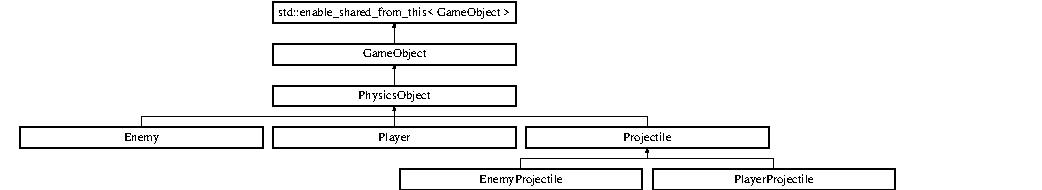
\includegraphics[height=2.527076cm]{d6/db5/class_physics_object}
\end{center}
\end{figure}
\subsection*{Public Member Functions}
\begin{DoxyCompactItemize}
\item 
\mbox{\Hypertarget{class_physics_object_a0dd37cc0f9535b676d3df937eaeb4780}\label{class_physics_object_a0dd37cc0f9535b676d3df937eaeb4780}} 
\hyperlink{class_physics_object_a0dd37cc0f9535b676d3df937eaeb4780}{Physics\+Object} ()
\begin{DoxyCompactList}\small\item\em Default Constructor. \end{DoxyCompactList}\item 
\hyperlink{class_physics_object_a8a92618716bd764c63f0ca80436a950c}{Physics\+Object} (const \hyperlink{class_game_object}{Game\+Object} \&game\+Object, const double \&object\+Size)
\begin{DoxyCompactList}\small\item\em Constructs the physics object based on the parameters provided. \end{DoxyCompactList}\item 
double \hyperlink{class_physics_object_adc592e9846ebedea3d58d50c5ada1c12}{get\+Size} () const
\begin{DoxyCompactList}\small\item\em gets the current size of the object \end{DoxyCompactList}\item 
virtual void \hyperlink{class_physics_object_a16163f4e5bf781b3814d024c9f44a276}{collision\+Action} (const Game\+Object\+Type \&object\+Type)
\begin{DoxyCompactList}\small\item\em Virtual function that is called whenever a collision occurs between this object and a different one. \end{DoxyCompactList}\end{DoxyCompactItemize}
\subsection*{Protected Attributes}
\begin{DoxyCompactItemize}
\item 
double \hyperlink{class_physics_object_a417a7eb051cfcfdbf8dfd0cc0875fa0d}{\+\_\+object\+Size}
\end{DoxyCompactItemize}
\subsection*{Additional Inherited Members}


\subsection{Detailed Description}
Acts as the main interface between the collision\+Detection and the game logic. 

Provides the size for the collision\+Detection to check as well as a function call for when a collision occurs. 

\subsection{Constructor \& Destructor Documentation}
\mbox{\Hypertarget{class_physics_object_a8a92618716bd764c63f0ca80436a950c}\label{class_physics_object_a8a92618716bd764c63f0ca80436a950c}} 
\index{Physics\+Object@{Physics\+Object}!Physics\+Object@{Physics\+Object}}
\index{Physics\+Object@{Physics\+Object}!Physics\+Object@{Physics\+Object}}
\subsubsection{\texorpdfstring{Physics\+Object()}{PhysicsObject()}}
{\footnotesize\ttfamily Physics\+Object\+::\+Physics\+Object (\begin{DoxyParamCaption}\item[{const \hyperlink{class_game_object}{Game\+Object} \&}]{game\+Object,  }\item[{const double \&}]{object\+Size }\end{DoxyParamCaption})}



Constructs the physics object based on the parameters provided. 


\begin{DoxyParams}{Parameters}
{\em game\+Object} & A copy of the gameobject is made and is applied to the object \\
\hline
{\em object\+Size} & The radial size of the object and its area of collision \\
\hline
\end{DoxyParams}


\subsection{Member Function Documentation}
\mbox{\Hypertarget{class_physics_object_a16163f4e5bf781b3814d024c9f44a276}\label{class_physics_object_a16163f4e5bf781b3814d024c9f44a276}} 
\index{Physics\+Object@{Physics\+Object}!collision\+Action@{collision\+Action}}
\index{collision\+Action@{collision\+Action}!Physics\+Object@{Physics\+Object}}
\subsubsection{\texorpdfstring{collision\+Action()}{collisionAction()}}
{\footnotesize\ttfamily void Physics\+Object\+::collision\+Action (\begin{DoxyParamCaption}\item[{const Game\+Object\+Type \&}]{object\+Type }\end{DoxyParamCaption})\hspace{0.3cm}{\ttfamily [virtual]}}



Virtual function that is called whenever a collision occurs between this object and a different one. 


\begin{DoxyParams}{Parameters}
{\em object\+Type} & The Game\+Object\+Type of the object that was collided with \\
\hline
\end{DoxyParams}


Reimplemented in \hyperlink{class_enemy_ac59660a58fac8d0ffdcb97c0717fa089}{Enemy}, \hyperlink{class_player_a1089079d7149a7fce6226935a6ce2f9c}{Player}, \hyperlink{class_player_projectile_a22fcdd7296d95b97ae60b4d20d8a57bd}{Player\+Projectile}, and \hyperlink{class_enemy_projectile_a4b3233a5ba7a3df66070cd6cdaa0362a}{Enemy\+Projectile}.

\mbox{\Hypertarget{class_physics_object_adc592e9846ebedea3d58d50c5ada1c12}\label{class_physics_object_adc592e9846ebedea3d58d50c5ada1c12}} 
\index{Physics\+Object@{Physics\+Object}!get\+Size@{get\+Size}}
\index{get\+Size@{get\+Size}!Physics\+Object@{Physics\+Object}}
\subsubsection{\texorpdfstring{get\+Size()}{getSize()}}
{\footnotesize\ttfamily double Physics\+Object\+::get\+Size (\begin{DoxyParamCaption}{ }\end{DoxyParamCaption}) const}



gets the current size of the object 

\begin{DoxyReturn}{Returns}
Returns the object size 
\end{DoxyReturn}


\subsection{Member Data Documentation}
\mbox{\Hypertarget{class_physics_object_a417a7eb051cfcfdbf8dfd0cc0875fa0d}\label{class_physics_object_a417a7eb051cfcfdbf8dfd0cc0875fa0d}} 
\index{Physics\+Object@{Physics\+Object}!\+\_\+object\+Size@{\+\_\+object\+Size}}
\index{\+\_\+object\+Size@{\+\_\+object\+Size}!Physics\+Object@{Physics\+Object}}
\subsubsection{\texorpdfstring{\+\_\+object\+Size}{\_objectSize}}
{\footnotesize\ttfamily double Physics\+Object\+::\+\_\+object\+Size\hspace{0.3cm}{\ttfamily [protected]}}

The radial collision size of the object 

The documentation for this class was generated from the following files\+:\begin{DoxyCompactItemize}
\item 
C\+:/\+Users/\+Tim/\+Documents/\+Software\+Dev/\+Software\+Project/\+Project\+Files/game-\/source-\/code/\+Front\+End\+Systems/Physics\+Object.\+h\item 
C\+:/\+Users/\+Tim/\+Documents/\+Software\+Dev/\+Software\+Project/\+Project\+Files/game-\/source-\/code/\+Front\+End\+Systems/Physics\+Object.\+cpp\end{DoxyCompactItemize}

\hypertarget{class_player}{}\section{Player Class Reference}
\label{class_player}\index{Player@{Player}}


\hyperlink{class_character}{Character} rework required here as well.  




{\ttfamily \#include $<$Player.\+h$>$}

Inheritance diagram for Player\+:\begin{figure}[H]
\begin{center}
\leavevmode
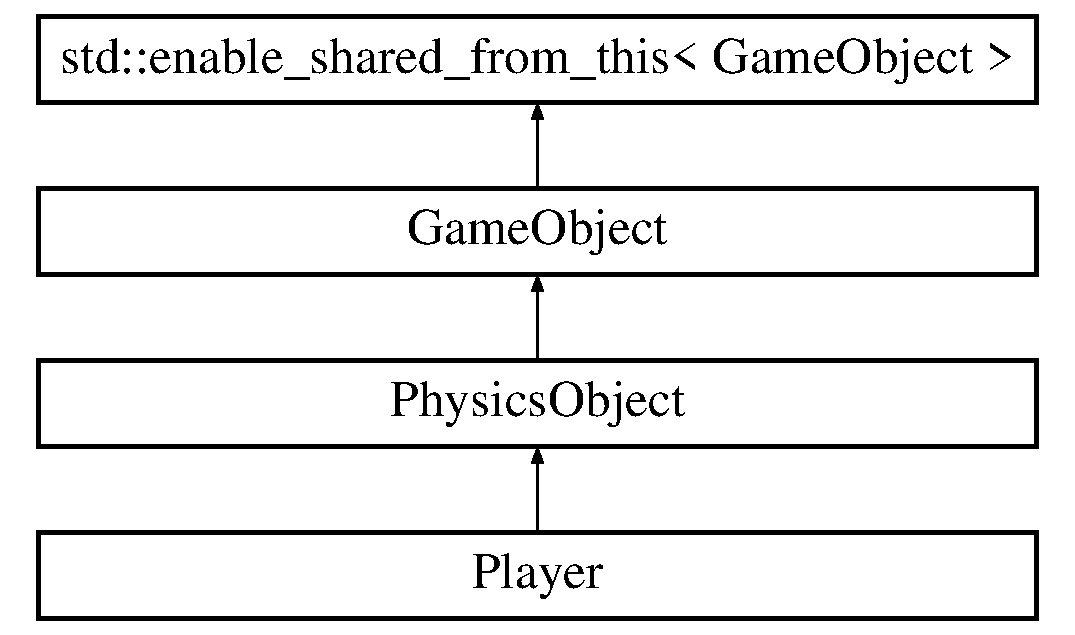
\includegraphics[height=4.000000cm]{d8/d53/class_player}
\end{center}
\end{figure}
\subsection*{Public Member Functions}
\begin{DoxyCompactItemize}
\item 
\mbox{\Hypertarget{class_player_affe0cc3cb714f6deb4e62f0c0d3f1fd8}\label{class_player_affe0cc3cb714f6deb4e62f0c0d3f1fd8}} 
\hyperlink{class_player_affe0cc3cb714f6deb4e62f0c0d3f1fd8}{Player} ()
\begin{DoxyCompactList}\small\item\em Redundant constructors need to be reworked. \end{DoxyCompactList}\item 
\hyperlink{class_player_afb985ed4c767e1ad824655b9f5f9d597}{Player} (\hyperlink{class_vector2_d}{Vector2D}$<$ double $>$ \&start\+Position, \hyperlink{class_character}{Character} player\+Stats)
\begin{DoxyCompactList}\small\item\em \hyperlink{class_player}{Player} constructor needs to be reworked too much database implementation is used. \end{DoxyCompactList}\item 
\mbox{\Hypertarget{class_player_a066cb6500937804121fd4ceb15595b3f}\label{class_player_a066cb6500937804121fd4ceb15595b3f}} 
{\bfseries Player} (\hyperlink{class_vector2_d}{Vector2D}$<$ double $>$ \&start\+Position, \hyperlink{class_character}{Character} player\+Stats, std\+::shared\+\_\+ptr$<$ \hyperlink{class_graphic_object}{Graphic\+Object} $>$ bullet\+Graphic)
\item 
\mbox{\Hypertarget{class_player_ad5023c3701c11222e09906b41c604135}\label{class_player_ad5023c3701c11222e09906b41c604135}} 
virtual \hyperlink{class_player}{Player} $\ast$ \hyperlink{class_player_ad5023c3701c11222e09906b41c604135}{Clone} () override
\begin{DoxyCompactList}\small\item\em Clone still in development. \end{DoxyCompactList}\item 
\mbox{\Hypertarget{class_player_a5e17be3418fa0ac0192c05efaf3dc8bd}\label{class_player_a5e17be3418fa0ac0192c05efaf3dc8bd}} 
void \hyperlink{class_player_a5e17be3418fa0ac0192c05efaf3dc8bd}{Update} () override
\begin{DoxyCompactList}\small\item\em could aslo be used as a friendship with scene \end{DoxyCompactList}\item 
virtual void \hyperlink{class_player_a965e7e8baf9b270e1b22784b890bc74d}{collision\+Action} (Game\+Object\+Type object\+Type) override
\item 
\mbox{\Hypertarget{class_player_a0bee9292374b568f74c2f9240fba0d36}\label{class_player_a0bee9292374b568f74c2f9240fba0d36}} 
const std\+::shared\+\_\+ptr$<$ \hyperlink{class_graphic_object}{Graphic\+Object} $>$ {\bfseries get\+Graphic\+Object} () override
\end{DoxyCompactItemize}
\subsection*{Additional Inherited Members}


\subsection{Detailed Description}
\hyperlink{class_character}{Character} rework required here as well. 

\subsection{Constructor \& Destructor Documentation}
\mbox{\Hypertarget{class_player_afb985ed4c767e1ad824655b9f5f9d597}\label{class_player_afb985ed4c767e1ad824655b9f5f9d597}} 
\index{Player@{Player}!Player@{Player}}
\index{Player@{Player}!Player@{Player}}
\subsubsection{\texorpdfstring{Player()}{Player()}}
{\footnotesize\ttfamily Player\+::\+Player (\begin{DoxyParamCaption}\item[{\hyperlink{class_vector2_d}{Vector2D}$<$ double $>$ \&}]{start\+Position,  }\item[{\hyperlink{class_character}{Character}}]{player\+Stats }\end{DoxyParamCaption})}



\hyperlink{class_player}{Player} constructor needs to be reworked too much database implementation is used. 

Needs to be stored in a database 

\subsection{Member Function Documentation}
\mbox{\Hypertarget{class_player_a965e7e8baf9b270e1b22784b890bc74d}\label{class_player_a965e7e8baf9b270e1b22784b890bc74d}} 
\index{Player@{Player}!collision\+Action@{collision\+Action}}
\index{collision\+Action@{collision\+Action}!Player@{Player}}
\subsubsection{\texorpdfstring{collision\+Action()}{collisionAction()}}
{\footnotesize\ttfamily void Player\+::collision\+Action (\begin{DoxyParamCaption}\item[{Game\+Object\+Type}]{object\+Type }\end{DoxyParamCaption})\hspace{0.3cm}{\ttfamily [override]}, {\ttfamily [virtual]}}

Magic Number needs to be removed (can be replaced by an enumerator class or static variable) 

Implements \hyperlink{class_physics_object}{Physics\+Object}.



The documentation for this class was generated from the following files\+:\begin{DoxyCompactItemize}
\item 
D\+:/\+Users/\+Tim-\/\+P\+C/\+Documents/\+Software\+\_\+\+I\+I/\+Project/\+Project\+Files/game-\/source-\/code/\+Front\+End\+Systems/Player.\+h\item 
D\+:/\+Users/\+Tim-\/\+P\+C/\+Documents/\+Software\+\_\+\+I\+I/\+Project/\+Project\+Files/game-\/source-\/code/\+Front\+End\+Systems/Player.\+cpp\end{DoxyCompactItemize}

\hypertarget{class_projectile}{}\section{Projectile Class Reference}
\label{class_projectile}\index{Projectile@{Projectile}}


{\ttfamily \#include $<$Projectile.\+h$>$}

Inheritance diagram for Projectile\+:\begin{figure}[H]
\begin{center}
\leavevmode
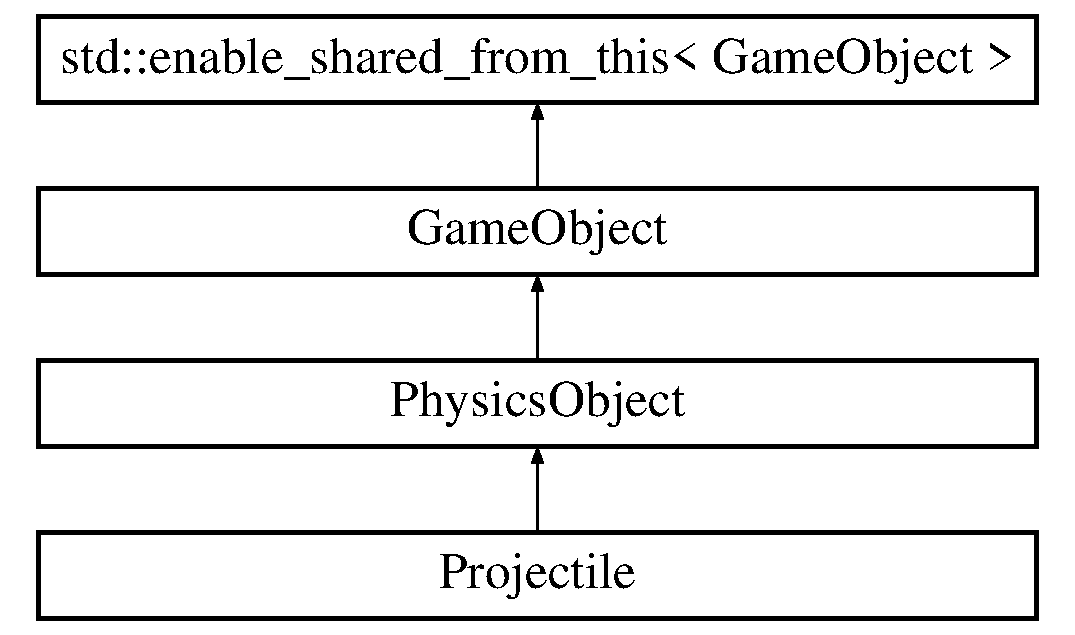
\includegraphics[height=4.000000cm]{db/dbe/class_projectile}
\end{center}
\end{figure}
\subsection*{Public Member Functions}
\begin{DoxyCompactItemize}
\item 
\mbox{\Hypertarget{class_projectile_ac536ed2aad56af866a2078b9a85aa16d}\label{class_projectile_ac536ed2aad56af866a2078b9a85aa16d}} 
\hyperlink{class_projectile_ac536ed2aad56af866a2078b9a85aa16d}{Projectile} ()
\begin{DoxyCompactList}\small\item\em Constructors need to be redesigned. \end{DoxyCompactList}\item 
\mbox{\Hypertarget{class_projectile_a45f5e2eb6db9f673670e9de0aa9b9bab}\label{class_projectile_a45f5e2eb6db9f673670e9de0aa9b9bab}} 
{\bfseries Projectile} (Game\+Object\+Type projectile\+Type)
\item 
\mbox{\Hypertarget{class_projectile_a6d13e20ed5be714a7efd4be89791ea94}\label{class_projectile_a6d13e20ed5be714a7efd4be89791ea94}} 
\hyperlink{class_projectile_a6d13e20ed5be714a7efd4be89791ea94}{Projectile} (std\+::shared\+\_\+ptr$<$ \hyperlink{class_graphic_object}{Graphic\+Object} $>$ bullet\+Graphic, Game\+Object\+Type projectile\+Type, \hyperlink{structxy_vector}{xy\+Vector} scale)
\begin{DoxyCompactList}\small\item\em Constructor Needs a Database Dependency. \end{DoxyCompactList}\item 
\mbox{\Hypertarget{class_projectile_a60b9863678645f9605bf938ef6df7938}\label{class_projectile_a60b9863678645f9605bf938ef6df7938}} 
{\bfseries Projectile} (const \hyperlink{class_projectile}{Projectile} \&copy\+Projectile)
\item 
\mbox{\Hypertarget{class_projectile_ad057a8aeadb0064aacd0f93b2d6de158}\label{class_projectile_ad057a8aeadb0064aacd0f93b2d6de158}} 
virtual void \hyperlink{class_projectile_ad057a8aeadb0064aacd0f93b2d6de158}{Update} () override
\begin{DoxyCompactList}\small\item\em could aslo be used as a friendship with scene \end{DoxyCompactList}\item 
\mbox{\Hypertarget{class_projectile_aedb2c1ee7933578088e4d2a60d9c0f5c}\label{class_projectile_aedb2c1ee7933578088e4d2a60d9c0f5c}} 
void {\bfseries Initialise} (\hyperlink{class_vector2_d}{Vector2D}$<$ double $>$ starting\+Pos, \hyperlink{class_vector2_d}{Vector2D}$<$ double $>$ direction, double move\+Speed)
\item 
\mbox{\Hypertarget{class_projectile_a8dae5b6cc0293fc6c85797fcf2019492}\label{class_projectile_a8dae5b6cc0293fc6c85797fcf2019492}} 
virtual void \hyperlink{class_projectile_a8dae5b6cc0293fc6c85797fcf2019492}{collision\+Action} (Game\+Object\+Type object\+Type) override
\begin{DoxyCompactList}\small\item\em polymorphism will reduce this complexity \end{DoxyCompactList}\item 
\mbox{\Hypertarget{class_projectile_a639f52184c8b9720ca8c36371303332d}\label{class_projectile_a639f52184c8b9720ca8c36371303332d}} 
virtual const std\+::shared\+\_\+ptr$<$ \hyperlink{class_graphic_object}{Graphic\+Object} $>$ {\bfseries get\+Graphic\+Object} () override
\item 
\mbox{\Hypertarget{class_projectile_a39653a4aa80df0364e15854f0f5e389d}\label{class_projectile_a39653a4aa80df0364e15854f0f5e389d}} 
virtual \hyperlink{class_projectile}{Projectile} $\ast$ \hyperlink{class_projectile_a39653a4aa80df0364e15854f0f5e389d}{Clone} () override
\begin{DoxyCompactList}\small\item\em Clone Function Still in development. \end{DoxyCompactList}\item 
\mbox{\Hypertarget{class_projectile_add4d983566a326200ea1d7c74737e108}\label{class_projectile_add4d983566a326200ea1d7c74737e108}} 
\hyperlink{class_projectile_add4d983566a326200ea1d7c74737e108}{$\sim$\+Projectile} () override
\begin{DoxyCompactList}\small\item\em Needs the virtual tag. \end{DoxyCompactList}\end{DoxyCompactItemize}
\subsection*{Additional Inherited Members}


\subsection{Detailed Description}
Object needs to be converted into a polymorphic object, one for player and one for enemy with virtual destorys and boundaries corresponds to the type information in a better way 

The documentation for this class was generated from the following files\+:\begin{DoxyCompactItemize}
\item 
D\+:/\+Users/\+Tim-\/\+P\+C/\+Documents/\+Software\+\_\+\+I\+I/\+Project/\+Project\+Files/game-\/source-\/code/\+Front\+End\+Systems/Projectile.\+h\item 
D\+:/\+Users/\+Tim-\/\+P\+C/\+Documents/\+Software\+\_\+\+I\+I/\+Project/\+Project\+Files/game-\/source-\/code/\+Front\+End\+Systems/Projectile.\+cpp\end{DoxyCompactItemize}

\hypertarget{class_scene}{}\section{Scene Class Reference}
\label{class_scene}\index{Scene@{Scene}}
Inheritance diagram for Scene\+:\begin{figure}[H]
\begin{center}
\leavevmode
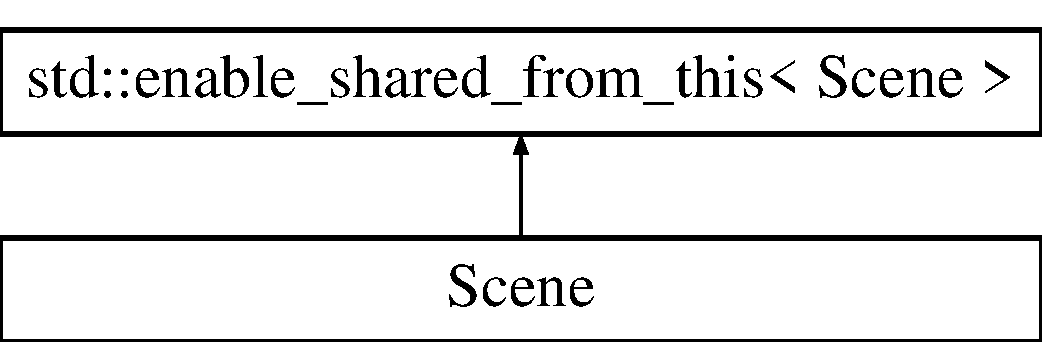
\includegraphics[height=2.000000cm]{d6/db5/class_scene}
\end{center}
\end{figure}
\subsection*{Public Member Functions}
\begin{DoxyCompactItemize}
\item 
\mbox{\Hypertarget{class_scene_a0caa1ccf717fe21059f20b0c4a57cde6}\label{class_scene_a0caa1ccf717fe21059f20b0c4a57cde6}} 
\hyperlink{class_scene_a0caa1ccf717fe21059f20b0c4a57cde6}{Scene} (const \hyperlink{class_scene}{Scene} \&rhs)
\begin{DoxyCompactList}\small\item\em Currently needs to be fixed. \end{DoxyCompactList}\item 
\mbox{\Hypertarget{class_scene_a1d902efeacc113ceb2dd79a976b04a77}\label{class_scene_a1d902efeacc113ceb2dd79a976b04a77}} 
void {\bfseries Scene\+Update} ()
\item 
void \hyperlink{class_scene_a3dd730cba4a22bf75e54c4b644c26976}{Instantiate} (shared\+\_\+ptr$<$ \hyperlink{class_game_object}{Game\+Object} $>$ game\+Obj)
\item 
\mbox{\Hypertarget{class_scene_ae418f788bfbf2551d89e907d1d4cf2f6}\label{class_scene_ae418f788bfbf2551d89e907d1d4cf2f6}} 
void {\bfseries Destroy\+Game\+Object} (game\+Obj\+\_\+ptr game\+Object)
\item 
\mbox{\Hypertarget{class_scene_a0696711d2b1452f3d6f42f7a92f4218d}\label{class_scene_a0696711d2b1452f3d6f42f7a92f4218d}} 
std\+::vector$<$ game\+Obj\+\_\+ptr $>$ {\bfseries get\+Game\+Object\+List} () const
\item 
\mbox{\Hypertarget{class_scene_a64a47e6503f634ea2b76fa2078538716}\label{class_scene_a64a47e6503f634ea2b76fa2078538716}} 
\hyperlink{class_scene}{Scene} \& {\bfseries operator=} (const \hyperlink{class_scene}{Scene} \&rhs)
\end{DoxyCompactItemize}
\subsection*{Public Attributes}
\begin{DoxyCompactItemize}
\item 
\mbox{\Hypertarget{class_scene_a29183cf37f5227ea9a82d2a15c42336c}\label{class_scene_a29183cf37f5227ea9a82d2a15c42336c}} 
std\+::mutex {\bfseries \+\_\+game\+Object\+\_\+list\+\_\+mutex}
\end{DoxyCompactItemize}
\subsection*{Private Attributes}
\begin{DoxyCompactItemize}
\item 
std\+::vector$<$ game\+Obj\+\_\+ptr $>$ \hyperlink{class_scene_af1956432917d14b0a0b26103dbcb5bcd}{\+\_\+game\+Object\+\_\+list}
\end{DoxyCompactItemize}


\subsection{Member Function Documentation}
\mbox{\Hypertarget{class_scene_a3dd730cba4a22bf75e54c4b644c26976}\label{class_scene_a3dd730cba4a22bf75e54c4b644c26976}} 
\index{Scene@{Scene}!Instantiate@{Instantiate}}
\index{Instantiate@{Instantiate}!Scene@{Scene}}
\subsubsection{\texorpdfstring{Instantiate()}{Instantiate()}}
{\footnotesize\ttfamily void Scene\+::\+Instantiate (\begin{DoxyParamCaption}\item[{shared\+\_\+ptr$<$ \hyperlink{class_game_object}{Game\+Object} $>$}]{game\+Obj }\end{DoxyParamCaption})}

Seems redundant to do duplicate the game object pointer 

\subsection{Member Data Documentation}
\mbox{\Hypertarget{class_scene_af1956432917d14b0a0b26103dbcb5bcd}\label{class_scene_af1956432917d14b0a0b26103dbcb5bcd}} 
\index{Scene@{Scene}!\+\_\+game\+Object\+\_\+list@{\+\_\+game\+Object\+\_\+list}}
\index{\+\_\+game\+Object\+\_\+list@{\+\_\+game\+Object\+\_\+list}!Scene@{Scene}}
\subsubsection{\texorpdfstring{\+\_\+game\+Object\+\_\+list}{\_gameObject\_list}}
{\footnotesize\ttfamily std\+::vector$<$game\+Obj\+\_\+ptr$>$ Scene\+::\+\_\+game\+Object\+\_\+list\hspace{0.3cm}{\ttfamily [private]}}

would be better to use a doubly linked list instead of a vector since it has a better time effeciency when it deals with insertion and deletion of elements 

The documentation for this class was generated from the following files\+:\begin{DoxyCompactItemize}
\item 
D\+:/\+Users/\+Tim-\/\+P\+C/\+Documents/\+Software\+\_\+\+I\+I/\+Project/\+Project\+Files/game-\/source-\/code/\+Front\+End\+Systems/Scene.\+h\item 
D\+:/\+Users/\+Tim-\/\+P\+C/\+Documents/\+Software\+\_\+\+I\+I/\+Project/\+Project\+Files/game-\/source-\/code/\+Front\+End\+Systems/Scene.\+cpp\end{DoxyCompactItemize}

\hypertarget{class_scene_doesnt_exist}{}\section{Scene\+Doesnt\+Exist Class Reference}
\label{class_scene_doesnt_exist}\index{Scene\+Doesnt\+Exist@{Scene\+Doesnt\+Exist}}


Exception thrown if a scene does not exist at the specific index that is requested.  




{\ttfamily \#include $<$Game\+Manager.\+h$>$}



\subsection{Detailed Description}
Exception thrown if a scene does not exist at the specific index that is requested. 

The documentation for this class was generated from the following file\+:\begin{DoxyCompactItemize}
\item 
D\+:/\+Users/\+Tim-\/\+P\+C/\+Documents/\+Software\+\_\+\+I\+I/\+Project/\+Project\+Files/game-\/source-\/code/\+Back\+End\+Systems/Game\+Manager.\+h\end{DoxyCompactItemize}

\hypertarget{class_shoot_component}{}\section{Shoot\+Component Class Reference}
\label{class_shoot_component}\index{Shoot\+Component@{Shoot\+Component}}
\subsection*{Public Member Functions}
\begin{DoxyCompactItemize}
\item 
\mbox{\Hypertarget{class_shoot_component_acfbe65399cebcc06d04eeb18807642f5}\label{class_shoot_component_acfbe65399cebcc06d04eeb18807642f5}} 
\hyperlink{class_shoot_component_acfbe65399cebcc06d04eeb18807642f5}{Shoot\+Component} ()
\begin{DoxyCompactList}\small\item\em redundant Constructors that do not conform to the class invariance \end{DoxyCompactList}\item 
\hyperlink{class_shoot_component_a3c0334d147d54522d58a379d6e473006}{Shoot\+Component} (const std\+::shared\+\_\+ptr$<$ \hyperlink{class_graphic_object}{Graphic\+Object} $>$ \&bullet\+Graphic, Game\+Object\+Type bullet\+Type)
\begin{DoxyCompactList}\small\item\em will be removed once the Template projectile is set up \end{DoxyCompactList}\item 
\hyperlink{class_shoot_component_a38ab688c7cf0775b4f15124a1c02bfc7}{Shoot\+Component} (std\+::shared\+\_\+ptr$<$ \hyperlink{class_projectile}{Projectile} $>$ bullet)
\begin{DoxyCompactList}\small\item\em correct constructor \end{DoxyCompactList}\item 
void \hyperlink{class_shoot_component_a27a553ba952e96c77bc6e7d2e5ca9f0a}{Shoot} (\hyperlink{class_vector2_d}{Vector2D}$<$ double $>$ target, \hyperlink{class_vector2_d}{Vector2D}$<$ double $>$ start\+Position, double shoot\+Speed, \hyperlink{class_scene}{Scene} \&scene)
\begin{DoxyCompactList}\small\item\em \hyperlink{class_scene}{Scene} needs to be moved into the constructor should be the current scene (use of Application Class) \end{DoxyCompactList}\end{DoxyCompactItemize}
\subsection*{Private Attributes}
\begin{DoxyCompactItemize}
\item 
\mbox{\Hypertarget{class_shoot_component_a1f7cba7f1948db5f6150d96163c64f52}\label{class_shoot_component_a1f7cba7f1948db5f6150d96163c64f52}} 
std\+::shared\+\_\+ptr$<$ \hyperlink{class_projectile}{Projectile} $>$ {\bfseries \+\_\+bullet}
\end{DoxyCompactItemize}


\subsection{Constructor \& Destructor Documentation}
\mbox{\Hypertarget{class_shoot_component_a3c0334d147d54522d58a379d6e473006}\label{class_shoot_component_a3c0334d147d54522d58a379d6e473006}} 
\index{Shoot\+Component@{Shoot\+Component}!Shoot\+Component@{Shoot\+Component}}
\index{Shoot\+Component@{Shoot\+Component}!Shoot\+Component@{Shoot\+Component}}
\subsubsection{\texorpdfstring{Shoot\+Component()}{ShootComponent()}\hspace{0.1cm}{\footnotesize\ttfamily [1/2]}}
{\footnotesize\ttfamily Shoot\+Component\+::\+Shoot\+Component (\begin{DoxyParamCaption}\item[{const std\+::shared\+\_\+ptr$<$ \hyperlink{class_graphic_object}{Graphic\+Object} $>$ \&}]{bullet\+Graphic,  }\item[{Game\+Object\+Type}]{bullet\+Type }\end{DoxyParamCaption})}



will be removed once the Template projectile is set up 

Constructor will need to be deleted. \mbox{\Hypertarget{class_shoot_component_a38ab688c7cf0775b4f15124a1c02bfc7}\label{class_shoot_component_a38ab688c7cf0775b4f15124a1c02bfc7}} 
\index{Shoot\+Component@{Shoot\+Component}!Shoot\+Component@{Shoot\+Component}}
\index{Shoot\+Component@{Shoot\+Component}!Shoot\+Component@{Shoot\+Component}}
\subsubsection{\texorpdfstring{Shoot\+Component()}{ShootComponent()}\hspace{0.1cm}{\footnotesize\ttfamily [2/2]}}
{\footnotesize\ttfamily Shoot\+Component\+::\+Shoot\+Component (\begin{DoxyParamCaption}\item[{std\+::shared\+\_\+ptr$<$ \hyperlink{class_projectile}{Projectile} $>$}]{bullet }\end{DoxyParamCaption})}



correct constructor 

correct type of constructor 

\subsection{Member Function Documentation}
\mbox{\Hypertarget{class_shoot_component_a27a553ba952e96c77bc6e7d2e5ca9f0a}\label{class_shoot_component_a27a553ba952e96c77bc6e7d2e5ca9f0a}} 
\index{Shoot\+Component@{Shoot\+Component}!Shoot@{Shoot}}
\index{Shoot@{Shoot}!Shoot\+Component@{Shoot\+Component}}
\subsubsection{\texorpdfstring{Shoot()}{Shoot()}}
{\footnotesize\ttfamily void Shoot\+Component\+::\+Shoot (\begin{DoxyParamCaption}\item[{\hyperlink{class_vector2_d}{Vector2D}$<$ double $>$}]{target,  }\item[{\hyperlink{class_vector2_d}{Vector2D}$<$ double $>$}]{start\+Position,  }\item[{double}]{shoot\+Speed,  }\item[{\hyperlink{class_scene}{Scene} \&}]{scene }\end{DoxyParamCaption})}



\hyperlink{class_scene}{Scene} needs to be moved into the constructor should be the current scene (use of Application Class) 

can be implemented in a better way with the vector functions 

The documentation for this class was generated from the following files\+:\begin{DoxyCompactItemize}
\item 
D\+:/\+Users/\+Tim-\/\+P\+C/\+Documents/\+Software\+\_\+\+I\+I/\+Project/\+Project\+Files/game-\/source-\/code/\+Front\+End\+Systems/Shoot\+Component.\+h\item 
D\+:/\+Users/\+Tim-\/\+P\+C/\+Documents/\+Software\+\_\+\+I\+I/\+Project/\+Project\+Files/game-\/source-\/code/\+Front\+End\+Systems/Shoot\+Component.\+cpp\end{DoxyCompactItemize}

\hypertarget{class_singleton_exists}{}\section{Singleton\+Exists Class Reference}
\label{class_singleton_exists}\index{Singleton\+Exists@{Singleton\+Exists}}


The documentation for this class was generated from the following file\+:\begin{DoxyCompactItemize}
\item 
D\+:/\+Users/\+Tim-\/\+P\+C/\+Documents/\+Software\+\_\+\+I\+I/\+Project/\+Project\+Files/game-\/source-\/code/\+Back\+End\+Systems/My\+Singleton.\+h\end{DoxyCompactItemize}

\hypertarget{class_splash_screen}{}\section{Splash\+Screen Class Reference}
\label{class_splash_screen}\index{Splash\+Screen@{Splash\+Screen}}


\hyperlink{class_splash_screen}{Splash\+Screen} is used to represent a background image within the game and has the responsibility of loading the game scene and exiting the game.  




{\ttfamily \#include $<$Splash\+Screen.\+h$>$}

Inheritance diagram for Splash\+Screen\+:\begin{figure}[H]
\begin{center}
\leavevmode
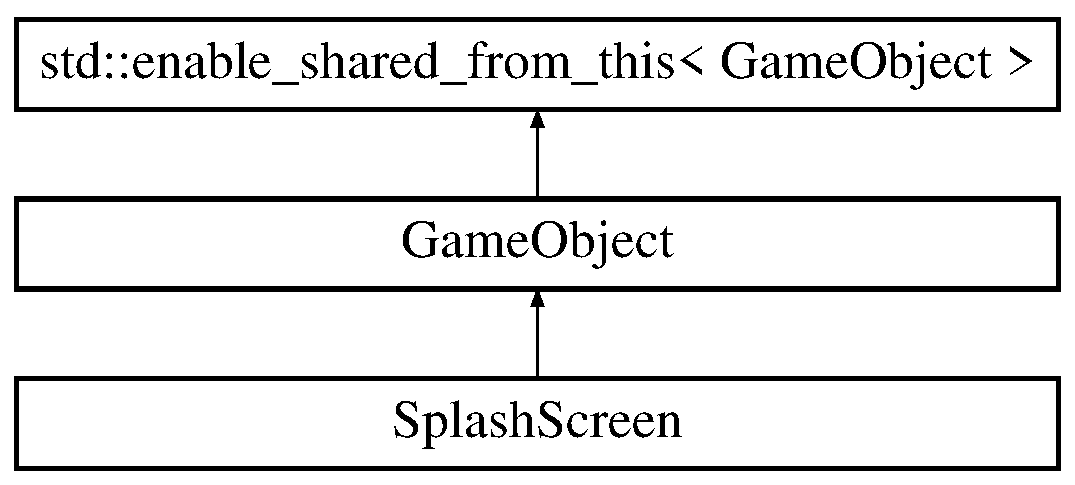
\includegraphics[height=3.000000cm]{da/d1c/class_splash_screen}
\end{center}
\end{figure}
\subsection*{Public Member Functions}
\begin{DoxyCompactItemize}
\item 
\hyperlink{class_splash_screen_afefa0db946b214828634c7f2550677e6}{Splash\+Screen} (const \hyperlink{class_game_object}{Game\+Object} \&game\+Object)
\begin{DoxyCompactList}\small\item\em The constructor for a splashscreen takes in a gameobject which is copied into the base gameobject of class to define the base parameters. \end{DoxyCompactList}\item 
\mbox{\Hypertarget{class_splash_screen_af78b8eab226a89fec389e53cbf3ed9e8}\label{class_splash_screen_af78b8eab226a89fec389e53cbf3ed9e8}} 
void \hyperlink{class_splash_screen_af78b8eab226a89fec389e53cbf3ed9e8}{Update} () override
\begin{DoxyCompactList}\small\item\em Checks for user input to identify if the Game \hyperlink{class_scene}{Scene} should be loaded/\+Restarted or if the game should exit. \end{DoxyCompactList}\end{DoxyCompactItemize}
\subsection*{Private Member Functions}
\begin{DoxyCompactItemize}
\item 
\mbox{\Hypertarget{class_splash_screen_a5d9ac6cec631b24cc947dda245e7d151}\label{class_splash_screen_a5d9ac6cec631b24cc947dda245e7d151}} 
void \hyperlink{class_splash_screen_a5d9ac6cec631b24cc947dda245e7d151}{Quit\+Game} ()
\begin{DoxyCompactList}\small\item\em Quits the game when escape is pressed. \end{DoxyCompactList}\item 
\mbox{\Hypertarget{class_splash_screen_a008328b85475bd01e326f94f20bf9217}\label{class_splash_screen_a008328b85475bd01e326f94f20bf9217}} 
void \hyperlink{class_splash_screen_a008328b85475bd01e326f94f20bf9217}{Play\+Game} ()
\begin{DoxyCompactList}\small\item\em Loads the game \hyperlink{class_scene}{Scene} when Enter is pressed. \end{DoxyCompactList}\end{DoxyCompactItemize}
\subsection*{Additional Inherited Members}


\subsection{Detailed Description}
\hyperlink{class_splash_screen}{Splash\+Screen} is used to represent a background image within the game and has the responsibility of loading the game scene and exiting the game. 

The class responsibilities of this class are should rather be seperated into a Background\+Object and a Menu\+Controller object it is currently designed incorrectly 

\subsection{Constructor \& Destructor Documentation}
\mbox{\Hypertarget{class_splash_screen_afefa0db946b214828634c7f2550677e6}\label{class_splash_screen_afefa0db946b214828634c7f2550677e6}} 
\index{Splash\+Screen@{Splash\+Screen}!Splash\+Screen@{Splash\+Screen}}
\index{Splash\+Screen@{Splash\+Screen}!Splash\+Screen@{Splash\+Screen}}
\subsubsection{\texorpdfstring{Splash\+Screen()}{SplashScreen()}}
{\footnotesize\ttfamily Splash\+Screen\+::\+Splash\+Screen (\begin{DoxyParamCaption}\item[{const \hyperlink{class_game_object}{Game\+Object} \&}]{game\+Object }\end{DoxyParamCaption})}



The constructor for a splashscreen takes in a gameobject which is copied into the base gameobject of class to define the base parameters. 


\begin{DoxyParams}{Parameters}
{\em game\+Object} & \hyperlink{class_game_object}{Game\+Object} that contains the base parameters for the current instance of the \hyperlink{class_splash_screen}{Splash\+Screen} \\
\hline
\end{DoxyParams}


The documentation for this class was generated from the following files\+:\begin{DoxyCompactItemize}
\item 
D\+:/\+Users/\+Tim-\/\+P\+C/\+Documents/\+Software\+\_\+\+I\+I/\+Project/\+Project\+Files/game-\/source-\/code/\+Front\+End\+Systems/Splash\+Screen.\+h\item 
D\+:/\+Users/\+Tim-\/\+P\+C/\+Documents/\+Software\+\_\+\+I\+I/\+Project/\+Project\+Files/game-\/source-\/code/\+Front\+End\+Systems/Splash\+Screen.\+cpp\end{DoxyCompactItemize}

\hypertarget{struct_sprite_info}{}\section{Sprite\+Info Struct Reference}
\label{struct_sprite_info}\index{Sprite\+Info@{Sprite\+Info}}


{\ttfamily \#include $<$Sprite\+Info.\+h$>$}

\subsection*{Public Attributes}
\begin{DoxyCompactItemize}
\item 
\mbox{\Hypertarget{struct_sprite_info_a0cbb7ab027f95f8b936eaaa021d51ce9}\label{struct_sprite_info_a0cbb7ab027f95f8b936eaaa021d51ce9}} 
Sprite {\bfseries sprite}
\item 
\mbox{\Hypertarget{struct_sprite_info_a29a5ebd0f1e39394af99bee4658b2b8a}\label{struct_sprite_info_a29a5ebd0f1e39394af99bee4658b2b8a}} 
Texture {\bfseries texture}
\end{DoxyCompactItemize}


\subsection{Detailed Description}
Neeeds complete Restructuring \hyperlink{struct_sprite_info}{Sprite\+Info} should be form part of the \hyperlink{class_display_manager}{Display\+Manager} and Sprite\+Data should be part of the Gameobject 

The documentation for this struct was generated from the following file\+:\begin{DoxyCompactItemize}
\item 
D\+:/\+Users/\+Tim-\/\+P\+C/\+Documents/\+Software\+\_\+\+I\+I/\+Project/\+Project\+Files/game-\/source-\/code/\+Front\+End\+Systems/Sprite\+Info.\+h\end{DoxyCompactItemize}

\hypertarget{class_update_game_object_display}{}\section{Update\+Game\+Object\+Display Class Reference}
\label{class_update_game_object_display}\index{Update\+Game\+Object\+Display@{Update\+Game\+Object\+Display}}


Updates the Sprite position and scale for each Game\+Oject.  




{\ttfamily \#include $<$Update\+Game\+Object\+Display.\+h$>$}

\subsection*{Public Member Functions}
\begin{DoxyCompactItemize}
\item 
const sf\+::\+Sprite \& \hyperlink{class_update_game_object_display_ac17a26f7563060fb9d4a0eb8959b1d29}{Determine\+Game\+Object\+Changes} (shared\+\_\+ptr$<$ \hyperlink{class_game_object}{Game\+Object} $>$ GO)
\begin{DoxyCompactList}\small\item\em Identifies and applies any changes made to a \hyperlink{class_game_object}{Game\+Object} and updates a sprite that corresponds to the changes in scale and position of that \hyperlink{class_game_object}{Game\+Object}. \end{DoxyCompactList}\item 
const unsigned int \hyperlink{class_update_game_object_display_a84972d99bd8f15ca869fc3710b836283}{get\+Hash\+Table\+Size} () const
\begin{DoxyCompactList}\small\item\em determines the current size of the hashtable made up of \hyperlink{struct_sprite_info}{Sprite\+Info} \end{DoxyCompactList}\end{DoxyCompactItemize}
\subsection*{Private Member Functions}
\begin{DoxyCompactItemize}
\item 
void \hyperlink{class_update_game_object_display_ab9405bbbabaa083cfdaefbbe84cb7cd4}{Initialise\+Sprite\+Info} (const \hyperlink{class_graphic_object}{Graphic\+Object} \&graphic\+Object)
\begin{DoxyCompactList}\small\item\em Initialises the Sprite Info that corresponds with the graphic object that is being drawn. Is only called when a \hyperlink{struct_sprite_info}{Sprite\+Info} does not exist inside of the hash table. \end{DoxyCompactList}\item 
const sf\+::\+Sprite \& \hyperlink{class_update_game_object_display_a05f0b24dfb3e2206b0d363dbc5127139}{Update\+Sprite\+Properties} (const \hyperlink{class_vector2_d}{Vector2D} \&position, const \hyperlink{structxy_vector}{xy\+Vector} \&scale, const string \&current\+Object\+Key)
\begin{DoxyCompactList}\small\item\em Updates the sprite properties according to the information from the corresponding \hyperlink{class_game_object}{Game\+Object}. \end{DoxyCompactList}\item 
bool \hyperlink{class_update_game_object_display_a10502ed4d422e5bab6b5f3591d392c55}{Check\+If\+Sprite\+Info\+Exists} (const \hyperlink{class_graphic_object}{Graphic\+Object} \&corresponding\+Graphic)
\begin{DoxyCompactList}\small\item\em Checks if the \hyperlink{struct_sprite_info}{Sprite\+Info} that corresponds to a particular graphic object has already been generated and is being stored in the hash table. \end{DoxyCompactList}\end{DoxyCompactItemize}
\subsection*{Private Attributes}
\begin{DoxyCompactItemize}
\item 
std\+::unordered\+\_\+map$<$ std\+::string, std\+::shared\+\_\+ptr$<$ \hyperlink{struct_sprite_info}{Sprite\+Info} $>$ $>$ \hyperlink{class_update_game_object_display_a51ae3f07958294b737885c9a0bd86153}{\+\_\+sprite\+Info\+Table}
\end{DoxyCompactItemize}


\subsection{Detailed Description}
Updates the Sprite position and scale for each Game\+Oject. 

contains a hash table that stores the individual sprites and corresponding textures for the specific key provided within the \hyperlink{class_graphic_object}{Graphic\+Object} composition of the \hyperlink{class_game_object}{Game\+Object}. Updates the screen position and scale of the sprite for each game object provided. If the sprite and texture do not exist inside of the hash table it is created and added into it. 

\subsection{Member Function Documentation}
\mbox{\Hypertarget{class_update_game_object_display_a10502ed4d422e5bab6b5f3591d392c55}\label{class_update_game_object_display_a10502ed4d422e5bab6b5f3591d392c55}} 
\index{Update\+Game\+Object\+Display@{Update\+Game\+Object\+Display}!Check\+If\+Sprite\+Info\+Exists@{Check\+If\+Sprite\+Info\+Exists}}
\index{Check\+If\+Sprite\+Info\+Exists@{Check\+If\+Sprite\+Info\+Exists}!Update\+Game\+Object\+Display@{Update\+Game\+Object\+Display}}
\subsubsection{\texorpdfstring{Check\+If\+Sprite\+Info\+Exists()}{CheckIfSpriteInfoExists()}}
{\footnotesize\ttfamily bool Update\+Game\+Object\+Display\+::\+Check\+If\+Sprite\+Info\+Exists (\begin{DoxyParamCaption}\item[{const \hyperlink{class_graphic_object}{Graphic\+Object} \&}]{corresponding\+Graphic }\end{DoxyParamCaption})\hspace{0.3cm}{\ttfamily [private]}}



Checks if the \hyperlink{struct_sprite_info}{Sprite\+Info} that corresponds to a particular graphic object has already been generated and is being stored in the hash table. 


\begin{DoxyParams}{Parameters}
{\em corresponding\+Graphic} & The Corresponding \hyperlink{class_graphic_object}{Graphic\+Object} to the \hyperlink{struct_sprite_info}{Sprite\+Info} in the table \\
\hline
\end{DoxyParams}
\begin{DoxyReturn}{Returns}
returns true if the \hyperlink{struct_sprite_info}{Sprite\+Info} does Exist
\end{DoxyReturn}
Determines whether the \hyperlink{struct_sprite_info}{Sprite\+Info} object that corresponds to the key obtained from the graphic object exists. Uses std\+::find to check for the object and returns a true if the iterator returned is not equal to the end of the hash table \mbox{\Hypertarget{class_update_game_object_display_ac17a26f7563060fb9d4a0eb8959b1d29}\label{class_update_game_object_display_ac17a26f7563060fb9d4a0eb8959b1d29}} 
\index{Update\+Game\+Object\+Display@{Update\+Game\+Object\+Display}!Determine\+Game\+Object\+Changes@{Determine\+Game\+Object\+Changes}}
\index{Determine\+Game\+Object\+Changes@{Determine\+Game\+Object\+Changes}!Update\+Game\+Object\+Display@{Update\+Game\+Object\+Display}}
\subsubsection{\texorpdfstring{Determine\+Game\+Object\+Changes()}{DetermineGameObjectChanges()}}
{\footnotesize\ttfamily const sf\+::\+Sprite \& Update\+Game\+Object\+Display\+::\+Determine\+Game\+Object\+Changes (\begin{DoxyParamCaption}\item[{shared\+\_\+ptr$<$ \hyperlink{class_game_object}{Game\+Object} $>$}]{GO }\end{DoxyParamCaption})}



Identifies and applies any changes made to a \hyperlink{class_game_object}{Game\+Object} and updates a sprite that corresponds to the changes in scale and position of that \hyperlink{class_game_object}{Game\+Object}. 


\begin{DoxyParams}{Parameters}
{\em GO} & an std\+::shared\+\_\+ptr to the \hyperlink{class_game_object}{Game\+Object} that is being checked for changes\\
\hline
\end{DoxyParams}
Initially Identifies if the \hyperlink{class_game_object}{Game\+Object}\textquotesingle{}s corresponding sprite has been drawn before. If it does not exist a texture is created according to the information stored inside of the \hyperlink{class_graphic_object}{Graphic\+Object} Composition and the sprite is setup accordingly. After which the sprite is updated to the corresponding scale and position of the \hyperlink{class_game_object}{Game\+Object} \mbox{\Hypertarget{class_update_game_object_display_a84972d99bd8f15ca869fc3710b836283}\label{class_update_game_object_display_a84972d99bd8f15ca869fc3710b836283}} 
\index{Update\+Game\+Object\+Display@{Update\+Game\+Object\+Display}!get\+Hash\+Table\+Size@{get\+Hash\+Table\+Size}}
\index{get\+Hash\+Table\+Size@{get\+Hash\+Table\+Size}!Update\+Game\+Object\+Display@{Update\+Game\+Object\+Display}}
\subsubsection{\texorpdfstring{get\+Hash\+Table\+Size()}{getHashTableSize()}}
{\footnotesize\ttfamily const unsigned int Update\+Game\+Object\+Display\+::get\+Hash\+Table\+Size (\begin{DoxyParamCaption}{ }\end{DoxyParamCaption}) const\hspace{0.3cm}{\ttfamily [inline]}}



determines the current size of the hashtable made up of \hyperlink{struct_sprite_info}{Sprite\+Info} 

\begin{DoxyReturn}{Returns}
Returns the size of the hashtable used to store the various \hyperlink{struct_sprite_info}{Sprite\+Info} Objects 
\end{DoxyReturn}
\mbox{\Hypertarget{class_update_game_object_display_ab9405bbbabaa083cfdaefbbe84cb7cd4}\label{class_update_game_object_display_ab9405bbbabaa083cfdaefbbe84cb7cd4}} 
\index{Update\+Game\+Object\+Display@{Update\+Game\+Object\+Display}!Initialise\+Sprite\+Info@{Initialise\+Sprite\+Info}}
\index{Initialise\+Sprite\+Info@{Initialise\+Sprite\+Info}!Update\+Game\+Object\+Display@{Update\+Game\+Object\+Display}}
\subsubsection{\texorpdfstring{Initialise\+Sprite\+Info()}{InitialiseSpriteInfo()}}
{\footnotesize\ttfamily void Update\+Game\+Object\+Display\+::\+Initialise\+Sprite\+Info (\begin{DoxyParamCaption}\item[{const \hyperlink{class_graphic_object}{Graphic\+Object} \&}]{graphic\+Object }\end{DoxyParamCaption})\hspace{0.3cm}{\ttfamily [private]}}



Initialises the Sprite Info that corresponds with the graphic object that is being drawn. Is only called when a \hyperlink{struct_sprite_info}{Sprite\+Info} does not exist inside of the hash table. 


\begin{DoxyParams}{Parameters}
{\em graphic\+Object} & The \hyperlink{class_graphic_object}{Graphic\+Object} which contains the texture location for the corresponding \hyperlink{class_game_object}{Game\+Object} \\
\hline
\end{DoxyParams}
\mbox{\Hypertarget{class_update_game_object_display_a05f0b24dfb3e2206b0d363dbc5127139}\label{class_update_game_object_display_a05f0b24dfb3e2206b0d363dbc5127139}} 
\index{Update\+Game\+Object\+Display@{Update\+Game\+Object\+Display}!Update\+Sprite\+Properties@{Update\+Sprite\+Properties}}
\index{Update\+Sprite\+Properties@{Update\+Sprite\+Properties}!Update\+Game\+Object\+Display@{Update\+Game\+Object\+Display}}
\subsubsection{\texorpdfstring{Update\+Sprite\+Properties()}{UpdateSpriteProperties()}}
{\footnotesize\ttfamily const sf\+::\+Sprite \& Update\+Game\+Object\+Display\+::\+Update\+Sprite\+Properties (\begin{DoxyParamCaption}\item[{const \hyperlink{class_vector2_d}{Vector2D} \&}]{position,  }\item[{const \hyperlink{structxy_vector}{xy\+Vector} \&}]{scale,  }\item[{const string \&}]{current\+Object\+Key }\end{DoxyParamCaption})\hspace{0.3cm}{\ttfamily [private]}}



Updates the sprite properties according to the information from the corresponding \hyperlink{class_game_object}{Game\+Object}. 


\begin{DoxyParams}{Parameters}
{\em position} & The updated game\+Position of the \hyperlink{class_game_object}{Game\+Object} \\
\hline
{\em scale} & The updated scale of the \hyperlink{class_game_object}{Game\+Object} \\
\hline
\end{DoxyParams}
\begin{DoxyReturn}{Returns}
Returns the sprite object that has been updated with a new position and scale
\end{DoxyReturn}
Updates the position of the sprite ,retrieved from the hash table, to the corresponding screen position by converting the Game\+Oject\textquotesingle{}s game position to the corresponding screen position and then assigns the scale of the object to sprite 

\subsection{Member Data Documentation}
\mbox{\Hypertarget{class_update_game_object_display_a51ae3f07958294b737885c9a0bd86153}\label{class_update_game_object_display_a51ae3f07958294b737885c9a0bd86153}} 
\index{Update\+Game\+Object\+Display@{Update\+Game\+Object\+Display}!\+\_\+sprite\+Info\+Table@{\+\_\+sprite\+Info\+Table}}
\index{\+\_\+sprite\+Info\+Table@{\+\_\+sprite\+Info\+Table}!Update\+Game\+Object\+Display@{Update\+Game\+Object\+Display}}
\subsubsection{\texorpdfstring{\+\_\+sprite\+Info\+Table}{\_spriteInfoTable}}
{\footnotesize\ttfamily std\+::unordered\+\_\+map$<$std\+::string, std\+::shared\+\_\+ptr$<$\hyperlink{struct_sprite_info}{Sprite\+Info}$>$ $>$ Update\+Game\+Object\+Display\+::\+\_\+sprite\+Info\+Table\hspace{0.3cm}{\ttfamily [private]}}

The hashtable used to store the \hyperlink{struct_sprite_info}{Sprite\+Info}\textquotesingle{}s for each game\+Object 

The documentation for this class was generated from the following files\+:\begin{DoxyCompactItemize}
\item 
D\+:/\+Users/\+Tim-\/\+P\+C/\+Documents/\+Software\+\_\+\+I\+I/\+Project/\+Project\+Files/game-\/source-\/code/\+Back\+End\+Systems/Update\+Game\+Object\+Display.\+h\item 
D\+:/\+Users/\+Tim-\/\+P\+C/\+Documents/\+Software\+\_\+\+I\+I/\+Project/\+Project\+Files/game-\/source-\/code/\+Back\+End\+Systems/Update\+Game\+Object\+Diplay.\+cpp\end{DoxyCompactItemize}

\hypertarget{class_vector2_d}{}\section{Vector2D Class Reference}
\label{class_vector2_d}\index{Vector2D@{Vector2D}}


Defines the base mathematical element used, the \hyperlink{class_vector2_d}{Vector2D} element. Contains structs of two self-\/contained vector types, the \hyperlink{structxy_vector}{xy\+Vector} and the \hyperlink{structrt_vector}{rt\+Vector}. Defines the associated creation of the objects, and the logical operator overload associated with vector mathematics. The tigonometric mathematical vector relationships are based on radians.  




{\ttfamily \#include $<$Vector2\+D.\+h$>$}

\subsection*{Public Member Functions}
\begin{DoxyCompactItemize}
\item 
\hyperlink{class_vector2_d_a98e9997ebb7a629f4db52397d4e0d653}{Vector2D} ()
\begin{DoxyCompactList}\small\item\em Default constructor for the \hyperlink{class_vector2_d}{Vector2D} class. Assigns the static origin of the \hyperlink{class_vector2_d}{Vector2D} class to this \hyperlink{class_vector2_d}{Vector2D} object. \end{DoxyCompactList}\item 
\hyperlink{class_vector2_d_a0c1db105a3d49bde5056cc19b04f18c2}{Vector2D} (double val1, double val2, const Vector\+Type \&vectype=Vector\+Type\+::xy)
\begin{DoxyCompactList}\small\item\em Constructor for the \hyperlink{class_vector2_d}{Vector2D} class by two double scalar parameters, and the vector input type. Constructs the \hyperlink{class_vector2_d}{Vector2D} object appropriately based from the vectype parameter. \end{DoxyCompactList}\item 
\hyperlink{class_vector2_d_ab3aae16cfdb6eab642f832d82de2ac5c}{Vector2D} (const \hyperlink{structxy_vector}{xy\+Vector} vec)
\begin{DoxyCompactList}\small\item\em Constructor for the \hyperlink{class_vector2_d}{Vector2D} class directly from a \hyperlink{structxy_vector}{xy\+Vector} struct. \end{DoxyCompactList}\item 
\hyperlink{class_vector2_d_a3253f7c676f03f9d460d6b473934a1ff}{Vector2D} (const \hyperlink{structrt_vector}{rt\+Vector} vec)
\begin{DoxyCompactList}\small\item\em Constructor for the \hyperlink{class_vector2_d}{Vector2D} class directly from a \hyperlink{structrt_vector}{rt\+Vector} struct. \end{DoxyCompactList}\item 
\hyperlink{class_vector2_d_a658f4dd52408392ab5ad5fb36112a5c8}{Vector2D} (const \hyperlink{class_vector2_d}{Vector2D} \&rhs)
\begin{DoxyCompactList}\small\item\em Copy constructor for the \hyperlink{class_vector2_d}{Vector2D} class. \end{DoxyCompactList}\item 
\hyperlink{structxy_vector}{xy\+Vector} \hyperlink{class_vector2_d_a4bc415751c246ae44727ef4f6b80d80c}{get\+X\+Y\+Vector} () const
\begin{DoxyCompactList}\small\item\em Allows the \hyperlink{structxy_vector}{xy\+Vector} struct value of the \hyperlink{class_vector2_d}{Vector2D} object to be querried. Fundamentally the cartesian representation of the \hyperlink{class_vector2_d}{Vector2D} position. \end{DoxyCompactList}\item 
\hyperlink{structrt_vector}{rt\+Vector} \hyperlink{class_vector2_d_a2760dd54ac65996966d1b9077cbecb06}{get\+R\+T\+Vector} () const
\begin{DoxyCompactList}\small\item\em Allows the \hyperlink{structrt_vector}{rt\+Vector} struct value of the \hyperlink{class_vector2_d}{Vector2D} object to be querried. Fundamentally the polar representation of the \hyperlink{class_vector2_d}{Vector2D} position. \end{DoxyCompactList}\item 
\hyperlink{class_vector2_d}{Vector2D} \& \hyperlink{class_vector2_d_abfa56cdcf167527e7c5efd54c4c1bffe}{operator=} (const \hyperlink{class_vector2_d}{Vector2D} \&rhs)
\begin{DoxyCompactList}\small\item\em this\+Vector2D = rhs\+Vector2D\+: The assignment operator overload defined for the \hyperlink{class_vector2_d}{Vector2D} class. \end{DoxyCompactList}\item 
bool \hyperlink{class_vector2_d_a41f425fcd08fb82c7e72e132fb51136f}{operator==} (const \hyperlink{class_vector2_d}{Vector2D} \&rhs) const
\begin{DoxyCompactList}\small\item\em this\+Vector2D == rhs\+Vector2D\+: The equivalancy operator overload defined for the \hyperlink{class_vector2_d}{Vector2D} class. \end{DoxyCompactList}\item 
\hyperlink{class_vector2_d}{Vector2D} \hyperlink{class_vector2_d_a142a352f6cb2406fee15d153a275439c}{operator+} (const \hyperlink{class_vector2_d}{Vector2D} \&rhs) const
\begin{DoxyCompactList}\small\item\em new\+Vector2D = this\+Vector2D + rhs\+Vector2D\+: The vector addition and create operator overload defined for the \hyperlink{class_vector2_d}{Vector2D} class. \end{DoxyCompactList}\item 
\hyperlink{class_vector2_d}{Vector2D} \hyperlink{class_vector2_d_a803ee7e8cc2bfac23eb9e3aeebd5be3f}{operator-\/} (const \hyperlink{class_vector2_d}{Vector2D} \&rhs) const
\begin{DoxyCompactList}\small\item\em new\+Vector2D = this\+Vector2D -\/ rhs\+Vector2D\+: The vector subtraction and create operator overload defined for the \hyperlink{class_vector2_d}{Vector2D} class. \end{DoxyCompactList}\item 
\hyperlink{class_vector2_d}{Vector2D} \hyperlink{class_vector2_d_a257aa1ca3260a4cacaa1171f67bf7910}{operator$\ast$} (const \hyperlink{class_vector2_d}{Vector2D} \&rhs) const
\begin{DoxyCompactList}\small\item\em new\+Vector2D = this\+Vector2D $\ast$ rhs\+Vector2D\+: The vector multiplication and create operator overload defined for the \hyperlink{class_vector2_d}{Vector2D} class. \end{DoxyCompactList}\item 
\hyperlink{class_vector2_d}{Vector2D} \hyperlink{class_vector2_d_a7ade542889c8e483b5cc536b2bf4f053}{operator$\ast$} (const double \&scalar) const
\begin{DoxyCompactList}\small\item\em new\+Vector2D = this\+Vector2D $\ast$ scalar\+: The scalar multiplication and create operator overload defined for the \hyperlink{class_vector2_d}{Vector2D} class. \end{DoxyCompactList}\item 
\hyperlink{class_vector2_d}{Vector2D} \hyperlink{class_vector2_d_adc10dc721432ed17e94602640bb24346}{operator/} (const double \&scalar) const
\begin{DoxyCompactList}\small\item\em new\+Vector2D = this\+Vector2D / scalar\+: The scalar division and create operator overload defined for the \hyperlink{class_vector2_d}{Vector2D} class. \end{DoxyCompactList}\item 
\hyperlink{class_vector2_d}{Vector2D} \& \hyperlink{class_vector2_d_affc6e2a6034a4c4249a3e8b17f633069}{operator+=} (const \hyperlink{class_vector2_d}{Vector2D} \&rhs)
\begin{DoxyCompactList}\small\item\em this\+Vector2d = this\+Vector2D + rhs\+Vector2D\+: The vector addition and assignment operator overload defined for the \hyperlink{class_vector2_d}{Vector2D} class. \end{DoxyCompactList}\item 
\hyperlink{class_vector2_d}{Vector2D} \& \hyperlink{class_vector2_d_a16532303ee3e0a340f0515c1f0675fbd}{operator-\/=} (const \hyperlink{class_vector2_d}{Vector2D} \&rhs)
\begin{DoxyCompactList}\small\item\em this\+Vector2D = this\+Vector2D -\/ rhs\+Vector2D\+: The vector subtraction and assignment operator overload defined for the \hyperlink{class_vector2_d}{Vector2D} class. \end{DoxyCompactList}\item 
\hyperlink{class_vector2_d}{Vector2D} \& \hyperlink{class_vector2_d_a7fe58ba3258641c02c7ea4499d42a089}{operator$\ast$=} (const \hyperlink{class_vector2_d}{Vector2D} \&rhs)
\begin{DoxyCompactList}\small\item\em this\+Vector2D = this\+Vector2D $\ast$ rhs\+Vector2D\+: The vector multiplication and assignment operator overload defined for the \hyperlink{class_vector2_d}{Vector2D} class. \end{DoxyCompactList}\item 
\hyperlink{class_vector2_d}{Vector2D} \& \hyperlink{class_vector2_d_abd5d60f6e25137acab01b1d82da6819a}{operator$\ast$=} (const double scale)
\begin{DoxyCompactList}\small\item\em this\+Vector2D = this\+Vector2D $\ast$ scalar\+: The scalar multiplication and assignment operator overload defined for the \hyperlink{class_vector2_d}{Vector2D} class. \end{DoxyCompactList}\item 
\hyperlink{class_vector2_d}{Vector2D} \& \hyperlink{class_vector2_d_a72a388dec12b808190830a35be86a1f7}{operator/=} (const double scale)
\begin{DoxyCompactList}\small\item\em this\+Vector2D = this\+Vector2D / scalar\+: The scalar division and assignment operator overload defined for the \hyperlink{class_vector2_d}{Vector2D} class. \end{DoxyCompactList}\item 
\hyperlink{class_vector2_d}{Vector2D} \hyperlink{class_vector2_d_a79cfa577c38cb866d088166d6729a47d}{normalize} () const
\begin{DoxyCompactList}\small\item\em Normalize function of a \hyperlink{class_vector2_d}{Vector2D} object. Normalises the \hyperlink{class_vector2_d}{Vector2D} object, to a unirary magnitude/radius, creates a new \hyperlink{class_vector2_d}{Vector2D} objectfor the returned result. This \hyperlink{class_vector2_d}{Vector2D} object remains costant under query. \end{DoxyCompactList}\end{DoxyCompactItemize}
\subsection*{Static Public Member Functions}
\begin{DoxyCompactItemize}
\item 
static double \hyperlink{class_vector2_d_a73d35a880a2f3d262b14ac8aaf5914db}{magnitude} (const \hyperlink{class_vector2_d}{Vector2D} \&lhs)
\begin{DoxyCompactList}\small\item\em Static function that calculates the vector magnitude of a \hyperlink{class_vector2_d}{Vector2D} object. Uses the origin as a comparative mathematical reference. \end{DoxyCompactList}\item 
static double \hyperlink{class_vector2_d_ac7b3cebbfa7c84c9750c30a6c030ffa8}{magnitude} (const \hyperlink{class_vector2_d}{Vector2D} \&lhs, const \hyperlink{class_vector2_d}{Vector2D} \&rhs)
\begin{DoxyCompactList}\small\item\em Static function that calculates the relative vector magnitude between two \hyperlink{class_vector2_d}{Vector2D} objects. \end{DoxyCompactList}\end{DoxyCompactItemize}
\subsection*{Static Public Attributes}
\begin{DoxyCompactItemize}
\item 
\mbox{\Hypertarget{class_vector2_d_aa7a23308562639dc04b9fe30b2e30008}\label{class_vector2_d_aa7a23308562639dc04b9fe30b2e30008}} 
static \hyperlink{class_vector2_d}{Vector2D} {\bfseries origin} \{0,0\}
\item 
\mbox{\Hypertarget{class_vector2_d_aa48eacf081c0ffd578ff0687bd261580}\label{class_vector2_d_aa48eacf081c0ffd578ff0687bd261580}} 
static \hyperlink{class_vector2_d}{Vector2D} {\bfseries right} \{1, 0\}
\item 
\mbox{\Hypertarget{class_vector2_d_a9de8398e8d132c017571a911bf20d242}\label{class_vector2_d_a9de8398e8d132c017571a911bf20d242}} 
static \hyperlink{class_vector2_d}{Vector2D} {\bfseries left} \{-\/1, 0\}
\item 
\mbox{\Hypertarget{class_vector2_d_a5ea1302008e7f6827a1153cd3d5f3ef7}\label{class_vector2_d_a5ea1302008e7f6827a1153cd3d5f3ef7}} 
static \hyperlink{class_vector2_d}{Vector2D} {\bfseries up} \{0, 1\}
\item 
\mbox{\Hypertarget{class_vector2_d_aadd75c5ef76f3f4071c6fe1a2dc27c7b}\label{class_vector2_d_aadd75c5ef76f3f4071c6fe1a2dc27c7b}} 
static \hyperlink{class_vector2_d}{Vector2D} {\bfseries down} \{0, -\/1\}
\end{DoxyCompactItemize}
\subsection*{Private Member Functions}
\begin{DoxyCompactItemize}
\item 
\mbox{\Hypertarget{class_vector2_d_a86eb002af3d4ce9ee892691165577bd9}\label{class_vector2_d_a86eb002af3d4ce9ee892691165577bd9}} 
void \hyperlink{class_vector2_d_a86eb002af3d4ce9ee892691165577bd9}{radius} ()
\begin{DoxyCompactList}\small\item\em Private function to calculate the radius from the \hyperlink{structxy_vector}{xy\+Vector} struct, to be privately stored in the \hyperlink{structrt_vector}{rt\+Vector} struct. \end{DoxyCompactList}\item 
\mbox{\Hypertarget{class_vector2_d_a77801c0448846bc99cea64b232e262ed}\label{class_vector2_d_a77801c0448846bc99cea64b232e262ed}} 
void \hyperlink{class_vector2_d_a77801c0448846bc99cea64b232e262ed}{theta} ()
\begin{DoxyCompactList}\small\item\em Private function to calculate the theta/angle from the \hyperlink{structxy_vector}{xy\+Vector} struct, to be privately stored in the \hyperlink{structrt_vector}{rt\+Vector} struct. \end{DoxyCompactList}\item 
\mbox{\Hypertarget{class_vector2_d_a2aa1adc699bfc5a490875d26c1e6da04}\label{class_vector2_d_a2aa1adc699bfc5a490875d26c1e6da04}} 
void \hyperlink{class_vector2_d_a2aa1adc699bfc5a490875d26c1e6da04}{x\+Val} ()
\begin{DoxyCompactList}\small\item\em Private function to calculate the x-\/cartesian value from the \hyperlink{structrt_vector}{rt\+Vector} struct, to be privately stored in the \hyperlink{structxy_vector}{xy\+Vector} struct. \end{DoxyCompactList}\item 
\mbox{\Hypertarget{class_vector2_d_ab202ce3f9065cdbf5d981b0f34c66feb}\label{class_vector2_d_ab202ce3f9065cdbf5d981b0f34c66feb}} 
void \hyperlink{class_vector2_d_ab202ce3f9065cdbf5d981b0f34c66feb}{y\+Val} ()
\begin{DoxyCompactList}\small\item\em Private function to calculate the y-\/cartesian value from the \hyperlink{structrt_vector}{rt\+Vector} struct, to be privately stored in the \hyperlink{structxy_vector}{xy\+Vector} struct. \end{DoxyCompactList}\end{DoxyCompactItemize}
\subsection*{Private Attributes}
\begin{DoxyCompactItemize}
\item 
\mbox{\Hypertarget{class_vector2_d_a151b8b70d16a3bf4544af58c2a721242}\label{class_vector2_d_a151b8b70d16a3bf4544af58c2a721242}} 
\hyperlink{structxy_vector}{xy\+Vector} {\bfseries \+\_\+xyvec}
\item 
\mbox{\Hypertarget{class_vector2_d_a97b229bece3801330df9ef710d0296e9}\label{class_vector2_d_a97b229bece3801330df9ef710d0296e9}} 
\hyperlink{structrt_vector}{rt\+Vector} {\bfseries \+\_\+rtvec}
\end{DoxyCompactItemize}
\subsection*{Static Private Attributes}
\begin{DoxyCompactItemize}
\item 
\mbox{\Hypertarget{class_vector2_d_a50a94297b6c05c07ee29900a438492a9}\label{class_vector2_d_a50a94297b6c05c07ee29900a438492a9}} 
static double {\bfseries magnitude\+\_\+tolerance} = 0.\+000000001
\end{DoxyCompactItemize}


\subsection{Detailed Description}
Defines the base mathematical element used, the \hyperlink{class_vector2_d}{Vector2D} element. Contains structs of two self-\/contained vector types, the \hyperlink{structxy_vector}{xy\+Vector} and the \hyperlink{structrt_vector}{rt\+Vector}. Defines the associated creation of the objects, and the logical operator overload associated with vector mathematics. The tigonometric mathematical vector relationships are based on radians. 

\subsection{Constructor \& Destructor Documentation}
\mbox{\Hypertarget{class_vector2_d_a98e9997ebb7a629f4db52397d4e0d653}\label{class_vector2_d_a98e9997ebb7a629f4db52397d4e0d653}} 
\index{Vector2D@{Vector2D}!Vector2D@{Vector2D}}
\index{Vector2D@{Vector2D}!Vector2D@{Vector2D}}
\subsubsection{\texorpdfstring{Vector2\+D()}{Vector2D()}\hspace{0.1cm}{\footnotesize\ttfamily [1/5]}}
{\footnotesize\ttfamily Vector2\+D\+::\+Vector2D (\begin{DoxyParamCaption}{ }\end{DoxyParamCaption})}



Default constructor for the \hyperlink{class_vector2_d}{Vector2D} class. Assigns the static origin of the \hyperlink{class_vector2_d}{Vector2D} class to this \hyperlink{class_vector2_d}{Vector2D} object. 

\begin{DoxyReturn}{Returns}
\hyperlink{class_vector2_d}{Vector2D} by value. 
\end{DoxyReturn}
\mbox{\Hypertarget{class_vector2_d_a0c1db105a3d49bde5056cc19b04f18c2}\label{class_vector2_d_a0c1db105a3d49bde5056cc19b04f18c2}} 
\index{Vector2D@{Vector2D}!Vector2D@{Vector2D}}
\index{Vector2D@{Vector2D}!Vector2D@{Vector2D}}
\subsubsection{\texorpdfstring{Vector2\+D()}{Vector2D()}\hspace{0.1cm}{\footnotesize\ttfamily [2/5]}}
{\footnotesize\ttfamily Vector2\+D\+::\+Vector2D (\begin{DoxyParamCaption}\item[{double}]{val1,  }\item[{double}]{val2,  }\item[{const Vector\+Type \&}]{vectype = {\ttfamily VectorType\+:\+:xy} }\end{DoxyParamCaption})}



Constructor for the \hyperlink{class_vector2_d}{Vector2D} class by two double scalar parameters, and the vector input type. Constructs the \hyperlink{class_vector2_d}{Vector2D} object appropriately based from the vectype parameter. 


\begin{DoxyParams}{Parameters}
{\em val1} & either as x value of cartesian input or radius value of polar input. \\
\hline
{\em val2} & either as y value of cartesian input or theta value of polar input. \\
\hline
{\em vectype} & of the parameters val1 and val2. Default is Vector\+Type\+::xy. \\
\hline
\end{DoxyParams}
\begin{DoxyReturn}{Returns}
\hyperlink{class_vector2_d}{Vector2D} by value. 
\end{DoxyReturn}
\mbox{\Hypertarget{class_vector2_d_ab3aae16cfdb6eab642f832d82de2ac5c}\label{class_vector2_d_ab3aae16cfdb6eab642f832d82de2ac5c}} 
\index{Vector2D@{Vector2D}!Vector2D@{Vector2D}}
\index{Vector2D@{Vector2D}!Vector2D@{Vector2D}}
\subsubsection{\texorpdfstring{Vector2\+D()}{Vector2D()}\hspace{0.1cm}{\footnotesize\ttfamily [3/5]}}
{\footnotesize\ttfamily Vector2\+D\+::\+Vector2D (\begin{DoxyParamCaption}\item[{const \hyperlink{structxy_vector}{xy\+Vector}}]{vec }\end{DoxyParamCaption})}



Constructor for the \hyperlink{class_vector2_d}{Vector2D} class directly from a \hyperlink{structxy_vector}{xy\+Vector} struct. 


\begin{DoxyParams}{Parameters}
{\em vec} & The \hyperlink{structxy_vector}{xy\+Vector} struct used for the \hyperlink{class_vector2_d}{Vector2D} object construction. Used by constant value. \\
\hline
\end{DoxyParams}
\begin{DoxyReturn}{Returns}
\hyperlink{class_vector2_d}{Vector2D} by value. 
\end{DoxyReturn}
\mbox{\Hypertarget{class_vector2_d_a3253f7c676f03f9d460d6b473934a1ff}\label{class_vector2_d_a3253f7c676f03f9d460d6b473934a1ff}} 
\index{Vector2D@{Vector2D}!Vector2D@{Vector2D}}
\index{Vector2D@{Vector2D}!Vector2D@{Vector2D}}
\subsubsection{\texorpdfstring{Vector2\+D()}{Vector2D()}\hspace{0.1cm}{\footnotesize\ttfamily [4/5]}}
{\footnotesize\ttfamily Vector2\+D\+::\+Vector2D (\begin{DoxyParamCaption}\item[{const \hyperlink{structrt_vector}{rt\+Vector}}]{vec }\end{DoxyParamCaption})}



Constructor for the \hyperlink{class_vector2_d}{Vector2D} class directly from a \hyperlink{structrt_vector}{rt\+Vector} struct. 


\begin{DoxyParams}{Parameters}
{\em vec} & The \hyperlink{structrt_vector}{rt\+Vector} struct used for the \hyperlink{class_vector2_d}{Vector2D} object construction. Used by constant value. \\
\hline
\end{DoxyParams}
\begin{DoxyReturn}{Returns}
\hyperlink{class_vector2_d}{Vector2D} by value. 
\end{DoxyReturn}
\mbox{\Hypertarget{class_vector2_d_a658f4dd52408392ab5ad5fb36112a5c8}\label{class_vector2_d_a658f4dd52408392ab5ad5fb36112a5c8}} 
\index{Vector2D@{Vector2D}!Vector2D@{Vector2D}}
\index{Vector2D@{Vector2D}!Vector2D@{Vector2D}}
\subsubsection{\texorpdfstring{Vector2\+D()}{Vector2D()}\hspace{0.1cm}{\footnotesize\ttfamily [5/5]}}
{\footnotesize\ttfamily Vector2\+D\+::\+Vector2D (\begin{DoxyParamCaption}\item[{const \hyperlink{class_vector2_d}{Vector2D} \&}]{rhs }\end{DoxyParamCaption})}



Copy constructor for the \hyperlink{class_vector2_d}{Vector2D} class. 


\begin{DoxyParams}{Parameters}
{\em rhs} & \hyperlink{class_vector2_d}{Vector2D} value that is used to assign to this. Used by constant reference. \\
\hline
\end{DoxyParams}
\begin{DoxyReturn}{Returns}
\hyperlink{class_vector2_d}{Vector2D} by value. 
\end{DoxyReturn}


\subsection{Member Function Documentation}
\mbox{\Hypertarget{class_vector2_d_a2760dd54ac65996966d1b9077cbecb06}\label{class_vector2_d_a2760dd54ac65996966d1b9077cbecb06}} 
\index{Vector2D@{Vector2D}!get\+R\+T\+Vector@{get\+R\+T\+Vector}}
\index{get\+R\+T\+Vector@{get\+R\+T\+Vector}!Vector2D@{Vector2D}}
\subsubsection{\texorpdfstring{get\+R\+T\+Vector()}{getRTVector()}}
{\footnotesize\ttfamily \hyperlink{structrt_vector}{rt\+Vector} Vector2\+D\+::get\+R\+T\+Vector (\begin{DoxyParamCaption}{ }\end{DoxyParamCaption}) const}



Allows the \hyperlink{structrt_vector}{rt\+Vector} struct value of the \hyperlink{class_vector2_d}{Vector2D} object to be querried. Fundamentally the polar representation of the \hyperlink{class_vector2_d}{Vector2D} position. 

\begin{DoxyReturn}{Returns}
\hyperlink{structrt_vector}{rt\+Vector} struct. 
\end{DoxyReturn}
\mbox{\Hypertarget{class_vector2_d_a4bc415751c246ae44727ef4f6b80d80c}\label{class_vector2_d_a4bc415751c246ae44727ef4f6b80d80c}} 
\index{Vector2D@{Vector2D}!get\+X\+Y\+Vector@{get\+X\+Y\+Vector}}
\index{get\+X\+Y\+Vector@{get\+X\+Y\+Vector}!Vector2D@{Vector2D}}
\subsubsection{\texorpdfstring{get\+X\+Y\+Vector()}{getXYVector()}}
{\footnotesize\ttfamily \hyperlink{structxy_vector}{xy\+Vector} Vector2\+D\+::get\+X\+Y\+Vector (\begin{DoxyParamCaption}{ }\end{DoxyParamCaption}) const}



Allows the \hyperlink{structxy_vector}{xy\+Vector} struct value of the \hyperlink{class_vector2_d}{Vector2D} object to be querried. Fundamentally the cartesian representation of the \hyperlink{class_vector2_d}{Vector2D} position. 

\begin{DoxyReturn}{Returns}
\hyperlink{structxy_vector}{xy\+Vector} struct. 
\end{DoxyReturn}
\mbox{\Hypertarget{class_vector2_d_a73d35a880a2f3d262b14ac8aaf5914db}\label{class_vector2_d_a73d35a880a2f3d262b14ac8aaf5914db}} 
\index{Vector2D@{Vector2D}!magnitude@{magnitude}}
\index{magnitude@{magnitude}!Vector2D@{Vector2D}}
\subsubsection{\texorpdfstring{magnitude()}{magnitude()}\hspace{0.1cm}{\footnotesize\ttfamily [1/2]}}
{\footnotesize\ttfamily double Vector2\+D\+::magnitude (\begin{DoxyParamCaption}\item[{const \hyperlink{class_vector2_d}{Vector2D} \&}]{lhs }\end{DoxyParamCaption})\hspace{0.3cm}{\ttfamily [static]}}



Static function that calculates the vector magnitude of a \hyperlink{class_vector2_d}{Vector2D} object. Uses the origin as a comparative mathematical reference. 


\begin{DoxyParams}{Parameters}
{\em lhs} & The input \hyperlink{class_vector2_d}{Vector2D} object being querried. Used by constant reference. \\
\hline
\end{DoxyParams}
\begin{DoxyReturn}{Returns}
double of the vector magnitude result by value. 
\end{DoxyReturn}
\mbox{\Hypertarget{class_vector2_d_ac7b3cebbfa7c84c9750c30a6c030ffa8}\label{class_vector2_d_ac7b3cebbfa7c84c9750c30a6c030ffa8}} 
\index{Vector2D@{Vector2D}!magnitude@{magnitude}}
\index{magnitude@{magnitude}!Vector2D@{Vector2D}}
\subsubsection{\texorpdfstring{magnitude()}{magnitude()}\hspace{0.1cm}{\footnotesize\ttfamily [2/2]}}
{\footnotesize\ttfamily double Vector2\+D\+::magnitude (\begin{DoxyParamCaption}\item[{const \hyperlink{class_vector2_d}{Vector2D} \&}]{lhs,  }\item[{const \hyperlink{class_vector2_d}{Vector2D} \&}]{rhs }\end{DoxyParamCaption})\hspace{0.3cm}{\ttfamily [static]}}



Static function that calculates the relative vector magnitude between two \hyperlink{class_vector2_d}{Vector2D} objects. 


\begin{DoxyParams}{Parameters}
{\em lhs} & The first \hyperlink{class_vector2_d}{Vector2D} object being querried. Used by constant reference. \\
\hline
{\em rhs} & The second \hyperlink{class_vector2_d}{Vector2D} object being queried. Used by constant reference. \\
\hline
\end{DoxyParams}
\begin{DoxyReturn}{Returns}
double of the vector magnitude result by value. 
\end{DoxyReturn}
\mbox{\Hypertarget{class_vector2_d_a79cfa577c38cb866d088166d6729a47d}\label{class_vector2_d_a79cfa577c38cb866d088166d6729a47d}} 
\index{Vector2D@{Vector2D}!normalize@{normalize}}
\index{normalize@{normalize}!Vector2D@{Vector2D}}
\subsubsection{\texorpdfstring{normalize()}{normalize()}}
{\footnotesize\ttfamily \hyperlink{class_vector2_d}{Vector2D} Vector2\+D\+::normalize (\begin{DoxyParamCaption}{ }\end{DoxyParamCaption}) const}



Normalize function of a \hyperlink{class_vector2_d}{Vector2D} object. Normalises the \hyperlink{class_vector2_d}{Vector2D} object, to a unirary magnitude/radius, creates a new \hyperlink{class_vector2_d}{Vector2D} objectfor the returned result. This \hyperlink{class_vector2_d}{Vector2D} object remains costant under query. 

\begin{DoxyReturn}{Returns}
\hyperlink{class_vector2_d}{Vector2D} of the normalized \hyperlink{class_vector2_d}{Vector2D} object by value. 
\end{DoxyReturn}
\mbox{\Hypertarget{class_vector2_d_a257aa1ca3260a4cacaa1171f67bf7910}\label{class_vector2_d_a257aa1ca3260a4cacaa1171f67bf7910}} 
\index{Vector2D@{Vector2D}!operator$\ast$@{operator$\ast$}}
\index{operator$\ast$@{operator$\ast$}!Vector2D@{Vector2D}}
\subsubsection{\texorpdfstring{operator$\ast$()}{operator*()}\hspace{0.1cm}{\footnotesize\ttfamily [1/2]}}
{\footnotesize\ttfamily \hyperlink{class_vector2_d}{Vector2D} Vector2\+D\+::operator$\ast$ (\begin{DoxyParamCaption}\item[{const \hyperlink{class_vector2_d}{Vector2D} \&}]{rhs }\end{DoxyParamCaption}) const}



new\+Vector2D = this\+Vector2D $\ast$ rhs\+Vector2D\+: The vector multiplication and create operator overload defined for the \hyperlink{class_vector2_d}{Vector2D} class. 


\begin{DoxyParams}{Parameters}
{\em rhs} & The \hyperlink{class_vector2_d}{Vector2D} value that this is multiplied with. Used by constant reference. \\
\hline
\end{DoxyParams}
\begin{DoxyReturn}{Returns}
\hyperlink{class_vector2_d}{Vector2D} of outcome by value. 
\end{DoxyReturn}
\mbox{\Hypertarget{class_vector2_d_a7ade542889c8e483b5cc536b2bf4f053}\label{class_vector2_d_a7ade542889c8e483b5cc536b2bf4f053}} 
\index{Vector2D@{Vector2D}!operator$\ast$@{operator$\ast$}}
\index{operator$\ast$@{operator$\ast$}!Vector2D@{Vector2D}}
\subsubsection{\texorpdfstring{operator$\ast$()}{operator*()}\hspace{0.1cm}{\footnotesize\ttfamily [2/2]}}
{\footnotesize\ttfamily \hyperlink{class_vector2_d}{Vector2D} Vector2\+D\+::operator$\ast$ (\begin{DoxyParamCaption}\item[{const double \&}]{scalar }\end{DoxyParamCaption}) const}



new\+Vector2D = this\+Vector2D $\ast$ scalar\+: The scalar multiplication and create operator overload defined for the \hyperlink{class_vector2_d}{Vector2D} class. 


\begin{DoxyParams}{Parameters}
{\em scalar} & The double value that this is multiplied with. Used by constant reference. \\
\hline
\end{DoxyParams}
\begin{DoxyReturn}{Returns}
\hyperlink{class_vector2_d}{Vector2D} of outcome by value. 
\end{DoxyReturn}
\mbox{\Hypertarget{class_vector2_d_a7fe58ba3258641c02c7ea4499d42a089}\label{class_vector2_d_a7fe58ba3258641c02c7ea4499d42a089}} 
\index{Vector2D@{Vector2D}!operator$\ast$=@{operator$\ast$=}}
\index{operator$\ast$=@{operator$\ast$=}!Vector2D@{Vector2D}}
\subsubsection{\texorpdfstring{operator$\ast$=()}{operator*=()}\hspace{0.1cm}{\footnotesize\ttfamily [1/2]}}
{\footnotesize\ttfamily \hyperlink{class_vector2_d}{Vector2D} \& Vector2\+D\+::operator$\ast$= (\begin{DoxyParamCaption}\item[{const \hyperlink{class_vector2_d}{Vector2D} \&}]{rhs }\end{DoxyParamCaption})}



this\+Vector2D = this\+Vector2D $\ast$ rhs\+Vector2D\+: The vector multiplication and assignment operator overload defined for the \hyperlink{class_vector2_d}{Vector2D} class. 


\begin{DoxyParams}{Parameters}
{\em rhs} & The \hyperlink{class_vector2_d}{Vector2D} value that is multiplied with this. Used by constant reference. \\
\hline
\end{DoxyParams}
\begin{DoxyReturn}{Returns}
\hyperlink{class_vector2_d}{Vector2D} of this as the outcome by reference. 
\end{DoxyReturn}
\mbox{\Hypertarget{class_vector2_d_abd5d60f6e25137acab01b1d82da6819a}\label{class_vector2_d_abd5d60f6e25137acab01b1d82da6819a}} 
\index{Vector2D@{Vector2D}!operator$\ast$=@{operator$\ast$=}}
\index{operator$\ast$=@{operator$\ast$=}!Vector2D@{Vector2D}}
\subsubsection{\texorpdfstring{operator$\ast$=()}{operator*=()}\hspace{0.1cm}{\footnotesize\ttfamily [2/2]}}
{\footnotesize\ttfamily \hyperlink{class_vector2_d}{Vector2D} \& Vector2\+D\+::operator$\ast$= (\begin{DoxyParamCaption}\item[{const double}]{scale }\end{DoxyParamCaption})}



this\+Vector2D = this\+Vector2D $\ast$ scalar\+: The scalar multiplication and assignment operator overload defined for the \hyperlink{class_vector2_d}{Vector2D} class. 


\begin{DoxyParams}{Parameters}
{\em scale} & The double value that is multiplied with this. Used by constant reference. \\
\hline
\end{DoxyParams}
\begin{DoxyReturn}{Returns}
\hyperlink{class_vector2_d}{Vector2D} of this as the outcome by reference. 
\end{DoxyReturn}
\mbox{\Hypertarget{class_vector2_d_a142a352f6cb2406fee15d153a275439c}\label{class_vector2_d_a142a352f6cb2406fee15d153a275439c}} 
\index{Vector2D@{Vector2D}!operator+@{operator+}}
\index{operator+@{operator+}!Vector2D@{Vector2D}}
\subsubsection{\texorpdfstring{operator+()}{operator+()}}
{\footnotesize\ttfamily \hyperlink{class_vector2_d}{Vector2D} Vector2\+D\+::operator+ (\begin{DoxyParamCaption}\item[{const \hyperlink{class_vector2_d}{Vector2D} \&}]{rhs }\end{DoxyParamCaption}) const}



new\+Vector2D = this\+Vector2D + rhs\+Vector2D\+: The vector addition and create operator overload defined for the \hyperlink{class_vector2_d}{Vector2D} class. 


\begin{DoxyParams}{Parameters}
{\em rhs} & The \hyperlink{class_vector2_d}{Vector2D} value that this is added with. Used by constant reference. \\
\hline
\end{DoxyParams}
\begin{DoxyReturn}{Returns}
\hyperlink{class_vector2_d}{Vector2D} of outcome by value. 
\end{DoxyReturn}
\mbox{\Hypertarget{class_vector2_d_affc6e2a6034a4c4249a3e8b17f633069}\label{class_vector2_d_affc6e2a6034a4c4249a3e8b17f633069}} 
\index{Vector2D@{Vector2D}!operator+=@{operator+=}}
\index{operator+=@{operator+=}!Vector2D@{Vector2D}}
\subsubsection{\texorpdfstring{operator+=()}{operator+=()}}
{\footnotesize\ttfamily \hyperlink{class_vector2_d}{Vector2D} \& Vector2\+D\+::operator+= (\begin{DoxyParamCaption}\item[{const \hyperlink{class_vector2_d}{Vector2D} \&}]{rhs }\end{DoxyParamCaption})}



this\+Vector2d = this\+Vector2D + rhs\+Vector2D\+: The vector addition and assignment operator overload defined for the \hyperlink{class_vector2_d}{Vector2D} class. 


\begin{DoxyParams}{Parameters}
{\em rhs} & The \hyperlink{class_vector2_d}{Vector2D} value that is added to this. Used by constant reference. \\
\hline
\end{DoxyParams}
\begin{DoxyReturn}{Returns}
\hyperlink{class_vector2_d}{Vector2D} of this as the outcome by reference. 
\end{DoxyReturn}
\mbox{\Hypertarget{class_vector2_d_a803ee7e8cc2bfac23eb9e3aeebd5be3f}\label{class_vector2_d_a803ee7e8cc2bfac23eb9e3aeebd5be3f}} 
\index{Vector2D@{Vector2D}!operator-\/@{operator-\/}}
\index{operator-\/@{operator-\/}!Vector2D@{Vector2D}}
\subsubsection{\texorpdfstring{operator-\/()}{operator-()}}
{\footnotesize\ttfamily \hyperlink{class_vector2_d}{Vector2D} Vector2\+D\+::operator-\/ (\begin{DoxyParamCaption}\item[{const \hyperlink{class_vector2_d}{Vector2D} \&}]{rhs }\end{DoxyParamCaption}) const}



new\+Vector2D = this\+Vector2D -\/ rhs\+Vector2D\+: The vector subtraction and create operator overload defined for the \hyperlink{class_vector2_d}{Vector2D} class. 


\begin{DoxyParams}{Parameters}
{\em rhs} & The \hyperlink{class_vector2_d}{Vector2D} value that this has subtracted off with. Used by constant reference. \\
\hline
\end{DoxyParams}
\begin{DoxyReturn}{Returns}
\hyperlink{class_vector2_d}{Vector2D} of outcome by value. 
\end{DoxyReturn}
\mbox{\Hypertarget{class_vector2_d_a16532303ee3e0a340f0515c1f0675fbd}\label{class_vector2_d_a16532303ee3e0a340f0515c1f0675fbd}} 
\index{Vector2D@{Vector2D}!operator-\/=@{operator-\/=}}
\index{operator-\/=@{operator-\/=}!Vector2D@{Vector2D}}
\subsubsection{\texorpdfstring{operator-\/=()}{operator-=()}}
{\footnotesize\ttfamily \hyperlink{class_vector2_d}{Vector2D} \& Vector2\+D\+::operator-\/= (\begin{DoxyParamCaption}\item[{const \hyperlink{class_vector2_d}{Vector2D} \&}]{rhs }\end{DoxyParamCaption})}



this\+Vector2D = this\+Vector2D -\/ rhs\+Vector2D\+: The vector subtraction and assignment operator overload defined for the \hyperlink{class_vector2_d}{Vector2D} class. 


\begin{DoxyParams}{Parameters}
{\em rhs} & The \hyperlink{class_vector2_d}{Vector2D} value that is subtracted from this. Used by constant reference. \\
\hline
\end{DoxyParams}
\begin{DoxyReturn}{Returns}
\hyperlink{class_vector2_d}{Vector2D} of this as the outcome by reference. 
\end{DoxyReturn}
\mbox{\Hypertarget{class_vector2_d_adc10dc721432ed17e94602640bb24346}\label{class_vector2_d_adc10dc721432ed17e94602640bb24346}} 
\index{Vector2D@{Vector2D}!operator/@{operator/}}
\index{operator/@{operator/}!Vector2D@{Vector2D}}
\subsubsection{\texorpdfstring{operator/()}{operator/()}}
{\footnotesize\ttfamily \hyperlink{class_vector2_d}{Vector2D} Vector2\+D\+::operator/ (\begin{DoxyParamCaption}\item[{const double \&}]{scalar }\end{DoxyParamCaption}) const}



new\+Vector2D = this\+Vector2D / scalar\+: The scalar division and create operator overload defined for the \hyperlink{class_vector2_d}{Vector2D} class. 


\begin{DoxyParams}{Parameters}
{\em scalar} & The double value that this is divided with. Used by constant reference. \\
\hline
\end{DoxyParams}
\begin{DoxyReturn}{Returns}
\hyperlink{class_vector2_d}{Vector2D} of outcome by value. 
\end{DoxyReturn}
\mbox{\Hypertarget{class_vector2_d_a72a388dec12b808190830a35be86a1f7}\label{class_vector2_d_a72a388dec12b808190830a35be86a1f7}} 
\index{Vector2D@{Vector2D}!operator/=@{operator/=}}
\index{operator/=@{operator/=}!Vector2D@{Vector2D}}
\subsubsection{\texorpdfstring{operator/=()}{operator/=()}}
{\footnotesize\ttfamily \hyperlink{class_vector2_d}{Vector2D} \& Vector2\+D\+::operator/= (\begin{DoxyParamCaption}\item[{const double}]{scale }\end{DoxyParamCaption})}



this\+Vector2D = this\+Vector2D / scalar\+: The scalar division and assignment operator overload defined for the \hyperlink{class_vector2_d}{Vector2D} class. 


\begin{DoxyParams}{Parameters}
{\em scale} & The double value that divides this. Used by constant reference. \\
\hline
\end{DoxyParams}
\begin{DoxyReturn}{Returns}
\hyperlink{class_vector2_d}{Vector2D} of this as the outcome by reference. 
\end{DoxyReturn}
\mbox{\Hypertarget{class_vector2_d_abfa56cdcf167527e7c5efd54c4c1bffe}\label{class_vector2_d_abfa56cdcf167527e7c5efd54c4c1bffe}} 
\index{Vector2D@{Vector2D}!operator=@{operator=}}
\index{operator=@{operator=}!Vector2D@{Vector2D}}
\subsubsection{\texorpdfstring{operator=()}{operator=()}}
{\footnotesize\ttfamily \hyperlink{class_vector2_d}{Vector2D} \& Vector2\+D\+::operator= (\begin{DoxyParamCaption}\item[{const \hyperlink{class_vector2_d}{Vector2D} \&}]{rhs }\end{DoxyParamCaption})}



this\+Vector2D = rhs\+Vector2D\+: The assignment operator overload defined for the \hyperlink{class_vector2_d}{Vector2D} class. 


\begin{DoxyParams}{Parameters}
{\em rhs} & The \hyperlink{class_vector2_d}{Vector2D} value that this must be assigned. Used by constant reference. \\
\hline
\end{DoxyParams}
\begin{DoxyReturn}{Returns}
\hyperlink{class_vector2_d}{Vector2D} of this assignment by reference. 
\end{DoxyReturn}
\mbox{\Hypertarget{class_vector2_d_a41f425fcd08fb82c7e72e132fb51136f}\label{class_vector2_d_a41f425fcd08fb82c7e72e132fb51136f}} 
\index{Vector2D@{Vector2D}!operator==@{operator==}}
\index{operator==@{operator==}!Vector2D@{Vector2D}}
\subsubsection{\texorpdfstring{operator==()}{operator==()}}
{\footnotesize\ttfamily bool Vector2\+D\+::operator== (\begin{DoxyParamCaption}\item[{const \hyperlink{class_vector2_d}{Vector2D} \&}]{rhs }\end{DoxyParamCaption}) const}



this\+Vector2D == rhs\+Vector2D\+: The equivalancy operator overload defined for the \hyperlink{class_vector2_d}{Vector2D} class. 


\begin{DoxyParams}{Parameters}
{\em rhs} & The \hyperlink{class_vector2_d}{Vector2D} value that this is compared against. Used by constent reference. \\
\hline
\end{DoxyParams}
\begin{DoxyReturn}{Returns}
boolean of the equivalency. 
\end{DoxyReturn}


The documentation for this class was generated from the following files\+:\begin{DoxyCompactItemize}
\item 
C\+:/\+Users/\+Tim/\+Documents/\+Software\+Dev/\+Software\+Project/\+Project\+Files/game-\/source-\/code/Vector2\+D.\+h\item 
C\+:/\+Users/\+Tim/\+Documents/\+Software\+Dev/\+Software\+Project/\+Project\+Files/game-\/source-\/code/Vector2\+D.\+cpp\end{DoxyCompactItemize}

\hypertarget{class_vector2_d_convert}{}\section{Vector2\+D\+Convert Class Reference}
\label{class_vector2_d_convert}\index{Vector2\+D\+Convert@{Vector2\+D\+Convert}}


Converts a \hyperlink{class_vector2_d}{Vector2D} object into an sfml Vector so that it can be used in the presentation layer.  




{\ttfamily \#include $<$Vector2\+D\+Convert.\+h$>$}

\subsection*{Static Public Member Functions}
\begin{DoxyCompactItemize}
\item 
static sf\+::\+Vector2f \hyperlink{class_vector2_d_convert_aa4aff52a3a85d4b7da4123e7b73d2d24}{Convert\+Vector2\+Dto\+Screen\+Position} (\hyperlink{class_vector2_d}{Vector2D}$<$ double $>$ position)
\begin{DoxyCompactList}\small\item\em Converts a \hyperlink{class_vector2_d}{Vector2D} (that represents a position in the game space) into a corresponding screen position. \end{DoxyCompactList}\end{DoxyCompactItemize}
\subsection*{Static Private Attributes}
\begin{DoxyCompactItemize}
\item 
static \hyperlink{structxy_vector}{xy\+Vector} \hyperlink{class_vector2_d_convert_a6eef0a8081bf94301b98332ef362be2c}{\+\_\+screen\+\_\+size} \{960,540\}
\end{DoxyCompactItemize}


\subsection{Detailed Description}
Converts a \hyperlink{class_vector2_d}{Vector2D} object into an sfml Vector so that it can be used in the presentation layer. 

\subsection{Member Function Documentation}
\mbox{\Hypertarget{class_vector2_d_convert_aa4aff52a3a85d4b7da4123e7b73d2d24}\label{class_vector2_d_convert_aa4aff52a3a85d4b7da4123e7b73d2d24}} 
\index{Vector2\+D\+Convert@{Vector2\+D\+Convert}!Convert\+Vector2\+Dto\+Screen\+Position@{Convert\+Vector2\+Dto\+Screen\+Position}}
\index{Convert\+Vector2\+Dto\+Screen\+Position@{Convert\+Vector2\+Dto\+Screen\+Position}!Vector2\+D\+Convert@{Vector2\+D\+Convert}}
\subsubsection{\texorpdfstring{Convert\+Vector2\+Dto\+Screen\+Position()}{ConvertVector2DtoScreenPosition()}}
{\footnotesize\ttfamily sf\+::\+Vector2f Vector2\+D\+Convert\+::\+Convert\+Vector2\+Dto\+Screen\+Position (\begin{DoxyParamCaption}\item[{\hyperlink{class_vector2_d}{Vector2D}$<$ double $>$}]{position }\end{DoxyParamCaption})\hspace{0.3cm}{\ttfamily [static]}}



Converts a \hyperlink{class_vector2_d}{Vector2D} (that represents a position in the game space) into a corresponding screen position. 


\begin{DoxyParams}{Parameters}
{\em position} & The position that needs to be converted into a position on the screen \\
\hline
\end{DoxyParams}
\begin{DoxyReturn}{Returns}
The corresponding screen position
\end{DoxyReturn}
Converts the game position which has a the origin at the centre of the screen into the screen position which has the origin centred at the top left corner of the screen. This is done due to the nature of the game gyrus and how objects are centered around the middle of the screen frequently. 

\subsection{Member Data Documentation}
\mbox{\Hypertarget{class_vector2_d_convert_a6eef0a8081bf94301b98332ef362be2c}\label{class_vector2_d_convert_a6eef0a8081bf94301b98332ef362be2c}} 
\index{Vector2\+D\+Convert@{Vector2\+D\+Convert}!\+\_\+screen\+\_\+size@{\+\_\+screen\+\_\+size}}
\index{\+\_\+screen\+\_\+size@{\+\_\+screen\+\_\+size}!Vector2\+D\+Convert@{Vector2\+D\+Convert}}
\subsubsection{\texorpdfstring{\+\_\+screen\+\_\+size}{\_screen\_size}}
{\footnotesize\ttfamily \hyperlink{structxy_vector}{xy\+Vector} Vector2\+D\+Convert\+::\+\_\+screen\+\_\+size \{960,540\}\hspace{0.3cm}{\ttfamily [static]}, {\ttfamily [private]}}

The corresponding screen size for the window 

The documentation for this class was generated from the following files\+:\begin{DoxyCompactItemize}
\item 
D\+:/\+Users/\+Tim-\/\+P\+C/\+Documents/\+Software\+\_\+\+I\+I/\+Project/\+Project\+Files/game-\/source-\/code/\+Back\+End\+Systems/Vector2\+D\+Convert.\+h\item 
D\+:/\+Users/\+Tim-\/\+P\+C/\+Documents/\+Software\+\_\+\+I\+I/\+Project/\+Project\+Files/game-\/source-\/code/\+Back\+End\+Systems/Vector2\+D\+Convert.\+cpp\end{DoxyCompactItemize}

\hypertarget{class_vector_size_error}{}\section{Vector\+Size\+Error Class Reference}
\label{class_vector_size_error}\index{Vector\+Size\+Error@{Vector\+Size\+Error}}


The documentation for this class was generated from the following file\+:\begin{DoxyCompactItemize}
\item 
D\+:/\+Users/\+Tim-\/\+P\+C/\+Documents/\+Software\+\_\+\+I\+I/\+Project/\+Project\+Files/game-\/source-\/code/Vector2\+D.\+hpp\end{DoxyCompactItemize}

\hypertarget{struct_window_settings}{}\section{Window\+Settings Struct Reference}
\label{struct_window_settings}\index{Window\+Settings@{Window\+Settings}}


must be moved into a database class  




{\ttfamily \#include $<$Game\+Manager.\+h$>$}

\subsection*{Public Attributes}
\begin{DoxyCompactItemize}
\item 
\mbox{\Hypertarget{struct_window_settings_a92700db968541f97969b92c619387632}\label{struct_window_settings_a92700db968541f97969b92c619387632}} 
unsigned int {\bfseries screen\+Width} = 1920
\item 
\mbox{\Hypertarget{struct_window_settings_a7a55e4202ec4cf5a902705378aaeba05}\label{struct_window_settings_a7a55e4202ec4cf5a902705378aaeba05}} 
unsigned int {\bfseries screen\+Height} = 1080
\item 
\mbox{\Hypertarget{struct_window_settings_a516e48e18e091b958e2641691441f19c}\label{struct_window_settings_a516e48e18e091b958e2641691441f19c}} 
Uint32 {\bfseries win\+Style} = Style\+::\+Default
\item 
\mbox{\Hypertarget{struct_window_settings_a1f2d036a0d0946ec355dc3a5e099746c}\label{struct_window_settings_a1f2d036a0d0946ec355dc3a5e099746c}} 
string {\bfseries game\+\_\+name} = \char`\"{}\#F\+MF\char`\"{}
\end{DoxyCompactItemize}


\subsection{Detailed Description}
must be moved into a database class 

The documentation for this struct was generated from the following file\+:\begin{DoxyCompactItemize}
\item 
D\+:/\+Users/\+Tim-\/\+P\+C/\+Documents/\+Software\+\_\+\+I\+I/\+Project/\+Project\+Files/game-\/source-\/code/\+Back\+End\+Systems/Game\+Manager.\+h\end{DoxyCompactItemize}

\hypertarget{structxy_vector}{}\section{xy\+Vector Class Reference}
\label{structxy_vector}\index{xy\+Vector@{xy\+Vector}}


Container structure for standardized association of the x-\/y-\/cartesian vector form.  


\subsection*{Public Member Functions}
\begin{DoxyCompactItemize}
\item 
\hyperlink{structxy_vector_a0ee1f276edc4c2aaf1c5973cfe150904}{xy\+Vector} ()
\begin{DoxyCompactList}\small\item\em Default constructor for the \hyperlink{structxy_vector}{xy\+Vector} struct. \end{DoxyCompactList}\item 
\hyperlink{structxy_vector_a06d9403f8df005a7ea3b7765973a93fe}{xy\+Vector} (double X, double Y)
\begin{DoxyCompactList}\small\item\em Constructor for the \hyperlink{structxy_vector}{xy\+Vector} struct. \end{DoxyCompactList}\item 
bool \hyperlink{structxy_vector_a7aca10ebc499fdf7944792741edec285}{operator==} (const \hyperlink{structxy_vector}{xy\+Vector} \&rhs) const
\begin{DoxyCompactList}\small\item\em Simple \hyperlink{structxy_vector}{xy\+Vector} struct equivalency operator overload. For basic struct comparison. \end{DoxyCompactList}\end{DoxyCompactItemize}
\subsection*{Public Attributes}
\begin{DoxyCompactItemize}
\item 
\mbox{\Hypertarget{structxy_vector_a104b718a786e5743e9ab2c76a7b30bbf}\label{structxy_vector_a104b718a786e5743e9ab2c76a7b30bbf}} 
double {\bfseries x}
\item 
\mbox{\Hypertarget{structxy_vector_a9ca5953fcf4a614693e0e56ef5f52ee4}\label{structxy_vector_a9ca5953fcf4a614693e0e56ef5f52ee4}} 
double {\bfseries y}
\end{DoxyCompactItemize}


\subsection{Detailed Description}
Container structure for standardized association of the x-\/y-\/cartesian vector form. 

\subsection{Constructor \& Destructor Documentation}
\mbox{\Hypertarget{structxy_vector_a0ee1f276edc4c2aaf1c5973cfe150904}\label{structxy_vector_a0ee1f276edc4c2aaf1c5973cfe150904}} 
\index{xy\+Vector@{xy\+Vector}!xy\+Vector@{xy\+Vector}}
\index{xy\+Vector@{xy\+Vector}!xy\+Vector@{xy\+Vector}}
\subsubsection{\texorpdfstring{xy\+Vector()}{xyVector()}\hspace{0.1cm}{\footnotesize\ttfamily [1/2]}}
{\footnotesize\ttfamily xy\+Vector\+::xy\+Vector (\begin{DoxyParamCaption}{ }\end{DoxyParamCaption})\hspace{0.3cm}{\ttfamily [inline]}}



Default constructor for the \hyperlink{structxy_vector}{xy\+Vector} struct. 

\begin{DoxyReturn}{Returns}
\hyperlink{structxy_vector}{xy\+Vector} struct by value. 
\end{DoxyReturn}
\mbox{\Hypertarget{structxy_vector_a06d9403f8df005a7ea3b7765973a93fe}\label{structxy_vector_a06d9403f8df005a7ea3b7765973a93fe}} 
\index{xy\+Vector@{xy\+Vector}!xy\+Vector@{xy\+Vector}}
\index{xy\+Vector@{xy\+Vector}!xy\+Vector@{xy\+Vector}}
\subsubsection{\texorpdfstring{xy\+Vector()}{xyVector()}\hspace{0.1cm}{\footnotesize\ttfamily [2/2]}}
{\footnotesize\ttfamily xy\+Vector\+::xy\+Vector (\begin{DoxyParamCaption}\item[{double}]{X,  }\item[{double}]{Y }\end{DoxyParamCaption})\hspace{0.3cm}{\ttfamily [inline]}}



Constructor for the \hyperlink{structxy_vector}{xy\+Vector} struct. 


\begin{DoxyParams}{Parameters}
{\em X} & The x value of the cartesian vector. \\
\hline
{\em Y} & The y value of the cartesian vector. \\
\hline
\end{DoxyParams}


\subsection{Member Function Documentation}
\mbox{\Hypertarget{structxy_vector_a7aca10ebc499fdf7944792741edec285}\label{structxy_vector_a7aca10ebc499fdf7944792741edec285}} 
\index{xy\+Vector@{xy\+Vector}!operator==@{operator==}}
\index{operator==@{operator==}!xy\+Vector@{xy\+Vector}}
\subsubsection{\texorpdfstring{operator==()}{operator==()}}
{\footnotesize\ttfamily bool xy\+Vector\+::operator== (\begin{DoxyParamCaption}\item[{const \hyperlink{structxy_vector}{xy\+Vector} \&}]{rhs }\end{DoxyParamCaption}) const\hspace{0.3cm}{\ttfamily [inline]}}



Simple \hyperlink{structxy_vector}{xy\+Vector} struct equivalency operator overload. For basic struct comparison. 


\begin{DoxyParams}{Parameters}
{\em rhs} & The \hyperlink{structxy_vector}{xy\+Vector} struct valuethat this is compared against. Used by constant reference. \\
\hline
\end{DoxyParams}
\begin{DoxyReturn}{Returns}
boolean of the equivalency. 
\end{DoxyReturn}


The documentation for this class was generated from the following file\+:\begin{DoxyCompactItemize}
\item 
D\+:/\+Users/\+Tim-\/\+P\+C/\+Documents/\+Software\+\_\+\+I\+I/\+Project/\+Project\+Files/game-\/source-\/code/Vector2\+D.\+h\end{DoxyCompactItemize}

%--- End generated contents ---

% Index
\backmatter
\newpage
\phantomsection
\clearemptydoublepage
\addcontentsline{toc}{chapter}{Index}
\printindex

\end{document}
